\documentclass{cmspaper}
%
% LaTeX packages
%
\usepackage{graphicx}
%\usepackage{psfig}
%\usepackage{epsfig} 
%\addtolength{\topmargin}{0.5 in}
\usepackage{epic,rotating,epsfig}
\usepackage{amssymb}
\usepackage{amsmath}
\usepackage{pstricks,pst-grad}
\usepackage{subfigure}
\usepackage{lineno}
\usepackage{url}
\usepackage{slashbox}
\usepackage{booktabs}
\linenumbers

%%
%% inhibit trailing Lines
%%
\clubpenalty  = 100000
\widowpenalty = 100000


% include common commands
%-------------------------------------------------------------------------------
% private environments
%-------------------------------------------------------------------------------

\newcommand{\customChapter}[1]{\chapter{\boldmath #1 \unboldmath}}
\newcommand{\customSection}[1]{\section{\boldmath #1 \unboldmath}}
\newcommand{\customSubsection}[1]{\boldmath\subsection{#1}\unboldmath}
\newcommand{\customSubsubsection}[1]{\boldmath\subsubsection{#1}\unboldmath}

%-------------------------------------------------------------------------------
% technical reference definitions
%-------------------------------------------------------------------------------

\newcommand{\AppendixRef}[1]{Appendix~\ref{#1}}
\newcommand{\EquationRef}[1]{Equation~(\ref{#1})}
\newcommand{\FigureRef}[1]{Figure~\ref{#1}}
\newcommand{\ReferenceRef}[1]{Reference~\cite{#1}}
\newcommand{\SectionRef}[1]{Section~\ref{#1}}
\newcommand{\TableRef}[1]{Table~\ref{#1}}

%-------------------------------------------------------------------------------
% unit definitions
%-------------------------------------------------------------------------------

\newcommand{\fs}{\ensuremath{\mathrm{fs}}}
\newcommand{\ps}{\ensuremath{\mathrm{ps}}}
\newcommand{\ns}{\ensuremath{\mathrm{ns}}}
\newcommand{\ips}{\ensuremath{\mathrm{ps^{-1}}}}
\newcommand{\um}{\ensuremath{\mathrm{\mu m}}}
\newcommand{\mm}{\ensuremath{\mathrm{mm}}}
\newcommand{\cm}{\ensuremath{\mathrm{cm}}}
\renewcommand{\deg}{\ensuremath{^\mathrm{o}}}
\newcommand{\ifb}{\ensuremath{\mathrm{fb^{-1}}}}
\newcommand{\ipb}{\ensuremath{\mathrm{pb^{-1}}}}
\newcommand{\inb}{\ensuremath{\mathrm{nb^{-1}}}}
\newcommand{\iub}{\ensuremath{\mathrm{\mu b^{-1}}}}
\newcommand{\fb}{\ensuremath{\mathrm{fb}}}
\newcommand{\pb}{\ensuremath{\mathrm{pb}}}
\newcommand{\nb}{\ensuremath{\mathrm{nb}}}
\newcommand{\ub}{\ensuremath{\mathrm{\mu b}}}
\newcommand{\eV}{\ensuremath{\mathrm{e\kern -0.1em V}}}
\newcommand{\keV}{\ensuremath{\mathrm{ke\kern -0.1em V}}}
\newcommand{\MeV}{\ensuremath{\mathrm{Me\kern -0.1em V}}}
\newcommand{\GeV}{\ensuremath{\mathrm{Ge\kern -0.1em V}}}
\newcommand{\TeV}{\ensuremath{\mathrm{Te\kern -0.1em V}}}
\newcommand{\eVc}{\ensuremath{\mathrm{e\kern -0.1em V/}c}}
\newcommand{\keVc}{\ensuremath{\mathrm{ke\kern -0.1em V/}c}}
\newcommand{\MeVc}{\ensuremath{\mathrm{Me\kern -0.1em V/}c}}
\newcommand{\GeVc}{\ensuremath{\mathrm{Ge\kern -0.1em V/}c}}
\newcommand{\TeVc}{\ensuremath{\mathrm{Te\kern -0.1em V/}c}}
\newcommand{\eVcc}{\ensuremath{\mathrm{e\kern -0.1em V/}c^2}}
\newcommand{\keVcc}{\ensuremath{\mathrm{ke\kern -0.1em V/}c^2}}
\newcommand{\MeVcc}{\ensuremath{\mathrm{Me\kern -0.1em V/}c^2}}
\newcommand{\GeVcc}{\ensuremath{\mathrm{Ge\kern -0.1em V/}c^2}}
\newcommand{\TeVcc}{\ensuremath{\mathrm{Te\kern -0.1em V/}c^2}}
\newcommand{\Tesla}{\ensuremath{\mathrm{T}}}

\newcommand{\kB}{\ensuremath{\mathrm{kBytes}}}
\newcommand{\MB}{\ensuremath{\mathrm{MBytes}}}
\newcommand{\GB}{\ensuremath{\mathrm{GBytes}}}
\newcommand{\PB}{\ensuremath{\mathrm{PBytes}}}
\newcommand{\TB}{\ensuremath{\mathrm{TBytes}}}
\newcommand{\kBs}{\ensuremath{\mathrm{kBytes/s}}}
\newcommand{\MBs}{\ensuremath{\mathrm{MBytes/s}}}

\newcommand{\Hz}{\ensuremath{\mathrm{Hz}}}
\newcommand{\kHz}{\ensuremath{\mathrm{kHz}}}
\newcommand{\MHz}{\ensuremath{\mathrm{MHz}}}
\newcommand{\GHz}{\ensuremath{\mathrm{GHz}}}

\newcommand{\icmSQs}{\ensuremath{\mathrm{cm^{-2}s^{-1}}}}

%-------------------------------------------------------------------------------
% reconstruction variable definitions
%-------------------------------------------------------------------------------

\newcommand{\SQS}{\ensuremath{\sqrt{s}}}
\newcommand{\ILUM}{\ensuremath{{\cal L}}}
\newcommand{\TZ}{\ensuremath{t_0}}
\newcommand{\PHISIX}{\ensuremath{\mathrm{\phi_6}}}
\newcommand{\PHIZERO}{\ensuremath{\mathrm{\phi_0}}}
\newcommand{\DPHI}{\ensuremath{\mathrm{\Delta \phi}}}
\newcommand{\ETA}{\ensuremath{\mathrm{\eta}}}
\newcommand{\DZERO}{\ensuremath{\mathrm{d_0}}}
\newcommand{\DZEB}{\ensuremath{\mathrm{d_B}}}
\newcommand{\PT}{\ensuremath{\mathrm{p_T}}}
\newcommand{\Y}{\ensuremath{\mathrm{y}}}
\newcommand{\BDCUTS}{\ensuremath{\mathrm{\PT(\BD)>6\,\GeV;~|\Y| < 1}}}
\newcommand{\XSBD}{\ensuremath{\mathrm{\sigma_\BD}}}
\newcommand{\XSTOT}{\ensuremath{\mathrm{\sigma_{total}}}}

\newcommand{\Br}{\ensuremath{{\cal B}}}

%-------------------------------------------------------------------------------
% CKM matrix related
%-------------------------------------------------------------------------------

\newcommand{\LAM}{\ensuremath{\mathrm{\lambda}}}
\newcommand{\RHO}{\ensuremath{\mathrm{\rho}}}
%\newcommand{\ETA}{\ensuremath{\mathrm{\eta}}}

\newcommand{\VCKM}{\ensuremath{\mathrm{V}}}
\newcommand{\VCKMd}{\ensuremath{\mathrm{V^\dagger}}}

\newcommand{\VUD}{\ensuremath{\mathrm{V_{ud}}}}
\newcommand{\VUS}{\ensuremath{\mathrm{V_{us}}}}
\newcommand{\VUB}{\ensuremath{\mathrm{V_{ub}}}}
\newcommand{\VCD}{\ensuremath{\mathrm{V_{cd}}}}
\newcommand{\VCB}{\ensuremath{\mathrm{V_{cb}}}}
\newcommand{\VCS}{\ensuremath{\mathrm{V_{cs}}}}
\newcommand{\VTB}{\ensuremath{\mathrm{V_{tb}}}}
\newcommand{\VTD}{\ensuremath{\mathrm{V_{td}}}}
\newcommand{\VTS}{\ensuremath{\mathrm{V_{ts}}}}

\newcommand{\VUDs}{\ensuremath{\mathrm{V^*_{ud}}}}
\newcommand{\VUBs}{\ensuremath{\mathrm{V^*_{ub}}}}
\newcommand{\VCDs}{\ensuremath{\mathrm{V^*_{cd}}}}
\newcommand{\VCBs}{\ensuremath{\mathrm{V^*_{cb}}}}
\newcommand{\VCSs}{\ensuremath{\mathrm{V^*_{cs}}}}
\newcommand{\VTBs}{\ensuremath{\mathrm{V^*_{tb}}}}
\newcommand{\VTDs}{\ensuremath{\mathrm{V^*_{td}}}}
\newcommand{\VTSs}{\ensuremath{\mathrm{V^*_{ts}}}}

%-------------------------------------------------------------------------------
% physics parameter definitions
%-------------------------------------------------------------------------------

\newcommand{\EPS}{\ensuremath{\varepsilon}}
\newcommand{\DIL}{\ensuremath{\rm D}}
\newcommand{\EPSDSQ}{\ensuremath{\rm \varepsilon D^2}}

\newcommand{\SINTA}{\ensuremath{\sin 2 \alpha}}
\newcommand{\SINTB}{\ensuremath{\sin 2 \beta}}

\newcommand{\PHIDNP}{\ensuremath{\mathrm{\phi^d_{NP}}}}
\newcommand{\PHISNP}{\ensuremath{\mathrm{\phi^s_{NP}}}}

\newcommand{\FU}{\ensuremath{\mathrm{f_u}}}
\newcommand{\FD}{\ensuremath{\mathrm{f_d}}}
\newcommand{\FS}{\ensuremath{\mathrm{f_s}}}
\newcommand{\FLB}{\ensuremath{\mathrm{f_{\Lambda_B}}}}
\newcommand{\EPSB}{\ensuremath{\varepsilon_\mathrm{b}}}

\newcommand{\GBS}{\ensuremath{\Gamma_s}}
\newcommand{\DGBS}{\ensuremath{\Delta \Gamma_s}}
\newcommand{\MBS}{\ensuremath{m_\BS}}
\newcommand{\DMS}{\ensuremath{\Delta m_s}}
\newcommand{\XS}{\ensuremath{x_s}}

\newcommand{\GBD}{\ensuremath{\Gamma_\mathrm{d}}}
\newcommand{\DGBD}{\ensuremath{\Delta \Gamma_\mathrm{d}}}
\newcommand{\DG}{\ensuremath{\Delta\Gamma}}
\newcommand{\DGG}{\ensuremath{\Delta\Gamma/\Gamma}}
\newcommand{\DGGS}{\ensuremath{\Delta\Gamma_s/\Gamma_s}}
\newcommand{\MBD}{\ensuremath{m_d}}
\newcommand{\DMD}{\ensuremath{\Delta m_d}}
\newcommand{\XD}{\ensuremath{x_d}}

\newcommand{\MT}{\ensuremath{m_t}}

%-------------------------------------------------------------------------------
% particle definitions
%-------------------------------------------------------------------------------

% single particles - bosons
\newcommand{\GAM}{\ensuremath{\gamma}}
\newcommand{\Z}{\ensuremath{\mathrm{Z}}}
\newcommand{\W}{\ensuremath{\mathrm{W}}}
\newcommand{\WP}{\ensuremath{\mathrm{W^+}}}
\newcommand{\WM}{\ensuremath{\mathrm{W^-}}}
\newcommand{\WPM}{\ensuremath{\mathrm{W^\pm}}}
\newcommand{\WMP}{\ensuremath{\mathrm{W^\mp}}}
\newcommand{\Higgs}{\ensuremath{\mathrm{H}}}

% single particles - leptons
\newcommand{\EL}{\ensuremath{\mathrm{e}}}
\newcommand{\ELP}{\ensuremath{\mathrm{e^+}}}
\newcommand{\ELM}{\ensuremath{\mathrm{e^-}}}
\newcommand{\MU}{\ensuremath{\mathrm{\mu}}}
\newcommand{\MUP}{\ensuremath{\mathrm{\mu^+}}}
\newcommand{\MUM}{\ensuremath{\mathrm{\mu^-}}}
\newcommand{\LP}{\ensuremath{\ell^{+}}}
\newcommand{\LM}{\ensuremath{\ell^{-}}}
\newcommand{\NL}{\ensuremath{\nu_{\ell}}}
\newcommand{\NLB}{\ensuremath{\overline{\nu}_{\ell}}}

% single particles - quarks
\newcommand{\up}{\ensuremath{u}}
\newcommand{\down}{\ensuremath{d}}
\newcommand{\strange}{\ensuremath{s}}
\newcommand{\charm}{\ensuremath{c}}
\newcommand{\bottom}{\ensuremath{b}}
\newcommand{\topquark}{\ensuremath{t}}
\newcommand{\ubar}{\ensuremath{\bar{u}}}
\newcommand{\dbar}{\ensuremath{\bar{d}}}
\newcommand{\sbar}{\ensuremath{\bar{s}}}
\newcommand{\cbar}{\ensuremath{\bar{c}}}
\newcommand{\bbar}{\ensuremath{\bar{b}}}
\newcommand{\tbar}{\ensuremath{\bar{t}}}




% single particles - B hadrons
\newcommand{\B}{\ensuremath{B}}
\newcommand{\BU}{\ensuremath{\mathrm{B_u}}}
\newcommand{\BUP}{\ensuremath{\mathrm{B^+}}}
\newcommand{\BUM}{\ensuremath{\mathrm{B^-}}}
\newcommand{\BD}{\ensuremath{\mathrm{B^0}}}
\newcommand{\BDB}{\ensuremath{\mathrm{\overline{B^0}}}}
\newcommand{\BS}{\ensuremath{\mathrm{B_s}}}
\newcommand{\BSB}{\ensuremath{\mathrm{\overline{B}_s}}}
\newcommand{\BC}{\ensuremath{\mathrm{B_c}}}
\newcommand{\BCP}{\ensuremath{\mathrm{B_c^+}}}
\newcommand{\BCM}{\ensuremath{\mathrm{B_c^-}}}
\newcommand{\LB}{\ensuremath{\mathrm{\Lambda_b}}}
\newcommand{\LBB}{\ensuremath{\mathrm{\overline{\Lambda}_b}}}

% single particles - charmed hadrons
\newcommand{\D}{\ensuremath{D}}
\newcommand{\DZ}{\ensuremath{\mathrm{D^0}}}
\newcommand{\DZB}{\ensuremath{\mathrm{\overline{D}^0}}}
\newcommand{\DP}{\ensuremath{\mathrm{D^+}}}
\newcommand{\DM}{\ensuremath{\mathrm{D^-}}}
\newcommand{\DS}{\ensuremath{\mathrm{D_s}}}
\newcommand{\DSP}{\ensuremath{\mathrm{D^+_s}}}
\newcommand{\DSM}{\ensuremath{\mathrm{D^-_s}}}
\newcommand{\DSPM}{\ensuremath{\mathrm{D^\pm_s}}}
\newcommand{\DSMP}{\ensuremath{\mathrm{D^\mp_s}}}
\newcommand{\DSS}{\ensuremath{\mathrm{D^*_s}}}
\newcommand{\DSSP}{\ensuremath{\mathrm{D^{*\,+}_s}}}
\newcommand{\DSSM}{\ensuremath{\mathrm{D^{*\,-}_s}}}
\newcommand{\DSSPM}{\ensuremath{\mathrm{D^{*\,\pm}_s}}}
\newcommand{\DSSMP}{\ensuremath{\mathrm{D^{*\,\mp}_s}}}
\newcommand{\LC}{\ensuremath{\mathrm{\Lambda_c}}}
\newcommand{\LCP}{\ensuremath{\mathrm{\Lambda_c^+}}}
\newcommand{\LCM}{\ensuremath{\mathrm{\Lambda_c^-}}}
\newcommand{\SCZ}{\ensuremath{\mathrm{\Sigma_c^0}}}
\newcommand{\SCP}{\ensuremath{\mathrm{\Sigma_c^+}}}
\newcommand{\SCPP}{\ensuremath{\mathrm{\Sigma_c^{++}}}}

% single particles - quarkonia
\newcommand{\UPSI}{\ensuremath{\Upsilon}}
\newcommand{\JPSI}{\ensuremath{\mathrm{J/\psi}}}
\newcommand{\PHI}{\ensuremath{\phi}}

% single particles - kaons
\newcommand{\K}{\ensuremath{K}}
\newcommand{\KP}{\ensuremath{\mathrm{K^+}}}
\newcommand{\KM}{\ensuremath{\mathrm{K^-}}}
\newcommand{\KPM}{\ensuremath{\mathrm{K^\pm}}}
\newcommand{\KMP}{\ensuremath{\mathrm{K^\mp}}}
\newcommand{\KZ}{\ensuremath{\mathrm{K^0}}}
\newcommand{\KZB}{\ensuremath{\mathrm{\overline{K}^0}}}
\newcommand{\KS}{\ensuremath{\mathrm{K^*}}}
\newcommand{\KSZ}{\ensuremath{\mathrm{K^{*\,0}}}}
\newcommand{\KZS}{\ensuremath{\mathrm{K^0_S}}}
\newcommand{\KZL}{\ensuremath{\mathrm{K^0_L}}}
\newcommand{\LS}{\ensuremath{\mathrm{\Lambda}}}
\newcommand{\SSZ}{\ensuremath{\mathrm{\Sigma^0}}}
\newcommand{\SSP}{\ensuremath{\mathrm{\Sigma^{+}}}}
\newcommand{\SSM}{\ensuremath{\mathrm{\Sigma^{-}}}}

% single particles - pions
\newcommand{\PI}{\ensuremath{\pi}}
\newcommand{\PIZ}{\ensuremath{\pi^0}}
\newcommand{\PIP}{\ensuremath{\pi^+}}
\newcommand{\PIM}{\ensuremath{\pi^-}}

% single particles - protons
\newcommand{\PR}{\ensuremath{p}}
\newcommand{\PRB}{\ensuremath{\overline{p}}}

% particle pairs
\newcommand{\EE}{\ensuremath{e^+e^-}}
\newcommand{\PPBAR}{\ensuremath{p\overline{p}}}
\newcommand{\BBBAR}{\ensuremath{b\overline{b}}}
\newcommand{\CCBAR}{\ensuremath{c\overline{c}}}
\newcommand{\ZZ}{\ensuremath{\mathrm{Z^{0}Z^{0}}}}
\newcommand{\WW}   {\ensuremath{\WP\WM}}
\newcommand{\TTBAR}{\ensuremath{\mathrm{t}\bar{\mathrm{t}}}}

% more complicated particle combination
\newcommand{\WPlusJets}{\ensuremath{W\mathrm{+Jets}}}
\newcommand{\WPlusGamma}{\ensuremath{W\mathrm{+}\gamma}}
\newcommand{\Wb}{\ensuremath{Wb}}
\newcommand{\Wc}{\ensuremath{Wc}}
\newcommand{\Wbb}{\ensuremath{Wbb}}
\newcommand{\Wcc}{\ensuremath{Wcc}}

%-------------------------------------------------------------------------------
% particle decay chain definitions
%-------------------------------------------------------------------------------

% helper
\renewcommand{\to}{\ensuremath{\rightarrow}}

% Higgs decays
\newcommand{\HiggsToWW}   {\ensuremath{\Higgs \to \WPM\WMP}}


% Lambda_b hadronic decays
\newcommand{\LBPRDZPI}   {\ensuremath{\LB \to \PR \DZ \PIP}}
\newcommand{\LBLCDS}     {\ensuremath{\LB \to \LCP \DSM}}
\newcommand{\LBLCDSS}    {\ensuremath{\LB \to \LCP \DSSM}}
\newcommand{\LBLCDSPIPI} {\ensuremath{\LB \to \LCP \DSM \PIP \PIM}}
\newcommand{\LBLCDSSPIPI}{\ensuremath{\LB \to \LCP \DSSM \PIP \PIM}}
\newcommand{\LBPRDS}     {\ensuremath{\LB \to \PR \DSM}}
\newcommand{\LBPRDSS}    {\ensuremath{\LB \to \PR \DSSM}}
\newcommand{\LBPRDSPIPI} {\ensuremath{\LB \to \PR \DSM \PIP \PIM}}
\newcommand{\LBPRDSSPIPI}{\ensuremath{\LB \to \PR \DSSM \PIP \PIM}}
\newcommand{\LBLCPI}     {\ensuremath{\LB \to \LCP \PIM}}
\newcommand{\LBLCPIPIPI} {\ensuremath{\LB \to \LCP \PIM \PIP \PIM}}
\newcommand{\LBSCZPIPI}  {\ensuremath{\LB \to \SCZ \PIM \PIP}}
\newcommand{\LBSCPPPIPI} {\ensuremath{\LB \to \SCPP \PIM \PIM}}
\newcommand{\LBPRPI}     {\ensuremath{\LB \to \PR \PIM}}
\newcommand{\LBPRPIPIPI} {\ensuremath{\LB \to \PR \PIM \PIP \PIM}}
\newcommand{\LBPRK}      {\ensuremath{\LB \to \PR \KM}}

% Lambda_c hadronic decays
\newcommand{\LCPRKPI}   {\ensuremath{\LCP \to \PR \KM \PIP}}
\newcommand{\LCLSPIPIPI}{\ensuremath{\LCP \to \LS \PIP \PIM \PIP}}
\newcommand{\LCLSPI}    {\ensuremath{\LCP \to \LS \PIP}}

% Sigma_c hadronic decays
\newcommand{\SCZLCPI}   {\ensuremath{\SCZ \to \LCP \PIM}}
\newcommand{\SCPPLCPI}  {\ensuremath{\SCPP \to \LCP \PIP}}

% Bs hadronic decays
\newcommand{\BSDSPI}   {\ensuremath{\BS \to \DSM \PIP}}
\newcommand{\BSDSSPI}  {\ensuremath{\BS \to \DSSM \PIP}}
\newcommand{\BSDSTPI}  {\ensuremath{\BS \to \DSM \PIP \PIP \PIM}}
\newcommand{\BSDSSTPI} {\ensuremath{\BS \to \DSSM \PIP \PIP \PIM}}
\newcommand{\BSDSDS}   {\ensuremath{\BS \to \DSM \DSP}}
\newcommand{\BSDSSDS}  {\ensuremath{\BS \to \DSSPM \DSMP}}
\newcommand{\BSDSSDSS} {\ensuremath{\BS \to \DSSM \DSSP}}
\newcommand{\BSDSKPHI} {\ensuremath{\BS \to \DSPM \KMP \PHI }}
\newcommand{\BSDSSKPHI}{\ensuremath{\BS \to \DSSPM \KMP \PHI }}
\newcommand{\BSKK}     {\ensuremath{\BS \to \KM \KP}}
\newcommand{\BSKPI}    {\ensuremath{\BS \to \KM \PIP}}

% Bs leptonic decays
\newcommand{\BSJPSIPHI}{\ensuremath{\BS \to \JPSI \PHI}}
\newcommand{\BSNLDSX}  {\ensuremath{\BS \to \NL \LP \DSM X}}

% Bd hadronic decays
\newcommand{\BDPIPI}   {\ensuremath{\BD \to \PIM \PIP}}
\newcommand{\BDPIK}    {\ensuremath{\BD \to \PIM \KP}}
\newcommand{\BDJPSIKS} {\ensuremath{\BD \to \JPSI \KZS}}

% Ds* decays
\newcommand{\DSSDSGP}  {\ensuremath{\DSS \to \DS \gamma,\PIZ}}

% Ds decays
\newcommand{\DSPHIPI}  {\ensuremath{\DSM \to \PHI \PIM}}
\newcommand{\DSKSK}    {\ensuremath{\DSM \to \KSZ \KM}}
\newcommand{\DSPIPIPI} {\ensuremath{\DSM \to \PIM \PIP \PIM}}
\newcommand{\DSKZSK}   {\ensuremath{\DSM \to \KZS \KM}}
\newcommand{\DSTPI}    {\ensuremath{\DSM \to \PIM \PIM \PIP}}
\newcommand{\DSKKZSPIPI}{\ensuremath{\DSM \to \KP \KZS \PIM \PIM}}
\newcommand{\DSPHITPI} {\ensuremath{\DSM \to \PHI \PIM \PIM \PIP}}
\newcommand{\DSKPIPI}  {\ensuremath{\DSM \to \KM \PIM \PIP}}
\newcommand{\DSNLLPHIX}{\ensuremath{\DSM \to \NLB \LP \PHI   X}}
\newcommand{\DSALL}    {\ensuremath{\DSM \to \rm all \,\, above }}

% D decays
\newcommand{\DZKPI}    {\ensuremath{\DZ \to \KM \PIP}}
\newcommand{\DZKPIPIPI}{\ensuremath{\DZ \to \KM \PIP \PIM \PIP}}

% Lambda_c hadronic decays
\newcommand{\LSPRPI}   {\ensuremath{\LS \to \PR \PIM}}

% Phi decays
\newcommand{\PHIKK}    {\ensuremath{\PHI \to \KM \KP}}

% K* decays
\newcommand{\KSKPI}    {\ensuremath{\KSZ \to \KP \PIM}}

% Kshort decays
\newcommand{\KZSPIPI}  {\ensuremath{\KZS \to \KP \PIM}}

% ---------------------------------------------------------
% new commands for common use in HWW cms-not
% F.Stoeckli , 10-18-2007
%
% including Guillelmos commands from HWW.tex

\newcommand{\CLs}{\ensuremath{CL_\mathrm{s}}}
\newcommand{\CLb}{\ensuremath{CL_\mathrm{b}}}
\newcommand{\CLsb}{\ensuremath{CL_\mathrm{s+b}}}

\newcommand{\GeV}{\ensuremath{\mathrm{Ge\kern -0.1em V}}}
\newcommand{\TeVcc}{\ensuremath{\,\mathrm{Te\kern -0.1em V\!/c}^2}}
\newcommand{\GeVcc}{\ensuremath{\,\mathrm{Ge\kern -0.1em V\!/c}^2}}
\newcommand{\MeVcc}{\ensuremath{\,\mathrm{Me\kern -0.1em V\!/c}^2}}
\newcommand{\GeVc}{\ensuremath{\mathrm{Ge\kern -0.1em V}\!/c}}
\newcommand{\nanob}{\mbox{{\rm ~nb}~}}
\newcommand{\fb}{\ensuremath{\mathrm{fb}}}
\newcommand{\pb}{\ensuremath{\mathrm{pb}}}
\newcommand{\ifb}{\ensuremath{\mathrm{fb^{-1}}}}
\newcommand{\ipb}{\ensuremath{\mathrm{pb^{-1}}}}
\newcommand{\grad}{\ensuremath{^{\circ}}}
%
% Special user made math symbols
%
\newcommand{\lsim}{\raisebox{-1.5mm}{$\:\stackrel{\textstyle{<}}{\textstyle{\sim}}\:$}}
\newcommand{\gsim}{\raisebox{-1.5mm}{$\:\stackrel{\textstyle{>}}{\textstyle{\sim}}\:$}}

% particles

\newcommand{\pipm}{\ensuremath{\pi^{\pm}}}
\newcommand{\pizero}{\ensuremath{\pi^{0}}}
\newcommand{\Kpm}{\ensuremath{K^{\pm}}}
\newcommand{\Hi}{\ensuremath{\mathrm{H}}}
\newcommand{\W}{\ensuremath{\mathrm{W}}}
\newcommand{\Wt}{\ensuremath{\mathrm{Wt}}}
\newcommand{\Wstar}{\ensuremath{\mathrm{W}^{*}}}
\newcommand{\Wparenthesisstar}{\ensuremath{\mathrm{W}^{(*)}}}
\newcommand{\WW}{\ensuremath{\W\W}}
\newcommand{\Z}{\ensuremath{\mathrm{Z}}}
\newcommand{\Zstar}{\ensuremath{\mathrm{Z}^{*}}}
\newcommand{\ZZ}{\ensuremath{\Z\Z}}
\newcommand{\WZ}{\ensuremath{\W\Z}}
\newcommand{\E}{\ensuremath{\mathrm{e}}}
\newcommand{\Ep}{\ensuremath{\mathrm{e}^{+}}}
\newcommand{\Em}{\ensuremath{\mathrm{e}^{-}}}
\newcommand{\Epm}{\ensuremath{\mathrm{e}^{\pm}}}
\newcommand{\Emp}{\ensuremath{\mathrm{e}^{\mp}}}
\newcommand{\Mu}{\ensuremath{\mu}}
\newcommand{\Mup}{\ensuremath{\mu^{+}}}
\newcommand{\Mum}{\ensuremath{\mu^{-}}}
\newcommand{\Mupm}{\ensuremath{\mu^{\pm}}}
\newcommand{\Mump}{\ensuremath{\mu^{\mp}}}
\newcommand{\Tau}{\ensuremath{\tau}}
\newcommand{\Nu}{\ensuremath{\nu}}
\newcommand{\Nubar}{\ensuremath{\bar{\nu}}}
\newcommand{\Lep}{\ensuremath{\ell}}
\newcommand{\Lepp}{\ensuremath{\ell^{+}}}
\newcommand{\Lepm}{\ensuremath{\ell^{-}}}
\newcommand{\Lprime}{\ensuremath{\Lep^{\prime}}}
\newcommand{\Prot}{\ensuremath{\mathrm{p}}}
\newcommand{\Pbar}{\ensuremath{\bar{\mathrm{p}}}}
\newcommand{\PP}{\Prot\Prot}
\newcommand{\PPbar}{\Prot\Pbar}
\newcommand{\ttbar}{\ensuremath{\mathrm{t}\bar{\mathrm{t}}}}
\newcommand{\qq}{\ensuremath{\mathrm{q}\mathrm{q}}}
\newcommand{\bbbar}{\ensuremath{\mathrm{b}\bar{\mathrm{b}}}}
\newcommand{\Wtb}{\ensuremath{\W\mathrm{t}\mathrm{b}}}
\newcommand{\Top}{\ensuremath{\mathrm{t}}}
\newcommand{\Bot}{\ensuremath{\mathrm{b}}}
\newcommand{\Atop}{\ensuremath{\bar{\mathrm{t}}}}
\newcommand{\Abot}{\ensuremath{\bar{\mathrm{b}}}}
% arrow
\newcommand{\To}{\ensuremath{\rightarrow}}

% masses
\newcommand{\mHi}{\ensuremath{m_{\mathrm{H}}}}
\newcommand{\mW}{\ensuremath{m_{\mathrm{W}}}}
\newcommand{\mZ}{\ensuremath{m_{\mathrm{Z}}}}
\newcommand{\mll}{\ensuremath{m_{\Lep\Lep}}}


% kinematics
\newcommand{\pt}{\ensuremath{p_\mathrm{T}}}
\newcommand{\ptHat}{\ensuremath{\hat{p_\mathrm{T}}}}
\newcommand{\ptveto}{\ensuremath{\pt^\mathrm{veto}}}
\newcommand{\ptl}{\ensuremath{p_\perp^{\Lep}}}
\newcommand{\ptlmax}{\ensuremath{p_{\mathrm{T}}^{\Lep,\mathrm{max}}}}
\newcommand{\ptlmin}{\ensuremath{p_{\mathrm{T}}^{\Lep,\mathrm{min}}}}
\newcommand{\met}{\ensuremath{\Et^{\mathrm{miss}}}}
\newcommand{\delphill}{\ensuremath{\Delta\phi_{\Lep\Lep}}}
\newcommand{\deletall}{\ensuremath{\Delta\eta_{\Lep\Lep}}}
\newcommand{\delphimetl}{\ensuremath{\Delta\phi_{\met\Lep}}}
\newcommand{\Et}{\ensuremath{E_\mathrm{T}}}
\newcommand{\delR}{\ensuremath{\Delta R}}
\newcommand{\Eta}{\ensuremath{\eta}}


%efficiencies
\newcommand{\effsig}{\ensuremath{\varepsilon_{\mathrm{bkg}}^{\mathrm{S}}}}
\newcommand{\effnorm}{\ensuremath{\varepsilon_{\mathrm{bkg}}^{\mathrm{N}}}}
\newcommand{\Nsig}{\ensuremath{N_{\mathrm{bkg}}^{\mathrm{S}}}}
\newcommand{\Nnorm}{\ensuremath{N_{\mathrm{bkg}}^{\mathrm{N}}}}
\newcommand{\epsilonFake}{\ensuremath{\varepsilon_{\mathrm{fake}}}}


%==========================================================
\begin{document}
% password for ArXivArticle-id: 0705.3585, Article password: dnbcb (access still password restricted)
%
\begin{titlepage}
\internalnote{AN-2009/XXX}
\date{\today}
\title{Towards a Measurement of the $\Z$ Cross Section at $\SQS = 7$ TeV}

\begin{Authlist}
%
G.~Bauer~\Aref{a},
J.~Bendavid~\Aref{a},
E.~Butz~\Aref{a},
M.~Chan~\Aref{a},
V.~Dutta~\Aref{a},
P.~Everaerts~\Aref{a},
G.~G\'omez-Ceballos~\Aref{a},
M.~Goncharov~\Aref{a},
K.~Hahn~\Aref{a},
P.~Harris~\Aref{a},
M.~Klute~\Aref{a},
C.~Loizides~\Aref{a},
S.~Nahn~\Aref{a},
C.~Paus~\Aref{a},
D.~Ralph~\Aref{a},
M.~Rudolph~\Aref{a},
K.~Sumorok~\Aref{a},
K.~Sung~\Aref{a},
S.~Tkaczyk~\Aref{b},
S.~Xie~\Aref{a},
M.~Yang~\Aref{a}
%
\end{Authlist}


\Anotfoot{a}{Laboratory for Nuclear Science, Massachusetts Institute of Technology, Cambridge, USA}
\Anotfoot{b}{Fermilab National Accelerator Laboratory, Batavia, USA}

\begin{abstract}
We present a strategy for the measurement of the cross section for the inclusive production of $\Z$ bosons decaying to dielectron pairs, at $\SQS = 7$ TeV using data samples with $1$ and $10\ \ipb$ of integrated luminosity. Neglecting the uncertainty on the luminosity measurement, we obtain a statistical uncertainty of $2\ \%$ ($5\ \%$) and a systematic uncertainty of $2\ \%$ ($6\ \%$) for $10\ \ipb$ ($1\ \ipb$).


\end{abstract}
\end{titlepage}
%
\tableofcontents
\newpage
%









\customSection{Introduction}

The measurement of the cross section for the production of massive gauge bosons is one of the most important early tests of our understanding of both the detector apparatus and the Standard Model at the LHC collision energy.  Furthermore, these measurements give insight into the properties and behaviour of the parton distribution functions and higher order QCD effects at energy scales that have not been previously achieved. The leptonic decay channels of the $\Z$ boson, in particular, provide one of the cleanest "standard candles" for achieving comprehensive understanding of the CMS detector and of the various standard model processes that are important backgrounds for searches of new physics. 

The cross section for inclusive $\Z$ production can be well measured using its decay channel to high transverse momentum leptons. This decay mode provides a very clean and distinctive signature at the LHC. The cross section times the branching ratio is calculated from the following expression:

\begin{eqnarray}
  \label{eqn:CrossSectionFormula}  
\sigma_{\Z} \times Br(\Z\To\Lepp\Lepm) = \frac{N_{obs} - N_{bkg}}{A \times \epsilon \times \int \ILUM dt}
\end{eqnarray}

where $N_{obs}$ is the number of events observed in the data, $N_{bkg}$ is the number of expected background events, A is the acceptance of the $\Z$ decay, $\epsilon$ is the total efficiency of the analysis selection criteria for events falling inside the acceptance region, and $\int \ILUM dt$ is the total integrated luminosity of the analyzed data sample.

A number of past CMS analyses have studied $\Z$ boson production at a center of mass energy of $14$ TeV \cite{ZCrossSectionNote14TeV} and $10$ TeV \cite{ZCrossSectionNote10TeV}. We build on these studies by presenting a strategy for the the measurement of the inclusive $\Z\To\Ep\Em$ production cross section at $\SQS = 7$ TeV using datasets of $1$ and $10\ \ipb$ of integrated luminosity. The note begins with a description of the Monte Carlo samples in Section \ref{sec:MCDatasets} and an outline of the event selection in Section \ref{sec:eventSelection}, followed by discussions of the three main ingredients for the measurement: the signal acceptance in Section \ref{sec:acceptance}, the event selection efficiency in Section \ref{sec:efficiency}, and the estimation of the background in Section \ref{sec:Backgrounds}. Finally we discuss the systematic uncertainties in Section \ref{sec:systematics} and present the final cross section measurement in Section \ref{sec:crossSectionMeasurement}. In Section \ref{sec:1InvPbAnalysis}, we briefly discuss the scenario of a statistically limited cross section measurement using only $1\ \ipb$ of integrated luminosity.

\customSection{Monte Carlo Datasets}
\label{sec:MCDatasets}
The analysis presented in this note has been performed using the CMSSW\_3\_1\_X version of the CMS software. The datasets used for the analysis were generated using PYTHIA 6.4.20 \cite{PythiaReference}. The events are then propagated through a detailed simulation of the CMS detector response, with an ideal calibration and alignment scenario assumed, and no pile-up effects has been included. The considered processes are given in Table \ref{tab:sigmaBck} and the datasets used in the analysis are given in Table \ref{tab:datasets}. We use next-to-leading-order (NLO) cross sections for inclusive $\W$ and $\Z$ production, \ttbar\ production, and diboson production computed using MCFM\cite{MCFMReference}, and leading order (LO) cross sections obtained from PYTHIA for the QCD and $\gamma$+jets processes.

\begin{table}[!ht]
\begin{center}
\begin{tabular}{|c|c|r|c|}
\hline
 Process & Cross section [\pb] & Comment \\
\hline
\hline
 $\Z \To \Ep\Em$             &    1606.6 &  $m_{\Ep\Em} > 20~\GeVcc$ \\
 $\Z \To \Mup\Mum$           &    1606.6 &  $m_{\Mup\Mum} > 20~\GeVcc$ \\
 $\Z \To \Taup\Taum$         &    1606.6 &  $m_{\Taup\Taum} > 20~\GeVcc$ \\
 $\W \To \E\Nu$              &    7540.6 &  $\eta$ filter at generator level\\
 $\W \To \Mu\Nu$             &    7182.5 &  $\eta$ filter at generator level\\
 $\W \To \Tau\Nu$            &    9679.9 &  - \\
 \ttbar                      &     165.0 &  inclusive decays \\
 $W(\to \ell \nu)+\gamma$    &      41.8 &  only leptonic decays were considered \\
 $QCD\_{EM}(20-30)$          & 1720000.0 & QCD EM filter sample \\
 $QCD\_{EM}(30-80)$          & 3500000.0 & QCD EM filter sample \\
 $QCD\_{EM}(80-170)$         &  134000.0 & QCD EM filter sample \\
 $QCD\_{BC}(20-30)$          &  108000.0 & QCD BC filter sample \\
 $QCD\_{BC}(30-80)$          &  139000.0 & QCD BC filter sample \\
 $QCD\_{BC}(80-170)$         &    9400.0 & QCD BC filter sample \\
 $QCD\_{\mu}$                &  110000.0 & QCD $\mu$ filter sample \\
 $\gamma+jets 15$            &  192200.0 & $\pt^{had}>15~\GeVc$ \\
 $\gamma+jets 30$            &   20070.0 & $\pt^{had}>30~\GeVc$ \\
 $\gamma+jets 80$            &     556.5 & $\pt^{had}>80~\GeVc$ \\
 $\gamma+jets 170$           &      24.4 & $\pt^{had}>170~\GeVc$ \\
 $\gamma+jets 300$           &       1.6 & $\pt^{had}>300~\GeVc$ \\
 $\WP\WM $                   &      42.9 &  inclusive decays \\
 $\W\Z   $                   &      18.3 &  inclusive decays \\
 $\Z\Z   $                   &       5.9 &  inclusive decays \\

\hline
\end{tabular}
\caption{Cross sections for the different signal and background processes.\label{tab:sigmaBck}}
\end{center}
\end{table}

\begin{table}[!ht]
\begin{center}
\begin{tabular}{|c|c|r|c|}
\hline
 Process & Dataset Name \\
\hline
\hline
 $\Z \To \Ep\Em$            & /Zee/Summer09-MC\_31X\_V3\_7TeV\_TrackingParticles-v1/GEN-SIM-RECO            \\
 $\Z \To \Mup\Mum$          & /Zmumu/Summer09-MC\_31X\_V3\_7TeV-v1/GEN-SIM-RECO                             \\
 $\Z \To \Taup\Taum$        & /Ztautau/Summer09-MC\_31X\_V3\_7TeV-v1/GEN-SIM-RECO                           \\
 $\W \To \E\Nu$             & /Wenu/Summer09-MC\_31X\_V3\_7TeV-v1/GEN-SIM-RECO                              \\
 $\W \To \Mu\Nu$            & /Wmunu/Summer09-MC\_31X\_V3\_7TeV-v1/GEN-SIM-RECO                            \\
 $\W \To \Tau\Nu$           & /Wtaunu/Summer09-MC\_31X\_V3\_7TeV-v1/GEN-SIM-RECO                            \\
 \ttbar                     & /TTbar/Summer09-MC\_31X\_V3\_7TeV-v1/GEN-SIM-RECO                            \\
 $W(\to \ell \nu)+\gamma$   & /Wgamma/Summer09-MC\_31X\_V3\_7TeV-v1/GEN-SIM-RECO                           \\
 $QCD\_{EM}(20-30)$          & /QCD\_EMEnriched\_Pt20to30/Summer09-MC\_31X\_V3\_7TeV-v1/GEN-SIM-RECO        \\
 $QCD\_{EM}(30-80)$          & /QCD\_EMEnriched\_Pt30to80/Summer09-MC\_31X\_V3\_7TeV-v1/GEN-SIM-RECO       \\
 $QCD\_{EM}(80-170)$         & /QCD\_EMEnriched\_Pt80to170/Summer09-MC\_31X\_V3\_7TeV-v1/GEN-SIM-RECO      \\
 $QCD\_{BC}(20-30)$          & /QCD\_BCtoE\_Pt20to30/Summer09-MC\_31X\_V3\_7TeV-v1/GEN-SIM-RECO            \\
 $QCD\_{BC}(30-80)$          & /QCD\_BCtoE\_Pt30to80/Summer09-MC\_31X\_V3\_7TeV-v1/GEN-SIM-RECO            \\
 $QCD\_{BC}(80-170)$         & /QCD\_BCtoE\_Pt80to170/Summer09-MC\_31X\_V3\_7TeV-v1/GEN-SIM-RECO           \\
 $QCD\_{\mu}$                & /InclusiveMu15/Summer09-MC\_31X\_V3\_7TeV-v1/GEN-SIM-RECO                    \\
 $\gamma+jets 15$           & /PhotonJet\_Pt15/Summer09-MC\_31X\_V3\_7TeV\_TrackingParticles-v1/GEN-SIM-RECO  \\
 $\gamma+jets 30$           & /PhotonJet\_Pt30/Summer09-MC\_31X\_V3\_7TeV\_TrackingParticles-v1/GEN-SIM-RECO  \\
 $\gamma+jets 80$           & /PhotonJet\_Pt80/Summer09-MC\_31X\_V3\_7TeV\_TrackingParticles-v1/GEN-SIM-RECO   \\
 $\gamma+jets 170$          & /PhotonJet\_Pt170/Summer09-MC\_31X\_V3\_7TeV\_TrackingParticles-v1/GEN-SIM-RECO  \\
 $\gamma+jets 300$          & /PhotonJet\_Pt300/Summer09-MC\_31X\_V3\_7TeV\_TrackingParticles-v1/GEN-SIM-RECO  \\
 $\WP\WM $                   & /WW/Summer09-MC\_31X\_V3\_7TeV-v1/GEN-SIM-RECO  \\
 $\W\Z $                     & /WZ/Summer09-MC\_31X\_V3\_7TeV-v1/GEN-SIM-RECO  \\
 $\Z\Z $                     & /ZZ/Summer09-MC\_31X\_V3\_7TeV-v1/GEN-SIM-RECO  \\
 $\Z \To \Ep\Em$            & /Zee\_M20-powheg/Summer09-MC\_31X\_V3\_7TeV-v1/GEN-SIM-RECO            \\

\hline
\end{tabular}
\caption{Monte Carlo datasets used for this analysis.\label{tab:datasets}}
\end{center}
\end{table}









\customSection{Event Selection}
\label{sec:eventSelection}
To enhance the $\Z$ signal, we select events containing two leptons of the same flavor whose reconstructed invariant mass lies within a narrow window around the known $\Z$ mass value, between $70$ and $110\ \GeVcc$. To restrict attention to events containing electrons with sufficiently large momentum and within the fiducial volume of the detector, the electromagnetic calorimeter super cluster associated with the electron candidates is required to have transverse energy ($E_{T}$) larger than $20\ \GeV$. The electron candidates are also required to be in the fiducial region of the detector, $|\eta| < 2.5$, and to avoid the electromagnetic calorimeter gap regions ($1.4442 < |\eta| < 1.56$). We impose an isolation requirement, as well as specific identification criteria on the lepton candidates in order to reduce background contributions. Details of the electron selection criteria are given in Section \ref{sec:ElectronSelection}. We do not impose the requirement that the charges of the two electrons are opposite, due to the fact that this requirement would reduce more signal events than background. 

\customSubsection{Trigger Selection}
Events for this analysis are obtained from the single electron level one trigger (L1) and high level trigger (HLT) path, $\mathrm{HLT\_Ele15\_SW\_L1R}$. This trigger path selects events based on the presence of a single electron in the event. Further trigger selection details can be found in \cite{HLTReference}.

\customSubsection{Electron Reconstruction and Identification}
\label{sec:ElectronSelection}

Electron candidates are selected from a set of standard Gaussian sum filter (GSF) reconstructed electrons, seeded by hits in the pixel detector. The barrel and endcap electron candidates are separated into three different categories defined by regions of different electron quality and signal to background ratio, for a total of six categories. Electron identification cuts are applied on a number of discriminating variables, whose values vary depending on which category the candidate belongs to. Additionally, there are selection cuts on the relative isolation, and the impact parameter. Finally, there is a conversion veto requirement applied, which removes any electron candidate that is found to be one leg of a well reconstructed conversion candidate. Details of the electron selection may be found in reference \cite{VVXsectionNote}.

%% Electron candidates are built starting from super clusters reconstructed in the ECAL. These are used to determine seeds for the electron trajectory in the pixel detector. Starting from the pixel seeds, one builds the electron trajector from other hits in the silicon tracker based on the Bethe-Heitler model of the electron energy loss in material. In order to account for non-Gaussian fluctuations in the track trajectory, enhanced by the large rate of bremstrahlung due to the large amount of material that the electron has to traverse before reaching the front face of the ECAL, a Gaussian Sum Filter (GSF) has been applied for the track fit. This procedure allows for high efficiency while maining good momentum resolution. The momentum of the GSF track is calculated from the most probable value of the set of Gaussian components. A GSF electron candidate is then built from the GSF track and the super cluster after some loose preselection requirements are satisfied.

%% The electron candidate is required to be isolated from other charged particles and calorimeter energy deposition, thus reducing fake backgrounds from the fragmentation of a quark or gluon. A combination of the isolation calculated from nearby tracks $Iso_{trk}^{e}$ and the isolation calculated from ECAL energy depositions $Iso_{ECAL}^{e}$ is used. More precisely, they are defined as follows:

%% \begin{itemize}
%% \item $Iso_{trk}^{e}$ : the scalar sum of the transverse momenta of all tracks with transverse momentum greater than 1.0GeV, and satisfying $0.02 < \Delta$R $ < 0.4$ 
%% \item $Iso_{ECAL}^{e}$ : the scalar sum of the transverse energy of all ECAL hits within a $\Delta$R cone of 0.4 to the electron super cluster. A particular scheme of the electron footprint removal is used (``Jurassic'') , which attempts to account for energy spread in $phi$ from bremstrahlung photons due to the large magnetic field.
%% \end{itemize}

%% We require that the sum of the track isolation and the ECAL isolation is less than $1.5 + (p_{T}^{e} - 10.0) frac{4.5}{20}$.

%% Additional electron identification cuts are applied based on a categorization of the electron candidates into different types. The categories are defined using the parameter $f_{brem} = (p_{in} - p{out})/p_{in}$, where $p_{in}$ and $p_{out}$ are the track momentum measurements extrapolated to the vertex and the front face of the ECAL respectively. This gives a direct measure of the amount of energy lost to bremstrahlung. The categories are as follows:

%% \begin{itemize}
%% \item I: if $f_{brem} < 0.06 (0.01)$ in the Barrel (End-cap) , 
%% \item II: if $0.8 < E_{seed}/p_{out} < 1.2$, and not in category I, where $E_{seed}$ is the energy of the seed cluster associated to the electron candidate,
%% \item III: otherwise.
%% \end{itemize}

%% We further separate electron candidates in the barrel and the in the end cap of the detector, yielding a total of six categories. Category dependant electron identification cuts are applied on the following variables:

%% \begin{itemize}
%% \item $E_{seed}/p_{out}$
%% \item $|\Delta\eta_{in}| = |\eta_{SC} - \eta_{in}|$ : a geometrical matching quantity between the super cluster $\eta$ coordinate and that of the GSF track at the interaction vertex,
%% \item $|\Delta\phi_{in}| = |\phi_{SC} - \phi_{in}|$ : a geometrical matching quantity between the super cluster $\phi$ coordinate and that of the GSF track at the interaction vertex,
%% \item $H/E$ : the ratio of the energy deposition within a $\Delta$R cone of 0.1 around the super cluster center to the super cluster energy
%% \item $\sigma_{\eta \eta}~=~\sqrt{\sum\limits_{\mathrm{crystal}} (\eta_i - \eta_{\mathrm{seed}})^2 \frac{E_i}{E_{\mathrm{seed}}}}$.
%% \end{itemize}

%% The cuts used are reported in Table \ref{tab:eleCuts} for the various categories. In addition, we require that all electron candidates satisfy $E_{seed}/p_{in} > 0.2(1-f_{brem})$ and $E_{seed}/p_{in} > 0.9$ if $f_{brem} < 0.2$.

%% \begin{table}
%%   \begin{center}
%%     \begin{tabular}{@{}|c|c|c|c|@{}}
%%       \hline
%%       \it{barrel} & \it{I}  & \it{II} & \it{III} \\
%%       \hline
%%       \hline
%%       $H/E~<$                                &  0.0860 &  0.1000   & 0.0520 \\   
%%       $\mid \Delta \eta_{\mathrm{in}}|~<$    &  0.0081 &  0.0029   & 0.0051 \\ 
%%       $\mid \Delta \phi_{\mathrm{in}}|~<$    &  0.0380 &  0.0240   & 0.0450 \\ 
%%       $E_{\mathrm{seed}}/p_{\mathrm{out}}~>$ &  0.0000 &  0.9000   & 0.0000 \\
%%       $\sigma_{\eta \eta}~<$                 &  0.0110 &  0.0110   & 0.0110 \\         
%%       \hline
%%       \hline
%%       \it{endcap} & \it{I}  & \it{II} & \it{III} \\
%%       \hline
%%       \hline
%%       $H/E~<$	                             &  0.0500 &  0.0590   & 0.0610 \\   
%%       $\mid \Delta \eta_{\mathrm{in}}|~<$    &  0.0070 &  0.0062   & 0.0088 \\ 
%%       $\mid \Delta \phi_{\mathrm{in}}|~<$    &  0.0340 &  0.0170   & 0.0260 \\ 
%%       $E_{\mathrm{seed}}/p_{\mathrm{out}}~>$ &  0.7800 &  0.0000   & 0.0000 \\
%%       $\sigma_{\eta \eta}~<$                 &  0.0330 &  0.0290   & 0.0300 \\      
%%       \hline
%%     \end{tabular}
%%     \caption{Electron identification requirements applied in the analysis.\label{tab:eleCuts}}.  
%%   \end{center}
%% \end{table}

%% To further reduce background from prompt photons that convert asymmetrically in the silicon tracker material, we require that the impact parameter ($d_{0}$) of the electron candidate is less than 0.025cm, and that the electron candidate GSF track is not one leg of a well reconstructed conversion. Details of this conversion veto requirement are given in [give ref]. 

\customSection{Signal Acceptance}
\label{sec:acceptance}
The acceptance in Equation \ref{eqn:CrossSectionFormula} is defined as the fraction of \Z\To\Lepp\Lepm events whose decay products fall within the geometrical and kinematical range required by the analysis. Lepton reconstruction is only possible within the finite coverage of the instrumented geometrical regions of the detector. Furthermore, the leptons are required to pass minimum momentum and energy thresholds in order for the various detector components to be able to distinguish them from background. Finally, for this analysis we restrict our attention only to a finite range of lepton pair invariant mass around the measured $\Z$ boson mass. 

The fraction of events satisfying all these requirements are estimated from the Monte Carlo simulation. We require that the $\eta$ coordinate of the electron is between -2.5 and 2.5, and exclude the uninstrumented region between the barrel and the end cap of the ECAL ($1.4442 < |\eta| < 1.56$). A super cluster with a minimum $E_{T}$ of $20\ \GeV$ is required to be reconstructed for each electron, and the invariant mass of the two reconstructed electron super clusters are required to be within the $70\ \GeVcc$ to $110\ \GeVcc$ range. Due to effects of detector resolution, events for which the dilepton mass is outside of the accepted window may fluctuate into the accepted window, and events for which the dilepton mass is inside of the accepted window may fluctuate out. In order to account for such resolution effects, we do not impose the mass requirement at the generator level for the events contributing to the numerator of the acceptance calculation. The acceptance calculation is separated into the cases where both electrons are in the ECAL Barrel region (EBEB), both electrons are in the ECAL Endcap region (EEEE), and one electron is in the ECAL Barrel and the other is in the ECAL Endcap (EBEE).



The acceptances calculated from the simulation are:

\begin{eqnarray}
  A_{EBEB} = \frac{N_{EBEB}^{acc}}{N_{total}} = 0.2180\pm0.0004 \\ \nonumber
  A_{EBEE} = \frac{N_{EBEE}^{acc}}{N_{total}} = 0.1657\pm0.0003 \\ \nonumber
  A_{EEEE} = \frac{N_{EEEE}^{acc}}{N_{total}} = 0.0503\pm0.0002 \\ \nonumber
  A = \frac{N^{acc}}{N_{total}} = 0.4340\pm0.0002                 
  \label{eqn:acceptance}  
\end{eqnarray}
%Fix: recalculate these numbers with powheg
where $N_{EBEB}$, $N_{EBEE}$, $N_{EEEE}$ are the number of events from the signal simulation sample with both reconstructed super clusters in the ECAL Barrel, the number of events where one reconstructed super cluster is in the ECAL Barrel and the other is in the ECAL Endcap, and the number of events where both reconstructed super clusters are in the ECAL Endcap respectively, and $N_{total}$ is the number of events in the signal simulation sample where the dilepton mass is within the $70\ \GeVcc$ to $110\ \GeVcc$ range at generator level before accounting for final state radiation. The total acceptance is roughly $43$\%. 









\customSection{Efficiency Measurement}
\label{sec:efficiency}
In addition to the geometric and kinematic acceptance, there are additional inefficiencies due to the particular event selection criteria that are imposed. We adopt the approach of computing the efficiency from the Monte Carlo simulation, corrected by efficiency scale factors obtained by comparing the efficiency measurement for the various electron selection requirements from data and the simulation. The scale factors or correction factors are derived separately for a number of different lepton selection criteria, and the final scale factor will be computed as the product of all individual scale factors. Correlations among the efficiencies of different lepton selection requirements are accounted for by the Monte Carlo simulation.

The total efficiency for the event selection criteria is factorized into a trigger component and an offline component:

\begin{eqnarray}
  \label{eqn:totalEfficiency}  
  \epsilon = \epsilon_{\mathrm{offline}}^{2} \times \epsilon_{\mathrm{trigger}}
\end{eqnarray}

where $\epsilon_{\mathrm{offline}}$ is the efficiency for a single electron to pass all lepton selection criteria, and the trigger efficiency, $\epsilon_{\mathrm{trigger}}$ is the efficiency for the event to pass the L1 and HLT given that it has passed all of the offline event selection criteria. The trigger efficiency can be calculated from the efficiency that an object passing all offline electron selection criteria fires the single electron trigger ($\epsilon_{\mathrm{HLT\ ele}}$):

\begin{eqnarray}
  \label{eqn:triggerEfficiency}  
  \epsilon_{\mathrm{trigger\ ele}} = 1 - (1 - \epsilon_{\mathrm{HLT\ ele}})^{2}
\end{eqnarray}

To derive the efficiency scale factors, one can adopt what is typically referred to as the ``tag and probe'' method. We restrict attention to a particular subset of \Z\To\Lepp\Lepm events in order to reduce the background contamination. This is accomplished by imposing stringent identification criteria on one lepton of a $\Z$ decay in order to tag the event, while the other lepton of the $\Z$ decay is used as a probe to compute the efficiency for a particular selection criteria of interest. The invariant mass of the tag and probe pair is required to be within the $70\ \GeVcc$ to $110\ \GeVcc$ window, which significantly suppresses backgrounds. One performs the efficiency measurement using exactly the same criteria in data and in the Monte Carlo simulation. The correction factor is then defined to be the ratio of the efficiency measurement in data to the efficiency measurement in the Monte Carlo simulation, separated in bins of $p_{T}$ and $\eta$. 

The tag electron will always be defined as an electron which passes all of the electron selection requirements given in Section \ref{sec:ElectronSelection}. For each tag lepton in the event, we look for any other probe object which satisfies the above mass requirement. To reject any potential biases, we avoid events for which more than one probe can be successfully paired with any particular tag electron. The probe of each tag-and-probe pair is then considered for the evaluation of the efficiency for a particular requirement. Despite the strict requirement of the tag lepton and the mass requirement, some background events will still remain. These background events are accounted for by a number of methods which will be described in Section \ref{sec:TagAndProbeBackground}. 


\customSubsection{Electron Reconstruction and Identification Efficiencies}
\label{sec:electronEfficiency}
Since the acceptance has been computed using reconstructed super clusters in the ECAL, the electron selection efficiency will be computed using super clusters as the most basic object of interest. The combined reconstruction and identification efficiency measurement from Monte Carlo is computed by dividing the number of electrons passing all of the electron selection criteria, by the number of super clusters falling within the acceptance region, in events containing two reconstructed super clusters whose combined mass falls inside the $70$ to $110$ \GeVcc~ window. The measurement is made separately in each $p_{T}$ and $\eta$ bin in order to facilitate the application of the efficiency scale factor corrections. 

In Figures \ref{fig:FullElectronSelectionFromMC_Pt} and \ref{fig:FullElectronSelectionFromMC_Eta}, we show one dimensional projections of the efficiencies measured using Monte Carlo as a function of $p_{T}$ and $\eta$. Table \ref{tab:FullElectronSelectionFromMC} shows the full two dimensional efficiency measurement.


\begin{figure}[htb]
  \begin{center}
    \includegraphics[width=0.49\textwidth]{plots/Efficiency_Total_Unbiased_Pt.eps} 
    \caption{A one dimensional projection of the electron selection efficiency computed from the Monte Carlo simulation, as a function of the transverse momentum of the electron.}
    \label{fig:FullElectronSelectionFromMC_Pt}
  \end{center}
\end{figure}

\begin{figure}[htb]
  \begin{center}
    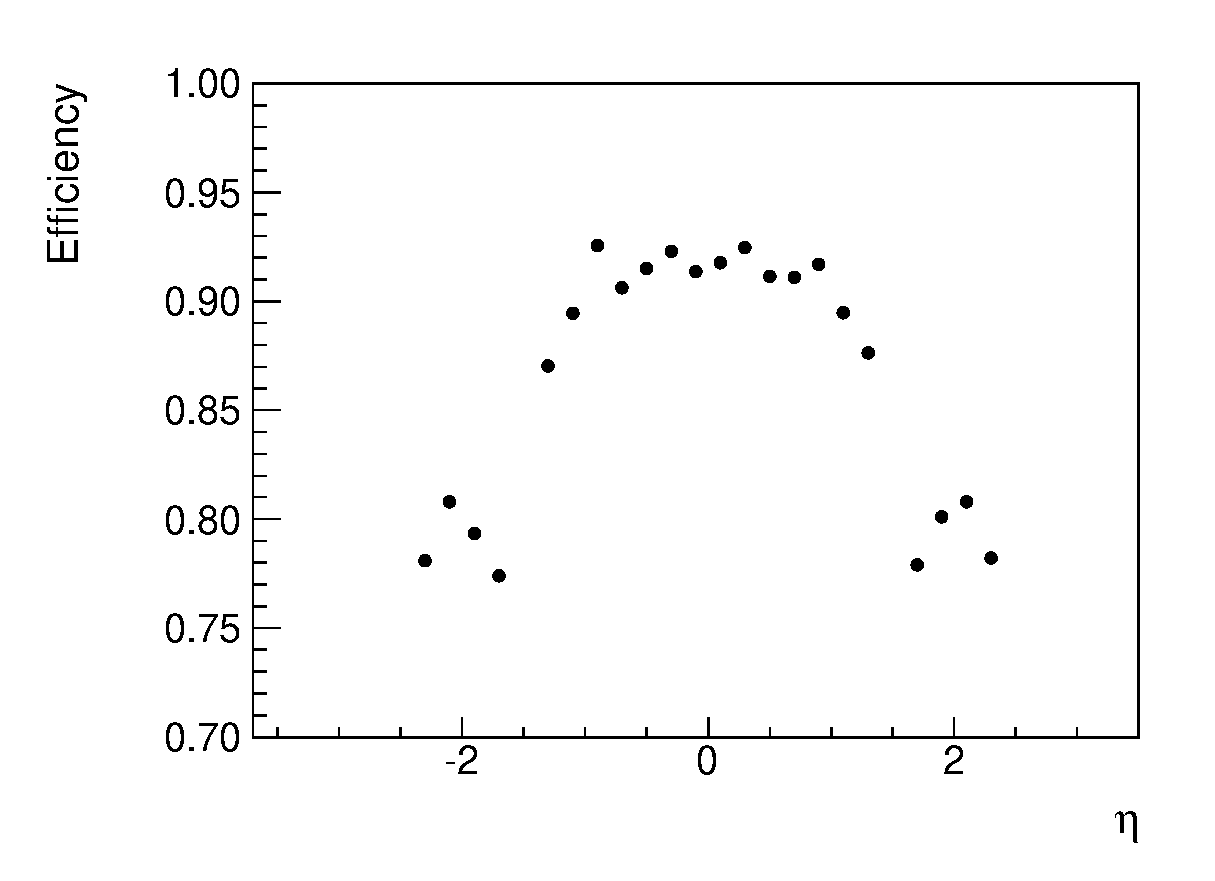
\includegraphics[width=0.49\textwidth]{plots/Efficiency_Total_Unbiased_Eta.eps} 
    \caption{A one dimensional projection of the electron selection efficiency computed from the Monte Carlo simulation, as a function of the $\eta$ of the electron.}
    \label{fig:FullElectronSelectionFromMC_Eta}
  \end{center}
\end{figure}

\begin{table}[ht]
  \begin{center}
    \large 
\footnotesize 
\begin{tabular}{|c|c|c|c|c|c|}\hline 
\backslashbox{$p_T [\GeVc]$}{$\eta$} & -2.50 To -2.00 & -2.00 To -1.50 & -1.50 To -1.00 & -1.00 To -0.50 & -0.50 To 0.00 \\ 
 \hline 
0.0  - 10.0 & 0.00 & 0.00 & 0.00 & 0.00 & 0.00 \\ 
10.0 - 20.0 & 0.75 & 0.59 & 0.81 & 0.82 & 0.86 \\ 
20.0 - 30.0 & 0.75 & 0.70 & 0.82 & 0.86 & 0.88 \\ 
30.0 - 40.0 & 0.80 & 0.79 & 0.89 & 0.92 & 0.92 \\ 
40.0 - 50.0 & 0.84 & 0.85 & 0.93 & 0.95 & 0.95 \\ 
50.0 - 60.0 & 0.84 & 0.87 & 0.94 & 0.95 & 0.95 \\ 
60.0 - 70.0 & 0.86 & 0.88 & 0.95 & 0.95 & 0.95 \\ 
70.0 - 80.0 & 0.83 & 0.89 & 0.95 & 0.96 & 0.97 \\ 
80.0 - 90.0 & 0.80 & 0.90 & 0.95 & 0.95 & 0.97 \\ 
 \hline 
\end{tabular} 
\begin{tabular}{|c|c|c|c|c|c|}\hline 
\backslashbox{$p_T [\GeVc]$}{$\eta$}  & 0.00 To 0.50 & 0.50 To 1.00 & 1.00 To 1.50 & 1.50 To 2.00 & 2.00 To 2.50 \\ 
 \hline 
0.0  - 10.0 & 0.00 & 0.00 & 0.00 & 0.00 & 0.00 \\ 
10.0 - 20.0 & 0.77 & 0.86 & 0.75 & 0.68 & 0.63 \\ 
20.0 - 30.0 & 0.88 & 0.86 & 0.83 & 0.71 & 0.76 \\ 
30.0 - 40.0 & 0.92 & 0.92 & 0.89 & 0.80 & 0.79 \\ 
40.0 - 50.0 & 0.95 & 0.95 & 0.93 & 0.85 & 0.84 \\ 
50.0 - 60.0 & 0.95 & 0.95 & 0.94 & 0.87 & 0.85 \\ 
60.0 - 70.0 & 0.95 & 0.96 & 0.94 & 0.88 & 0.85 \\ 
70.0 - 80.0 & 0.96 & 0.96 & 0.95 & 0.89 & 0.90 \\ 
80.0 - 90.0 & 0.96 & 0.95 & 0.96 & 0.90 & 0.92 \\ 
 \hline 
\end{tabular} 

  \end{center}
  \caption{\label{tab:FullElectronSelectionFromMC} The efficiency of the full electron selection criteria separated into bins of $p_{T}$ and $\eta$}.
\end{table}

In order to account for any differences in the behavior of the data and the Monte Carlo simulation, we measure efficiency scale factors corrections at various stages of the electron selection process. This is performed using the tag and probe methods introduced above. Correlations among the different efficiency scale factors are accounted for by imposing a particular order when computing the efficiencies, where the probes are required to satisfy all previous selection requirements. The efficiency scale factor is defined to be the ratio of the tag and probe efficiency measurement in data to the tag and probe efficiency measurement in the Monte Carlo simulation:

\begin{eqnarray}
  \label{eqn:EfficiencyScaleFactor}  
  S_{i}^{\mathrm{ele}} = \frac{\epsilon_{i}^{\mathrm{data}}}{\epsilon_{i}^{\mathrm{MC}}},
\end{eqnarray}

where $i$ label the various components of the full electron selection criteria described below.


Scale factors for the following components of the full electron selection criteria are derived:
\begin{itemize}
%\item $\epsilon_{\mathrm{supercluster}}^{\mathrm{ele}}$ : the efficiency of reconstructing a super cluster in the ECAL, given that an GSF track without the requirement of pixel seeding has been reconstructed,
\item $\epsilon_{\mathrm{gsftrk}}^{\mathrm{ele}}$ : the efficiency of reconstructing a GSF Track, given that a super cluster has been reconstructed in its direction,
\item $\epsilon_{\mathrm{gsfele}}^{\mathrm{ele}}$ : the efficiency of reconstructing a GSF Electron, given that a GSF Track has been matched in direction to a super cluster,
\item $\epsilon_{\mathrm{d0}}^{\mathrm{ele}}$ : the efficiency of the impact parameter cut, given that a GSF Electron has been reconstructed,
\item $\epsilon_{\mathrm{conv}}^{\mathrm{ele}}$ : the efficiency of the conversion veto, given that a GSF Electron has been reconstructed passing all above requirements,
\item $\epsilon_{\mathrm{iso}}^{\mathrm{ele}}$ : the efficiency of the isolation requirement, given that a GSF Electron has been reconstructed passing all above requirements,
\item $\epsilon_{\mathrm{id}}^{\mathrm{ele}}$ : the efficiency of the categorized identification criteria, given that a GSF Electron has been reconstructed passing all above requirements.
\end{itemize}

The total scale factor for the electron selection requirements is the product of the scale factors for each individual requirement:

\begin{eqnarray}
  \label{eqn:electronTotalEfficiencyScaleFactor}
  S^{\mathrm{ele}} = S_{\mathrm{gsftrk}}^{\mathrm{ele}} \times S_{\mathrm{gsfele}}^{\mathrm{ele}} \times  S_{\mathrm{d0}}^{\mathrm{ele}} \times  S_{\mathrm{conv}}^{\mathrm{ele}}  \times S_{\mathrm{iso}}^{\mathrm{ele}}  \times S_{\mathrm{id}}^{\mathrm{ele}}
\end{eqnarray}

This scale factor is measured in bins of $p_{T}$ and $\eta$. To obtain the final scale factor corrected electron selection efficiency, the efficiency measurement from the Monte Carlo simulation must be multiplied with this scale factor, bin by bin, and then convoluted with the $p_{T}$ and $\eta$ distribution of the Monte Carlo signal sample. 

We describe in detail the measurement for each of the above efficiencies using the tag and probe method as well as the results using the Monte Carlo simulation below. 

\customSubsubsection{GSF Track Reconstruction Efficiency}
To measure the efficiency that a GSF track is reconstructed, given that a super cluster has been reconstructed in the ECAL, we define probe electrons to be the reconstructed super clusters.  The GSF track reconstruction efficiency is then equal to the ratio of the number of probes for which there is a reconstructed GSF track within a cone of $\Delta$R $=\sqrt{\Delta\eta^{2}+\Delta\phi^{2}} = 0.1$, $N_{\mathrm{GSF-SC\ match}}$, to the number of super cluster probe ($N_{\mathrm{SC}}$):

\begin{eqnarray}
  \label{eqn:gsftrkEfficiency}  
  \epsilon_{\mathrm{gsftrk}}^{\mathrm{ele}} = \frac{N_{\mathrm{GSF-SC\ match}}}{\mathrm{N_{\mathrm{SC}}}},
\end{eqnarray}

The GSF track reconstruction efficiency measurements as a function of $p_{T}$ and $\eta$ using the tag and probe method are shown in Figure \ref{gsfTrackEfficiency_TagAndProbe}, where we compare the measurement using the zero background assumption and the measurement using a mass fit method described in detail in Section \ref{sec:MassFitMethod}. For the studies presented in this note, the Monte Carlo background has been added to the signal to produce a realistic representation of the data. The background involved in the measurement of the GSF track reconstruction efficiency is considerably larger compared to the background involved in the measurement of the other efficiency components. Thus, to control the systematic uncertainty due to the background estimation, we perform the measurement using a tighter mass range between $86\ \GeVcc$ and $96\ \GeVcc$.

\begin{figure}[htb]
  \begin{center}
    %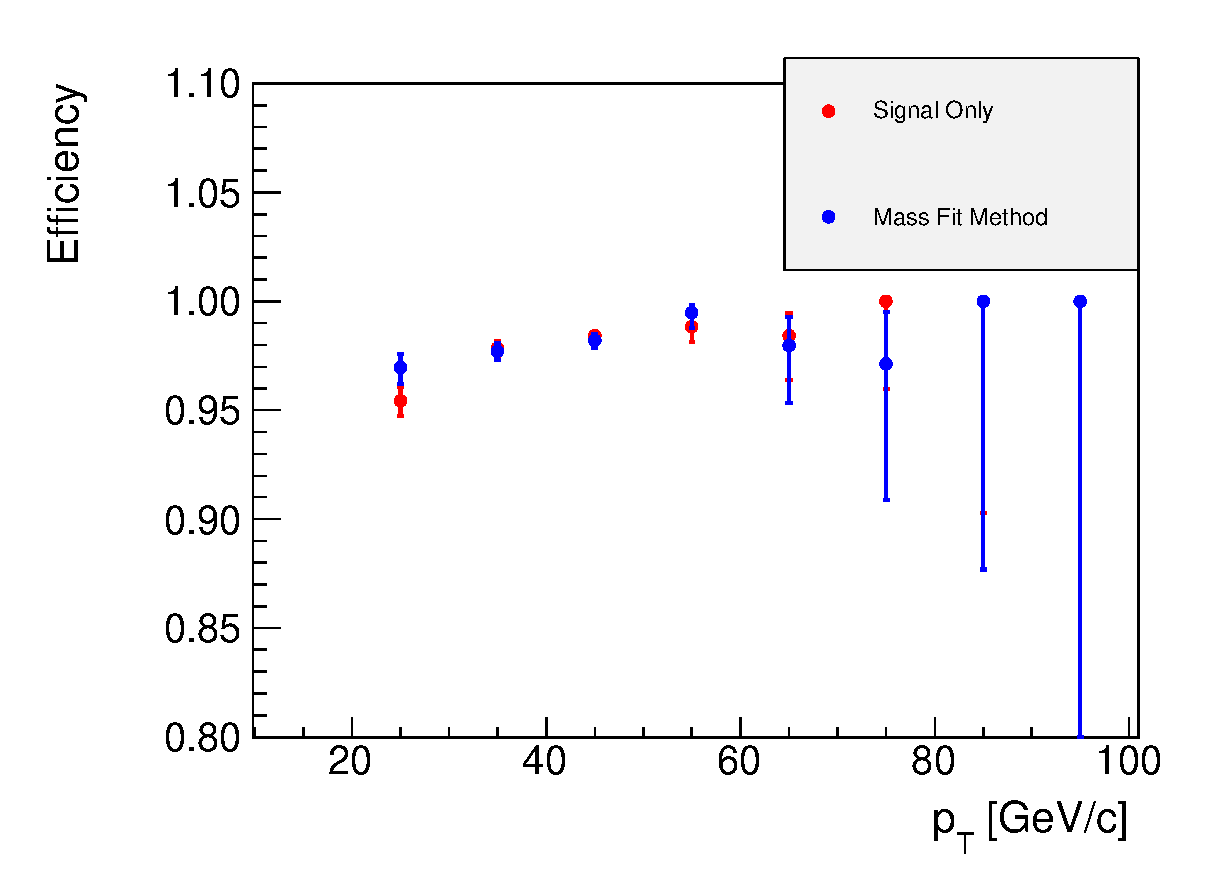
\includegraphics[width=0.49\textwidth]{plots/Efficiency_GsfTrack_Pt.eps} 
    \subfigure[]{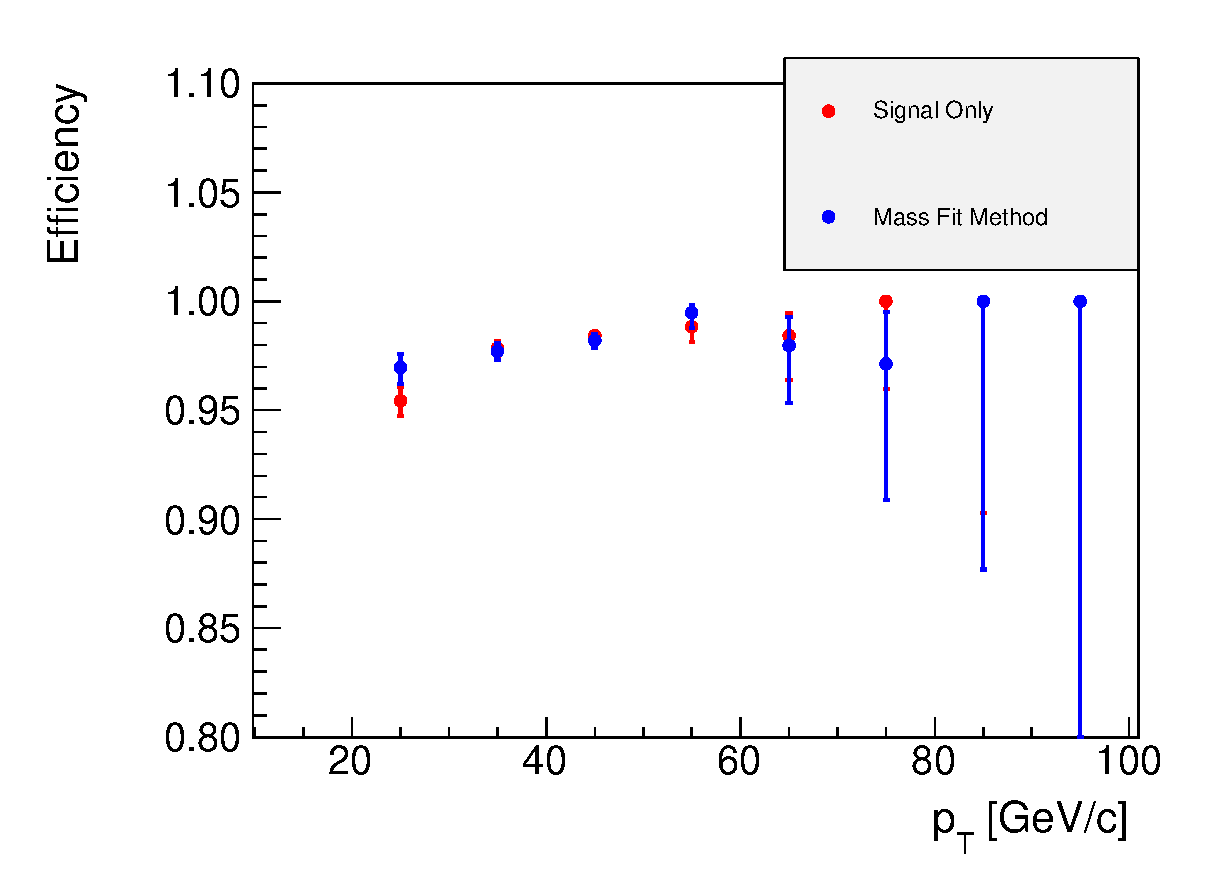
\includegraphics[width=0.49\textwidth]{plots/Efficiency_GsfTrack_Pt.eps}} 
    \subfigure[]{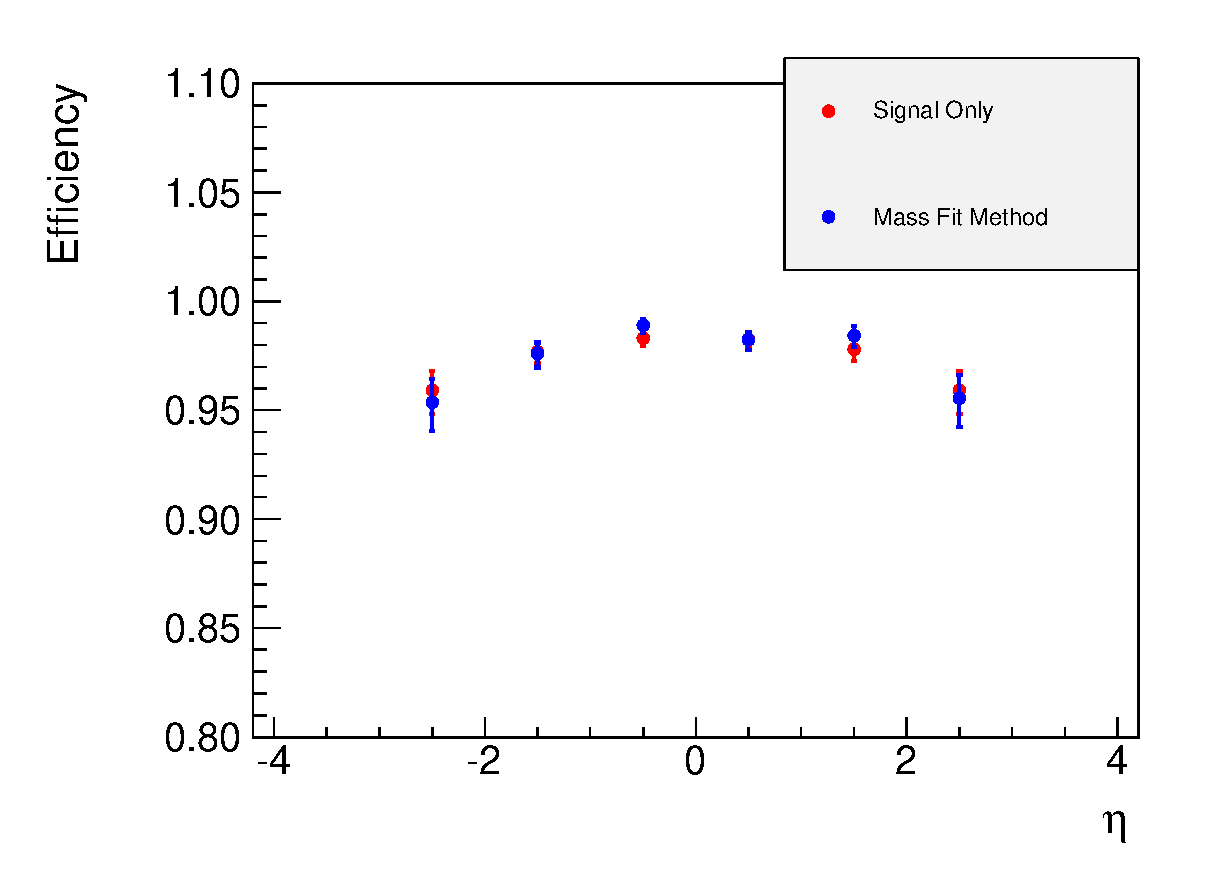
\includegraphics[width=0.49\textwidth]{plots/Efficiency_GsfTrack_Eta.eps}} 
    \caption{The efficiency for reconstructing a GSF track given that a super cluster was reconstructed in the same direction measured using the tag and probe method. The efficiency measurement from the signal Monte Carlo simulation is compared with the measurement using the mass fit background subtraction technique.}
    \label{gsfTrackEfficiency_TagAndProbe}
  \end{center}
\end{figure}


\customSubsubsection{GSF Electron Reconstruction Efficiency}
The efficiency for a GSF electron to be reconstructed is measured by defining a probe to be any GSF track that is matched to a super cluster to within $\Delta$R $< 0.1$. The efficiency is then equal to the number of such probes which have a reconstructed GSF electron candidate within $\Delta$R $< 0.1$, $N_{\mathrm{gsfele}}$, divided by the total number of such probes ($N_{\mathrm{GSF-SC\ match}}$):

\begin{eqnarray}
  \label{eqn:gsfeleEfficiency}  
  \epsilon_{\mathrm{gsfele}}^{\mathrm{ele}} = \frac{N_{\mathrm{gsfele}}}{(N_{\mathrm{GSF-SC\ match}})}
\end{eqnarray}

The GSF electron reconstruction efficiency measurements as a function of $p_{T}$ and $\eta$ using the tag and probe method are shown in Figure \ref{gsfElectronEfficiency_TagAndProbe}, where we compare the measurement using the zero background assumption and the measurement using the same-sign background estimation technique described in detail in Section \ref{sec:SameSignMethod}. The result shows that the same-sign background estimation technique adequately describes the true Monte Carlo simulation efficiency.

\begin{figure}[htb]
  \begin{center}
    \subfigure[]{\includegraphics[width=0.49\textwidth]{plots/Efficiency_GsfElectron_Pt.eps}} 
    \subfigure[]{\includegraphics[width=0.49\textwidth]{plots/Efficiency_GsfElectron_Eta.eps}} 
    \caption{The efficiency for reconstructing a GSF electron given a super cluster and GSF track matched in direction measured using the tag and probe method. The efficiency measurement from the signal Monte Carlo simulation is compared with the measurement using the same-sign background subtraction technique.}
    \label{gsfElectronEfficiency_TagAndProbe}
  \end{center}
\end{figure}




\customSubsubsection{Impact Parameter Cut Efficiency}
The efficiency for a GSF electron to pass the impact parameter cut is measured by defining a probe to be any GSF electron candidate. The efficiency is then equal to the number of such candidates passing the impact parameter cut ($N_{\mathrm{d0}}$) divided by the total number of such probes ($N_{\mathrm{gsfele}}$):

\begin{eqnarray}
  \label{eqn:electrond0cutEfficiency}  
  \epsilon_{d0}^{\mathrm{ele}} = \frac{N_{\mathrm{d0}}}{N_{\mathrm{gsfele}}}
\end{eqnarray}

In the absence of suitable collision data, we compare the impact parameter cut efficiency as a function of $p_{T}$ and $\eta$ obtained using the tag and probe method using the zero background assumption and using the same-sign background subtraction technique in Figure \ref{d0CutEfficiency_TagAndProbe}, showing that the same-sign background subtraction technique adequately describes the true Monte Carlo simulation efficiency.

\begin{figure}[htb]
  \begin{center}
    \subfigure[]{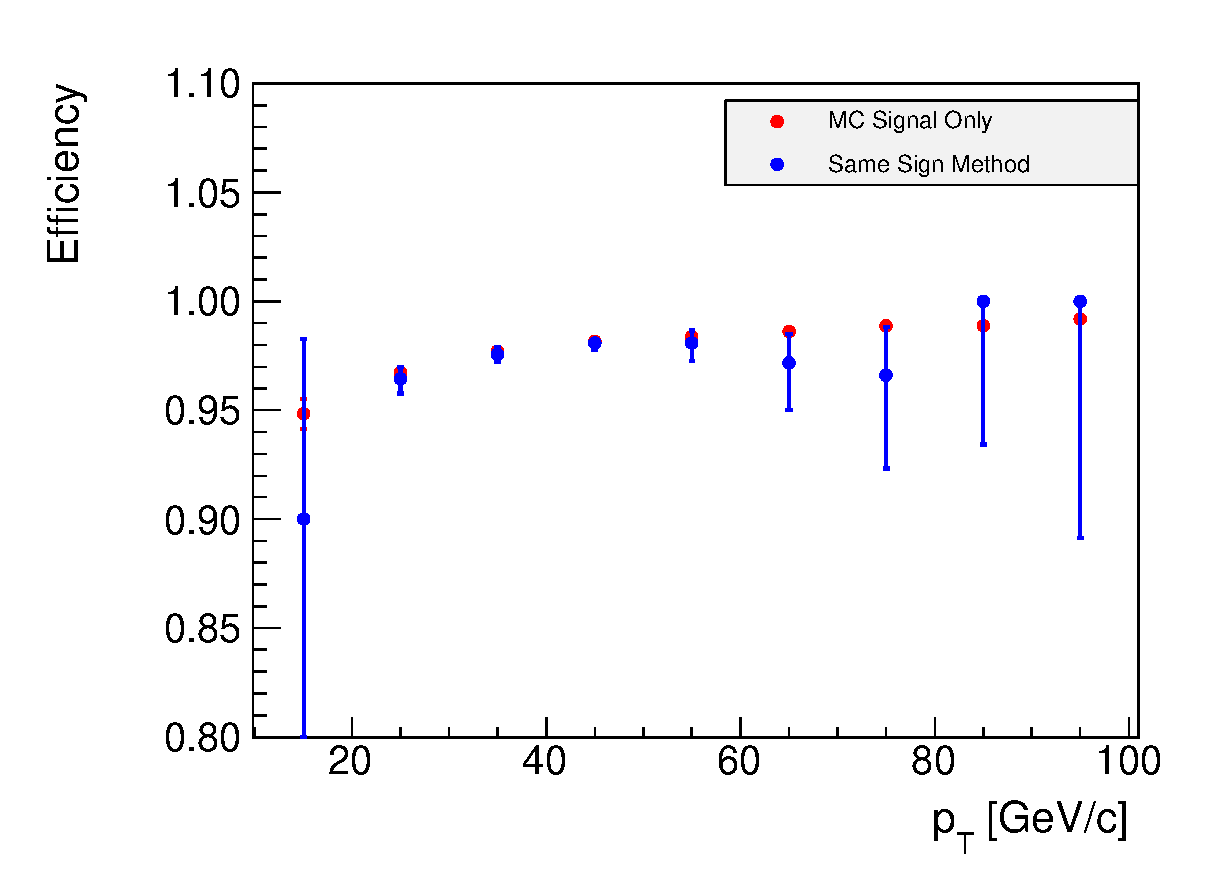
\includegraphics[width=0.49\textwidth]{plots/Efficiency_D0Cut_Pt.eps}} 
    \subfigure[]{\includegraphics[width=0.49\textwidth]{plots/Efficiency_D0Cut_Eta.eps}} 
    \caption{The electron impact parameter cut efficiency measured using the tag and probe method. The efficiency measurement from the signal Monte Carlo simulation is compared with the measurement using the same-sign background subtraction technique.}
    \label{d0CutEfficiency_TagAndProbe}
  \end{center}
\end{figure}


\customSubsubsection{Conversion Veto Efficiency}
The conversion veto efficiency is measured by defining a probe to be any GSF electron candidate which passes the impact parameter cut. The efficiency is then equal to the number of such candidates passing the conversion veto ($N_{\mathrm{conv}}$) divided by the total number of such probes ($N_{\mathrm{d0}}$):

\begin{eqnarray}
  \label{eqn:conversionVetoEfficiency}  
  \epsilon_{conv}^{\mathrm{ele}} = \frac{N_{\mathrm{conv}}}{N_{\mathrm{d0}}}
\end{eqnarray}

The conversion veto efficiency measurements as a function of $p_{T}$ and $\eta$ using the tag and probe method are shown in Figure \ref{convVetoEfficiency_TagAndProbe}, where we compare the measurement using the zero background assumption and the measurement using same-sign background estimation technique. The result shows that the same-sign background subtraction technique adequately describes the true Monte Carlo simulation efficiency.

\begin{figure}[htb]
  \begin{center}
    \subfigure[]{\includegraphics[width=0.49\textwidth]{plots/Efficiency_ConversionVeto_Pt.eps}} 
    \subfigure[]{\includegraphics[width=0.49\textwidth]{plots/Efficiency_ConversionVeto_Eta.eps}} 
    \caption{The conversion veto cut efficiency measured using the tag and probe method. The efficiency measurement from the signal Monte Carlo simulation is compared with the measurement using the same-sign background subtraction technique.}
    \label{convVetoEfficiency_TagAndProbe}
  \end{center}
\end{figure}


\customSubsubsection{Isolation Cut Efficiency}
The isolation cut efficiency is measured by defining a probe to be any GSF electron candidate which passes the impact parameter cut and the conversion veto. The efficiency is then equal to the number of such candidates passing the isolation cut ($N_{\mathrm{iso}}$) divided by the total number of such probes ($N_{\mathrm{conv}}$):

\begin{eqnarray}
  \label{eqn:electronIsolationEfficiency}  
  \epsilon_{iso}^{\mathrm{ele}} = \frac{N_{\mathrm{iso}}}{N_{\mathrm{conv}}}
\end{eqnarray}

The isolation cut efficiency measurements as a function of $p_{T}$ and $\eta$ using the tag and probe method are shown in Figure \ref{eleIsoCutEfficiency_TagAndProbe}, where we compare the measurement using the zero background assumption and the measurement using same-sign background estimation technique. The result shows that the same-sign background subtraction technique adequately describes the true Monte Carlo simulation efficiency. The apparently disagreement is due to systematic uncertainties resulting from the background subtraction. The plotted uncertainties do not include uncertainties in the subtracted background. These uncertainties are particularly large for these Monte Carlo backgrounds since they contain large weight events.  

\begin{figure}[htb]
  \begin{center}
    \subfigure[]{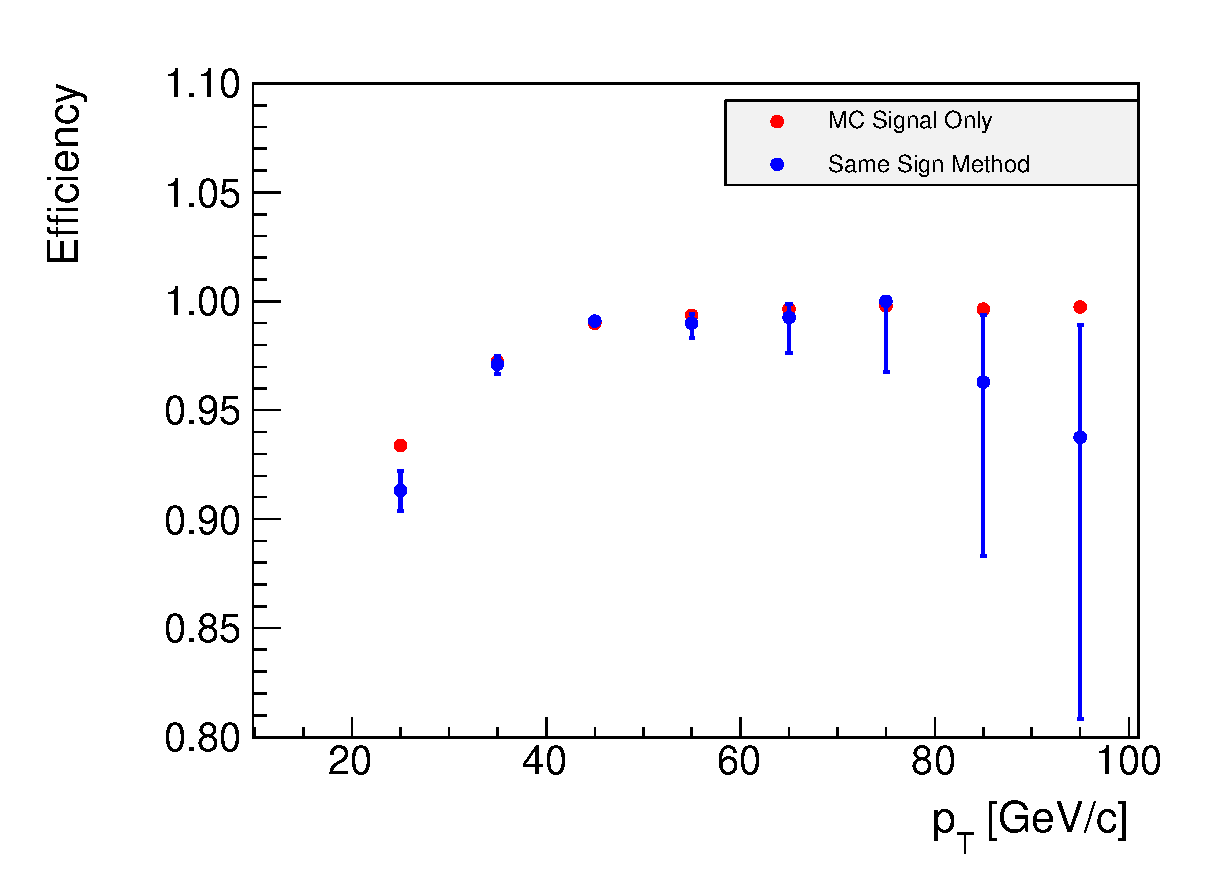
\includegraphics[width=0.49\textwidth]{plots/Efficiency_Isolation_Pt.eps}} 
    \subfigure[]{\includegraphics[width=0.49\textwidth]{plots/Efficiency_Isolation_Eta.eps}} 
    \caption{The isolation cut efficiency measured using the tag and probe method. The efficiency measurement from the signal Monte Carlo simulation is compared with the measurement using the same-sign background subtraction technique. }
    \label{eleIsoCutEfficiency_TagAndProbe}
  \end{center}
\end{figure}




\customSubsubsection{Electron ID Cut Efficiency}
The efficiency of the electron identification cuts is measured by defining a probe to be any GSF electron candidate which passes the impact parameter cut, the conversion veto, and the isolation cut. The efficiency is then equal to the number of such candidates passing the electron identification requirements ($N_{\mathrm{id}}$) divided by the total number of such probes ($N_{\mathrm{iso}}$):

\begin{eqnarray}
  \label{eqn:electronIDEfficiency}  
  \epsilon_{id}^{\mathrm{ele}} = \frac{N_{\mathrm{id}}}{N_{\mathrm{iso}}}
\end{eqnarray}

The measurements of the electron identification cuts as a function of $p_{T}$ and $\eta$ using the tag and probe method are shown in Figure \ref{eleIDCutEfficiency_TagAndProbe}, where we compare the measurement using the zero background assumption and the measurement using same-sign background estimation technique. The result shows that the same-sign background subtraction technique adequately describes the true Monte Carlo simulation efficiency.

\begin{figure}[htb]
  \begin{center}
    \subfigure[]{\includegraphics[width=0.49\textwidth]{plots/Efficiency_CustomTightID_Pt.eps}} 
    \subfigure[]{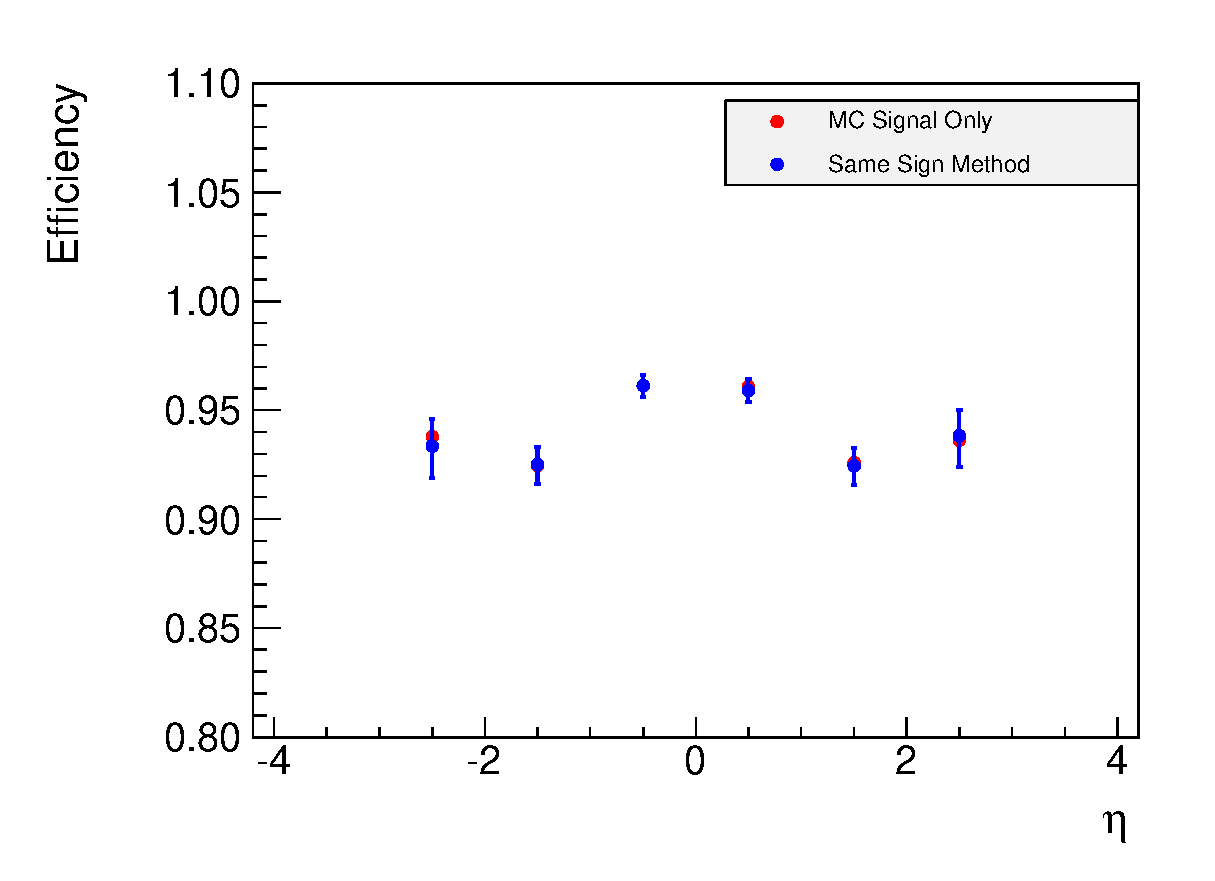
\includegraphics[width=0.49\textwidth]{plots/Efficiency_CustomTightID_Eta.eps}} 
    \caption{The electron identification cut efficiency measured using the tag and probe method. The efficiency measurement from the signal Monte Carlo simulation is compared with the measurement using the same-sign background subtraction technique.}
    \label{eleIDCutEfficiency_TagAndProbe}
  \end{center}
\end{figure}


\customSubsubsection{Total Electron Efficiency}
In the absence of suitable collision data, we present a summary of the efficiency measurements at all the various stages of electron selection neglecting the scale factor correction, in Table \ref{tab:electronEfficiencies} separated into the ECAL barrel (EB) and the ECAL end cap (EE) regions. The final efficiency for the electron selection is $90.7\%$ in the barrel, and $76.7\%$ in the endcap for the full sample of selected events. 

\begin{table}[!ht]
\begin{center}
\begin{tabular}{|c|c|c|c|}
\hline
 & \multicolumn{3}{|c|}{Electron Selection Efficiency} \\
\hline
 Selection Requirements & ECAL barrel (EB) & ECAL end cap (EE) & Total \\
\hline
\hline
 GSFTrack Reconstruction             & $99.1\%$  & $95.8\%$ & $98.1\%$ \\
 GSFElectron Reconstruction          & $99.2\%$  & $98.4\%$ & $99.0\%$ \\
 Impact Parameter Cut                & $99.2\%$  & $94.8\%$ & $97.9\%$ \\
 Conversion Veto Filter              & $99.4\%$  & $95.5\%$ & $98.2\%$ \\
 Electron Isolation Cut              & $97.7\%$  & $97.5\%$ & $97.6\%$ \\
 Electron ID Cuts                    & $95.6\%$  & $92.1\%$ & $94.6\%$ \\
\hline                               
 Total Electron Selection Efficiency & $90.7\%$  & $76.7\%$ & $86.2\%$ \\
\hline
\end{tabular}
\caption{The efficiency measurement for each individual electron selection cut, for all selected \Z\To\Ep\Em events assuming a scale factor of 1, and integrated over all $p_{T}$ and $\eta$ bins. \label{tab:electronEfficiencies}}
\end{center}
\end{table}

Due to the possibility of large variations in the performance of different detector systems, we separate the measurement into the three samples (EBEB, EBEE, EEEE) defined in Section \ref{sec:acceptance}. Since the distribution of kinematic quantities of electrons in these samples will be different from the distributions of kinematic quantities of electrons in the total sample, the efficiency measurement must be performed separately for these category of events. The analogous table of efficiencies are shown for the EBEB type events, the EBEE type events, and the EEEE type events in Tables \ref{tab:electronEfficiencies_EBEB}, \ref{tab:electronEfficiencies_EBEE}, and \ref{tab:electronEfficiencies_EEEE}, respectively. 


\begin{table}[!ht]
\begin{center}
\begin{tabular}{|c|c|}
\hline
 & Electron Selection Efficiency \\
\hline
 Selection Requirements & ECAL barrel (EB)  \\
\hline
\hline
 GSFTrack Reconstruction             & $99.2\%$   \\
 GSFElectron Reconstruction          & $99.3\%$   \\
 Impact Parameter Cut                & $99.3\%$   \\
 Conversion Veto Filter              & $99.4\%$   \\
 Electron Isolation Cut              & $97.9\%$   \\
 Electron ID Cuts                    & $95.7\%$   \\
\hline                               
 Total Electron Selection Efficiency & $91.0\%$   \\
\hline
\end{tabular}
\caption{The efficiency measurement for each individual electron selection cut, for selected \Z\To\Ep\Em events where both electrons are in the barrel region (EBEB) assuming a scale factor of 1. \label{tab:electronEfficiencies_EBEB}}
\end{center}
\end{table}

\begin{table}[!ht]
\begin{center}
\begin{tabular}{|c|c|c|c|}
\hline
 & \multicolumn{3}{|c|}{Electron Selection Efficiency} \\
\hline
 Selection Requirements & ECAL barrel (EB) & ECAL end cap (EE) & Total \\
\hline
\hline
 GSFTrack Reconstruction             & $99.1\%$  & $96.2\%$ & $97.6\%$ \\
 GSFElectron Reconstruction          & $99.1\%$  & $98.1\%$ & $98.6\%$ \\
 Impact Parameter Cut                & $99.2\%$  & $94.6\%$ & $96.9\%$ \\
 Conversion Veto Filter              & $99.4\%$  & $95.8\%$ & $97.6\%$ \\
 Electron Isolation Cut              & $97.1\%$  & $97.1\%$ & $97.1\%$ \\
 Electron ID Cuts                    & $95.7\%$  & $91.3\%$ & $93.6\%$ \\
\hline                               
 Total Electron Selection Efficiency & $89.9\%$  & $76.8\%$ & $82.7\%$ \\
\hline
\end{tabular}
\caption{The efficiency measurement for each individual electron selection cut, for selected \Z\To\Ep\Em events where one electron is in the barrel region and one electron is in the endcap region (EBEE) assuming a scale factor of 1. \label{tab:electronEfficiencies_EBEE}}
\end{center}
\end{table}

\begin{table}[!ht]
\begin{center}
\begin{tabular}{|c|c|}
\hline
 & Electron Selection Efficiency \\
\hline
 Selection Requirements &  ECAL end cap (EE) \\
\hline
\hline
 GSFTrack Reconstruction             & $96.5\%$  \\
 GSFElectron Reconstruction          & $98.7\%$  \\
 Impact Parameter Cut                & $94.9\%$  \\
 Conversion Veto Filter              & $94.8\%$  \\
 Electron Isolation Cut              & $98.3\%$  \\
 Electron ID Cuts                    & $93.4\%$  \\
\hline                               
 Total Electron Selection Efficiency & $78.8\%$  \\
\hline
\end{tabular}
\caption{The efficiency measurement for each individual electron selection cut, for selected \Z\To\Ep\Em events where both electrons are in the endcap region (EEEE) assuming a scale factor of 1. \label{tab:electronEfficiencies_EEEE}}
\end{center}
\end{table}


\customSubsection{Electron Trigger Efficiency}
The efficiency for an event to fire the single electron L1 and HLT trigger path given that it has passed all offline selection criteria must be measured in order to measure the total event selection efficiency. The primary method used to measure this efficiency is the tag and probe method relying on well reconstructed $\Z$ boson events that are selected from the single lepton triggers. First, two leptons passing the full lepton selection criteria are required, whose invariant mass is between $70\ \GeVcc$ and $110\ \GeVcc$. In order to eliminate bias due to the leading lepton trigger object, one has to veto the leading lepton trigger object from the efficiency measurement. The other lepton is used as a probe to determine the efficiency that a lepton passing the full lepton selection criteria will fire the trigger. However doing this yields an incorrect determination of the trigger efficiency due to combinatorics, when the leading lepton trigger object and the second lepton being used as a probe fall within the same $p_T$ and $\eta$ bin. This problem can be overcome, for those cases, by randomly selecting one of the two leptons and requiring that one of the two fires the trigger. The remaining object is used as the probe. The single electron trigger efficiency measured in Monte Carlo simulation is shown as a function of its transverse momentum and the pseudorapidity in Figure \ref{fig:SingleElectronTriggerEfficiency_TagAndProbeMethod}, where the statistical uncertainties shown are those achievable with $10\ \ipb$ of collision data. An efficiency scale factor will be similarly derived for the trigger efficiency measurements by comparing the data measurement with the measurement from the Monte Carlo simulation.

\begin{figure}[htb]
  \begin{center}
    \subfigure[]{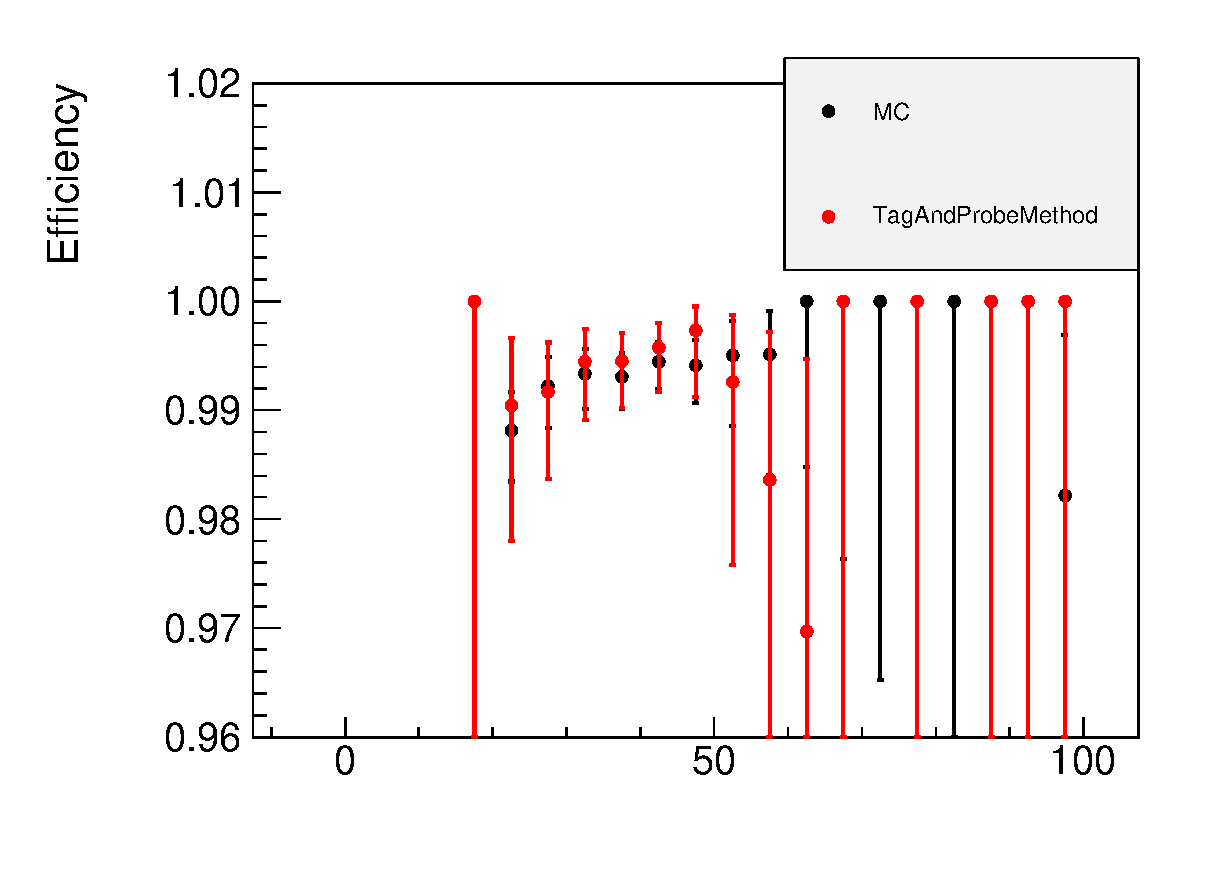
\includegraphics[width=0.49\textwidth]{plots/Efficiency_ElectronTrigger_TagAndProbeMethod_Pt.eps}} 
    \subfigure[]{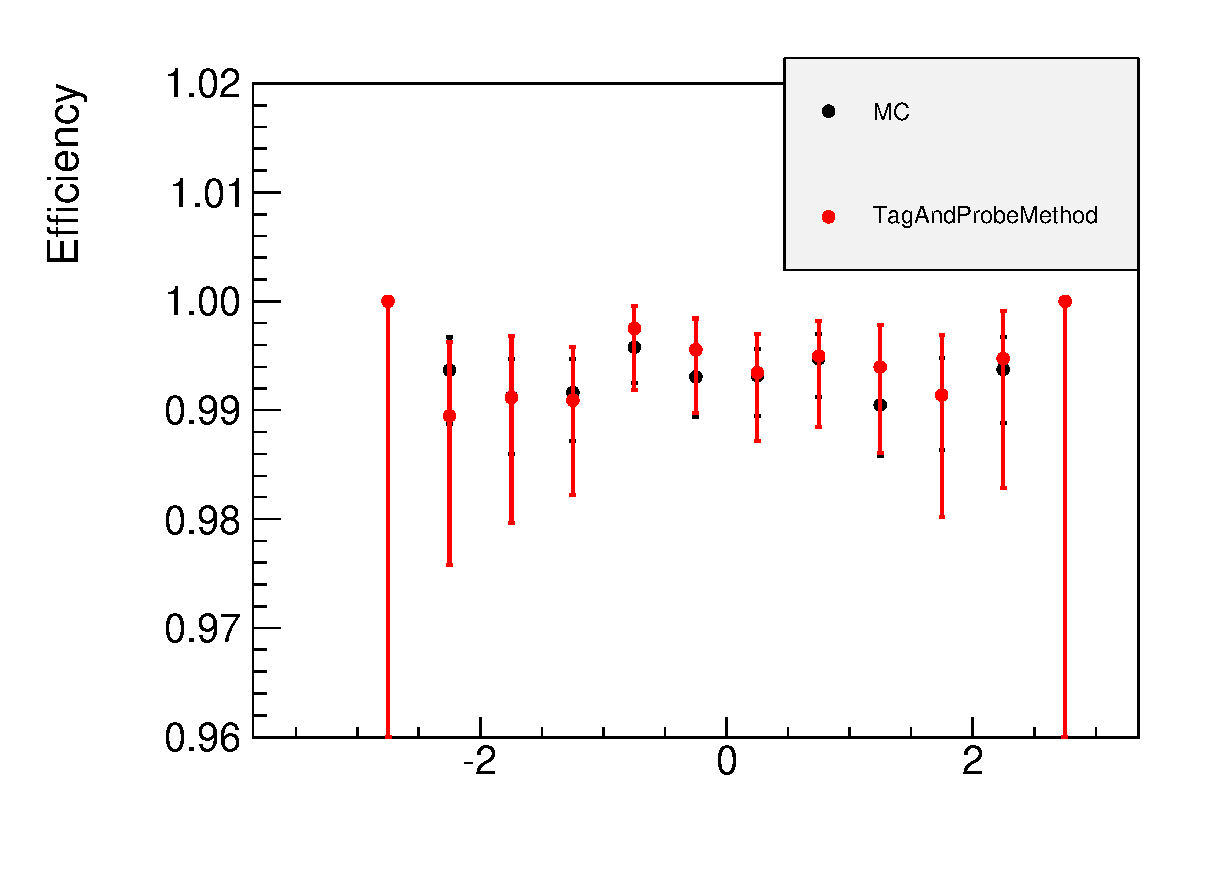
\includegraphics[width=0.49\textwidth]{plots/Efficiency_ElectronTrigger_TagAndProbeMethod_Eta.eps}} 
    \caption{The single electron trigger efficiency measured in Monte Carlo simulation as a function of the $p_{T}$ and $\eta$ of the object. }
    \label{fig:SingleElectronTriggerEfficiency_TagAndProbeMethod}
  \end{center}
\end{figure}


An alternative cross check of the single lepton trigger efficiency measurement can be made using events collected by orthogonal triggers. We use events that fire the Jet30 trigger and select any leptons that passes the full lepton selection criteria and does not lie within $\Delta$R $< 0.3$ cone of the leading trigger jet as a probe for the single lepton trigger efficiency. Figure \ref{fig:SingleElectronTriggerEfficiency_TagAndProbeMethod} shows the measurement of the single electron trigger efficiency as a function of the transverse momentum and pseudorapidity in Monte Carlo simulation with uncertainties representing the statistical uncertainty achievable with $10\ \ipb$ of data.

\begin{figure}[htb]
  \begin{center}
    \subfigure[]{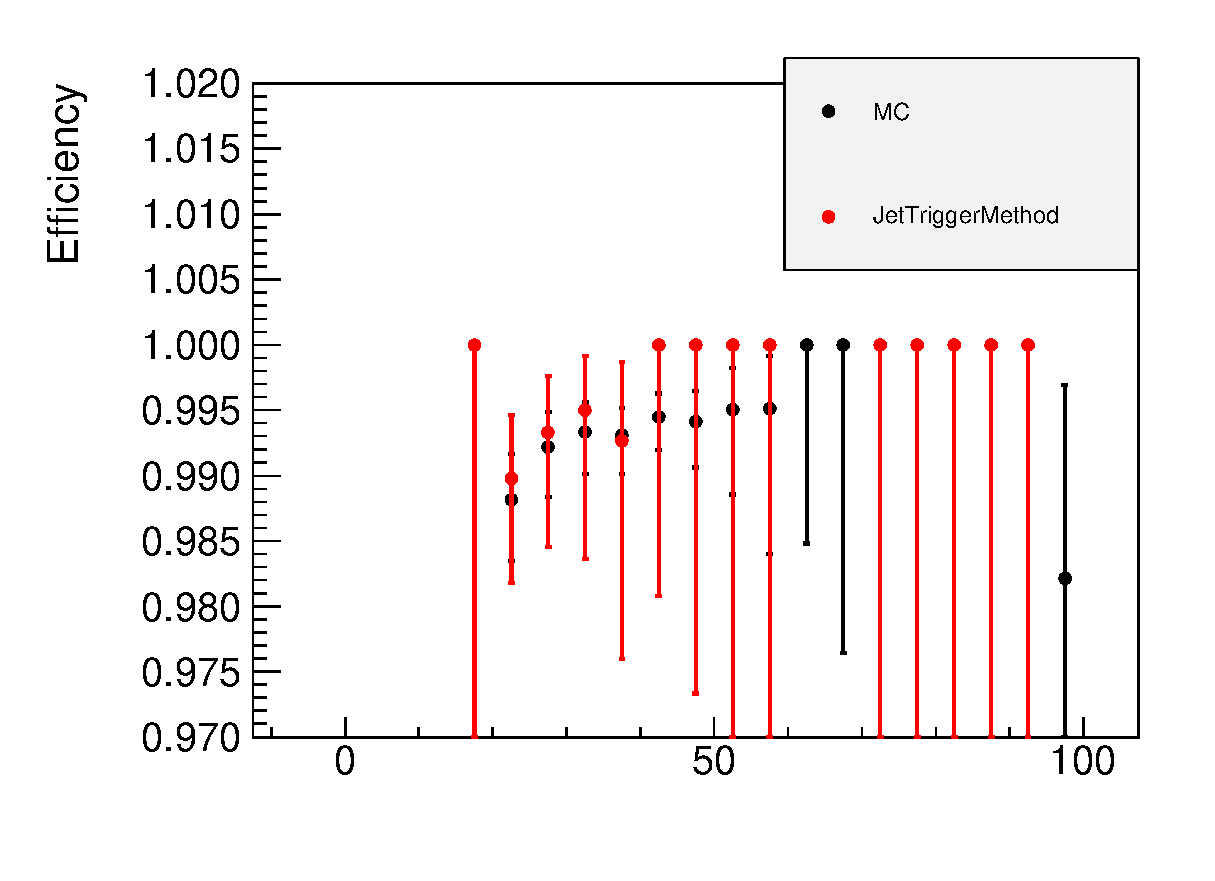
\includegraphics[width=0.49\textwidth]{plots/Efficiency_ElectronTrigger_JetTriggerMethod_Pt.eps}} 
    \subfigure[]{\includegraphics[width=0.49\textwidth]{plots/Efficiency_ElectronTrigger_JetTriggerMethod_Eta.eps}} 
    \caption{The single electron trigger efficiency measured in Monte Carlo simulation as a function of the $p_{T}$ and $\eta$ of the object. }
    \label{fig:SingleElectronTriggerEfficiency_JetTriggerMethod}
  \end{center}
\end{figure}


\customSubsection{Background Subtraction in Efficiency Measurements}
\label{sec:TagAndProbeBackground}
Since background events have much lower efficiency to pass the electron selection criteria than signal events, one has to properly account for background contributions in order to obtain an accurate signal efficiency measurement. We describe a number of techniques that are used to account for background contributions. Since the backgrounds contributing to the efficiency measurement are identical to the backgrounds for the \Z\To\Ep\Em event selection, the methods used are fully described in Section \ref{sec:Backgrounds}. 

\customSubsubsection{Same-Sign Method}
\label{sec:SameSignMethodForEfficiency}
For denominator probes which have a determined charge, it is possible to use the event yield for the same-sign sample as an estimate of the background for the opposite-sign sample, after properly accounting for signal contributions to the same-sign sample. This method is described in more detail in Section \ref{sec:SameSignMethod}.  To show the performance of this background subtraction method, a comparison of the transverse momentum distribution of the probe electrons for the isolation cut efficiency measurement between the opposite-sign and same-sign sample in Monte Carlo simulation is shown in Figure \ref{fig:probept_bkgSSOS}. Figure \ref{fig:probept_signalMCVsSSMethod} shows a comparison of the signal Monte Carlo and the prediction for the signal using the same-sign background subtraction method.

%The main background contributions are from QCD multijet and $\gamma+$jet events for which the electric charges of the two leptons are uncorrelated. As a result, one can use a data sample consisting of two leptons with the same electric charge to predict the total background contribution. The same-sign sample is dominated by background, but for the dielectron final state there is a contribution from signal \Z\To\Ep\Em events where one of the electrons undergoes hard bremstrahlung and then subsequently converts. These contributions are accounted for by using the Monte Carlo simulation prediction. After this correction is made, the total background contribution is equal to two times the event yield for the same-sign sample. This technique can be used in all cases where an electric charge can be associated with the probe electron. A comparison of the transverse momentum distribution of the probe electrons for the isolation cut efficiency measurement between the opposite-sign and same-sign sample in Monte Carlo simulation is shown in Figure \ref{fig:probept_bkgSSOS}. Figure \ref{fig:probept_signalMCVsSSMethod} shows a comparison of the signal Monte Carlo and the prediction for the signal using the background subtraction method described above.

\begin{figure}[htb]
  \begin{center}
    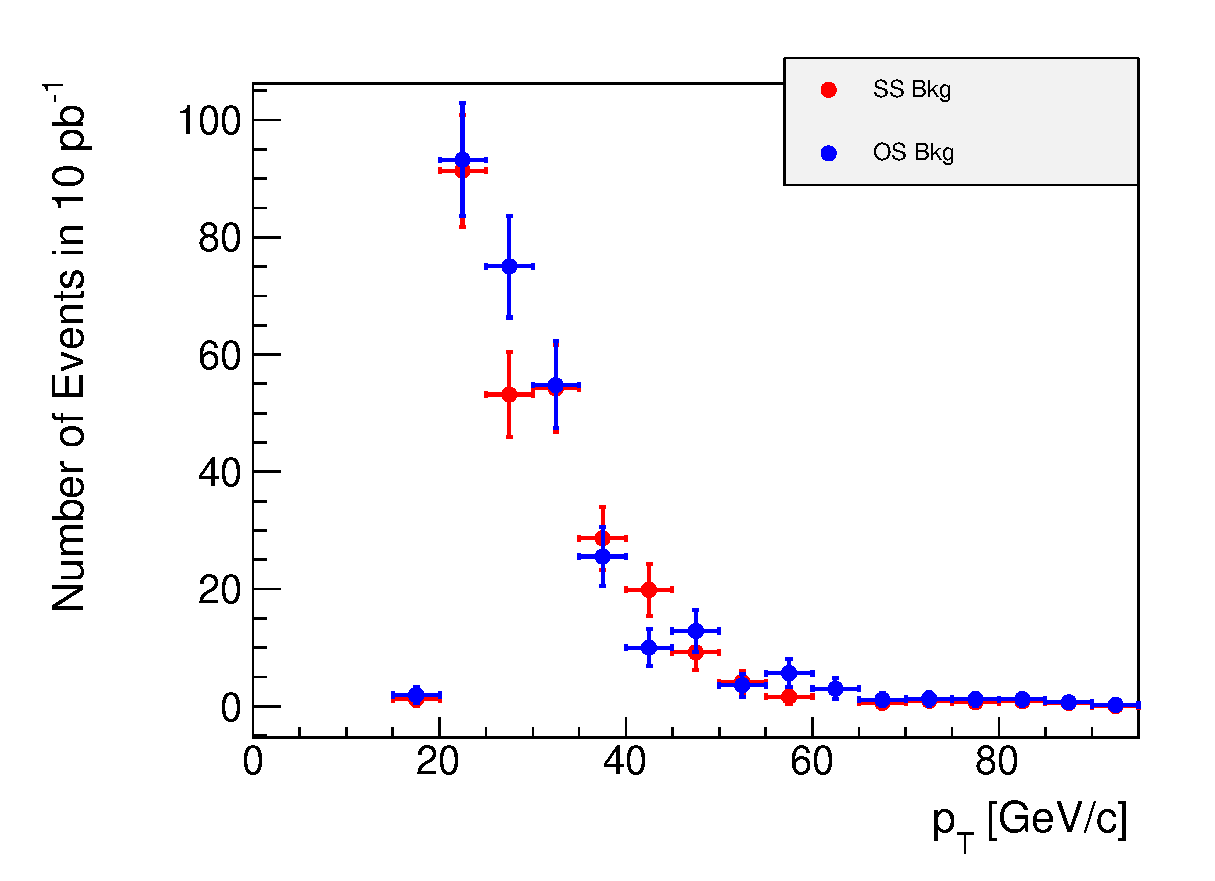
\includegraphics[width=0.6\textwidth]{plots/Efficiency_Isolation_Denominator_Pt_BkgSSOSComparison.eps}
    \caption{The probe electron transverse momentum distribution for the same-sign and opposite-sign background samples. }
    \label{fig:probept_bkgSSOS}
  \end{center}
\end{figure}

\begin{figure}[htb]
  \begin{center}
    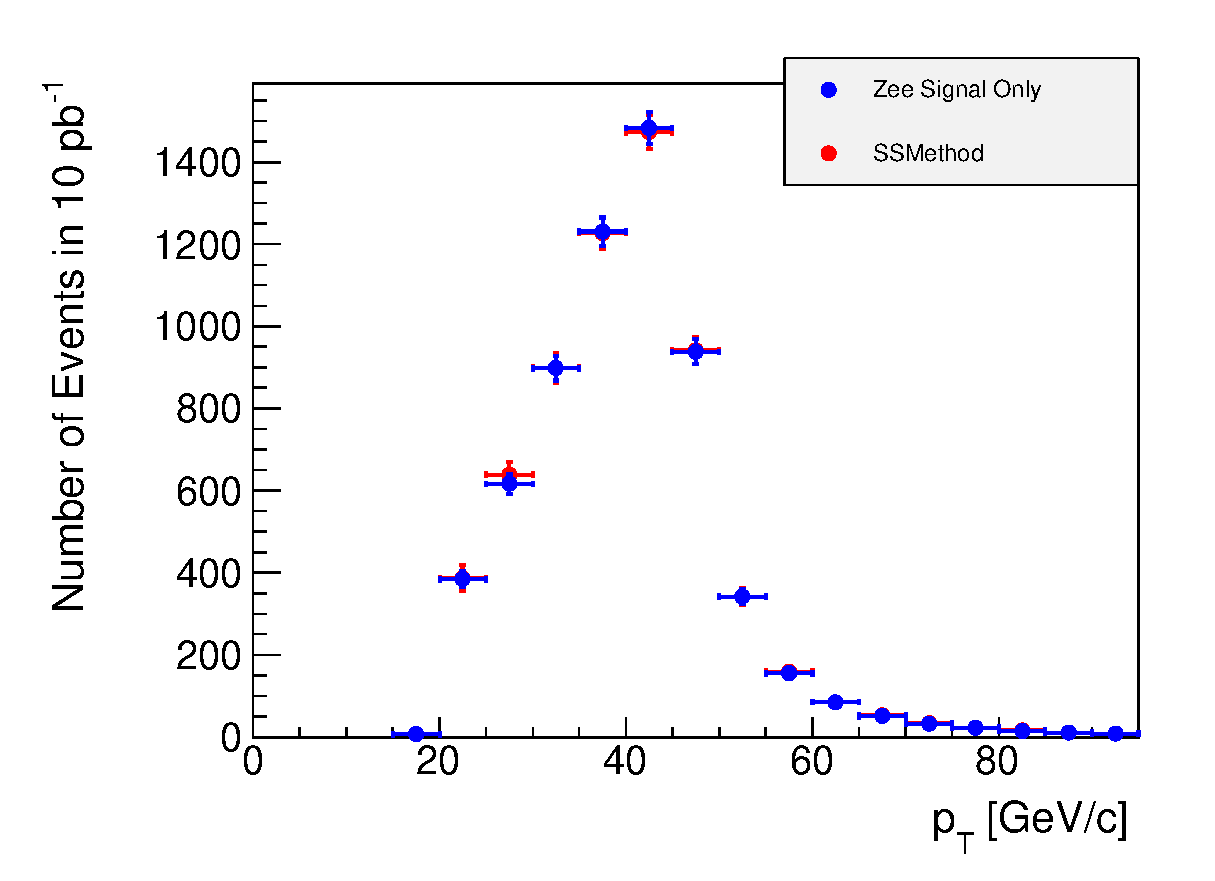
\includegraphics[width=0.6\textwidth]{plots/Efficiency_Isolation_Denominator_Pt_SSMethod.eps}
    \caption{The probe electron transverse momentum distribution for the signal Monte Carlo sample and the background subtracted signal prediction using the same-sign method. }
    \label{fig:probept_signalMCVsSSMethod}
  \end{center}
\end{figure}


%There is a non-neglible background contribution from the W$+$jets process, where one of the two leptons originates from a jet. There are significant correlations between the charge of the \W and the charge of a quark if the jet originates from a quark. In these cases, since a jet that mimics the signature of a lepton must be isolated and therefore typically must fragment to a leading charged particle, this charge correlation is largely preserved through the fragmentation and hadronization process. As a result, there are significant charge correlations for this component of the background. The charge correlation for these types of events as predicted by the Monte Carlo simulation are shown in Figure \ref{fig:WenuChargeCorrelation_TagAndProbe}. Comparing the contribution of the \W$+$jet background to the contribution of the QCD multijet and $\gamma+$jet background, shown in Figure \ref{TagAndProbeGsfElectronBackgrounds_Lepton2Pt} for a reconstructed GSF electron in the Tag and Probe selection, one concludes that the contribution from the \W$+$jet background is small and therefore this effect has only a minor impact on the final efficiency measurement.
%% \begin{figure}[htb]
%%   \begin{center}
%%     \includegraphics[width=0.49\textwidth]{plots/TagAndProbeGsfElectronBackgrounds_Lepton2Pt.eps} 
%%     \caption{The transverse momentum distribution of the second electron in the tag and probe selection, separated into the different background processes.}
%%     \label{fig:TagAndProbeGsfElectronBackgrounds_Lepton2Pt}
%%   \end{center}
%% \end{figure}



\customSubsubsection{Dilepton Mass Fit}
\label{sec:MassFitMethod}
An alternative approach is to make use of the well known line shape of the $\Z$ boson to fit the dilepton mass distribution with some model for the background. A reasonably simple background model that can be used is a linear background model. The function representing the Drell-Yan mass shape is given in Equation \ref{eqn:DrellYanMassFormula}, and includes propagator terms for the photon and the $\Z$ Boson and the term describing the interference between them. 

\begin{eqnarray}
  \label{eqn:DrellYanMassFormula} 
\frac{d\sigma_{\mathrm{signal}}}{dm} = N \left(\frac{\Gamma_{\mathrm{Z}}^{2} m^{2}/M_{\mathrm{Z}}^4}{(m^{2} - M_{\mathrm{Z}}^{2})^{2} + m^{4} \Gamma_{\mathrm{Z}}^{2} m^{2}/M_{\mathrm{Z}}^4} + \beta\frac{m^{2} - M_{\mathrm{Z}}^{2}}{(m^{2} - M_{\mathrm{Z}}^{2})^{2} + m^{4}\Gamma{\mathrm{Z}}^{2}/M_{\mathrm{Z}}^{2}} + \gamma\frac{1}{m^{2}} \right)
\end{eqnarray}

The Drell-Yan mass shape function is then convoluted with a modified gaussian resolution function, given in Equation \ref{eqn:ZMassResolutionFormula}, which takes into account the low side tail from final state radiation and bremstrahlung. 

\begin{eqnarray}
  \label{eqn:ZMassResolutionFormula} 
f(m) = \int \frac{d\sigma_{\mathrm{signal}}}{dm'}(m')G(m-m';\sigma,\alpha) dm' \\
G(x;\sigma,\alpha) = 
\begin{cases}
  e^{\frac{-x^{2}}{2\sigma^{2}+\alpha x^{2}}}  & x < 0 \\
  e^{\frac{-x^{2}}{2\sigma^{2}}}  & x >= 0
\end{cases}
\end{eqnarray}

An example of the fit of the signal from Monte Carlo is shown in Figure \ref{fig:ZeeMassFit_SignalOnly}, where the statistical uncertainties have been scaled to correspond to the statistical uncertainty in a $10$ $\ipb$ sample. 

\begin{figure}[htb]
  \begin{center}    
    \subfigure[]{\includegraphics[width=0.49\textwidth]{plots/Efficiency_GsfElectronDenominator_Mass_MCSignal.eps}} 
    \subfigure[]{\includegraphics[width=0.49\textwidth]{plots/Efficiency_GsfElectronDenominator_Mass_MCSignal_logY.eps}} 

    \caption{The dielectron mass distribution for tag and probe pairs defined for the GSF electron reconstruction efficiency measurement, shown along with the fitted model of the signal. No background is included in this plot. }
    \label{fig:ZeeMassFit_SignalOnly}
  \end{center}
\end{figure}

The linear background model is shown in Equation \ref{eqn:LinearBkgFormula}, where $N_{\mathrm{bkg}}$ is the factor required for normalization in the range that is considered by the fit. The final dielectron mass shape parameterization is shown in Equation \ref{eqn:SignalPlusBkgFormula}. The model parameters that enter the fit are summarized in Table \ref{tab:ZeeFitParameters}. 


%% OLD background parameterization
%% \begin{eqnarray}
%%   \label{eqn:LinearBkgFormula} 
%% \frac{d\sigma_{\mathrm{bkg}}}{dm} = N_{\mathrm{bkg}}(1 + \delta m)
%% \end{eqnarray}


%%NEW
\begin{eqnarray}
  \label{eqn:LinearBkgFormula} 
\frac{d\sigma_{\mathrm{bkg}}}{dm} = N_{\mathrm{bkg}}(\epsilon + \delta (m - m_{2} )
\end{eqnarray}

\begin{eqnarray}
  \label{eqn:ExponentialBkgFormula} 
\frac{d\sigma_{\mathrm{bkg}}}{dm} = N_{\mathrm{bkg}}(\epsilon + \delta e^{\chi m}(m - m_{2}))
\end{eqnarray}
%% NEW


\begin{eqnarray}
  \label{eqn:SignalPlusBkgFormula} 
\frac{d\sigma_{\mathrm{total}}}{dm} = N\left((1-f_{\mathrm{bkg}})\frac{d\sigma_{\mathrm{signal}}}{dm} + f_{\mathrm{bkg}} \frac{d\sigma_{\mathrm{bkg}}}{dm} \right)
\end{eqnarray}


\begin{table}[!ht]
\begin{center}
\begin{tabular}{|c|c|c|}
\hline
 Parameter & Description & Comment \\
\hline
N                          & Overall normalization                 & \\
$M_{\mathrm{Z}}$           & Mass of the \Z Boson                  & fixed to $91.2$ in the fit\\
$\Gamma_{\mathrm{Z}}$      & Width of the \Z Boson                 & fixed to $2.5$ in the fit\\
$\beta$                    & Coefficient of the interference term  & \\
$\gamma$                   & Coefficient of the photon term        & \\
$\sigma$                   & Gaussian mass resolution parameter    & \\
$\alpha$                   & Low mass tail factor                  & \\
$\delta$                   & Slope of the linear background        & \\
$f_{\mathrm{bkg}}$         & Background fraction                   & \\
\hline                               
\end{tabular}
\caption{Short description of the model parameters that enter the dielectron mass fit. \label{tab:ZeeFitParameters}}
\end{center}
\end{table}


The results of the fit is only used to extract the background estimate, which must be subtracted from the numerator and denominator in order to compute the signal efficiency. An example of the signal and background fit is shown in Figure \ref{fig:ZeeMassFit_SignalPlusBkg}. 

\begin{figure}[htb]
  \begin{center}
    \subfigure[]{\includegraphics[width=0.49\textwidth]{plots/Efficiency_GsfElectronNumerator_Mass_Data.eps}} 
    \subfigure[]{\includegraphics[width=0.49\textwidth]{plots/Efficiency_GsfElectronDenominator_Mass_Data_logY.eps}} 
    \caption{The dielectron mass distribution for tag and probe pairs defined for the GSF electron reconstruction efficiency measurement, shown along with the fitted model shown in the black curve and the background component of the model shown in the red line. Signal and background contributions are included. }
    \label{fig:ZeeMassFit_SignalPlusBkg}
  \end{center}
\end{figure}

The uncertainties on the two fit parameters relevent to the background can be used to estimate systematic uncertainties on the efficiency measurement by computing the difference in the efficiency estimate when the parameters are independantly varied up and down. This is further discussed in Section \ref{efficiencySystematicUncertainties}.

One refinement of this method is to simultaneously fit the events partitioned into the same sign and opposite sign samples. One additional parameter, the ratio of the same sign to opposite sign signal yield, is added to the model, shown in Equation \ref{eqn:SSOSSignalPlusBkgFormula}.  An example of the simultaneous fit is shown in Figure \ref{fig:ZeeSSOSMergedMassFit_SignalPlusBkg}. The systematic uncertainties are significantly reduced, since the simultaneous fit gives greater constraint on the background model.

\begin{eqnarray}
  \label{eqn:SSOSSignalPlusBkgFormula} 
\frac{d\sigma^{a}_{\mathrm{total}}}{dm} =  
\begin{cases}
  N\left( (1-f_{bkg})\frac{d\sigma_{\mathrm{signal}}}{dm} + f_{bkg} \frac{d\sigma_{\mathrm{bkg}}}{dm} \right), & a = \mathrm{OS} \\
    N\left( (1-f_{bkg})R_{\mathrm{SSOS}}\frac{d\sigma_{\mathrm{signal}}}{dm} + f_{bkg} \frac{d\sigma_{\mathrm{bkg}}}{dm} \right), & a = \mathrm{SS} \\
\end{cases}
\end{eqnarray}

\begin{figure}[htb]
  \begin{center}
    \subfigure[]{\includegraphics[width=0.49\textwidth]{plots/Efficiency_GsfElectron_Denominator_Mass_OS.eps}} 
    \subfigure[]{\includegraphics[width=0.49\textwidth]{plots/Efficiency_GsfElectron_Denominator_Mass_SS.eps}} 
    \caption{The dielectron mass distributions for tag and probe pairs defined for the GSF electron reconstruction efficiency measurement, shown separately for the opposite sign (a) and same sign (b) samples, along with the fitted model shown in the black curve and the background component of the model shown in the red line. }
    \label{fig:ZeeSSOSMergedMassFit_SignalPlusBkg}
  \end{center}
\end{figure}




\customSubsection{Efficiency Measurement Summary}
Finally, using the efficiency measurements presented in Section \ref{sec:electronEfficiency}, one can obtain the total event selection efficiency as defined in Equation \ref{eqn:totalEfficiency}. The efficiencies for the \Z\To\Ep\Em selection are summarized in Table \ref{tab:finalZeeEventSelectionEfficiency}, separately for the EBEB, EBEE, and EEEE events. 


\begin{table}[!ht]
\begin{center}
\begin{tabular}{|c|c|c|c|}
\hline
 & \multicolumn{3}{|c|}{Electron Selection Efficiency} \\
\hline
 Sample & $\epsilon_{\mathrm{offline}}$ & $\epsilon_{\mathrm{online}}$ & Total Efficiency \\
\hline
\hline
 EBEB                    & $0.910 \times 0.910$  &  $1.0$ & $0.828$ \\
 EBEE                    & $0.899 \times 0.768$  &  $1.0$ & $0.690$ \\
 EEEE                    & $0.788 \times 0.788$  &  $1.0$ & $0.621$ \\
 Full sample             & $0.862 \times 0.862$  &  $1.0$ & $0.743$ \\
\hline                               
\end{tabular}
\caption{The final \Z\To\Ep\Em event selection efficiency.  \label{tab:finalZeeEventSelectionEfficiency}}
\end{center}
\end{table}



\customSection{Backgrounds}
\label{sec:Backgrounds}
There are physics processes that can mimic the \Z\To\Ep\Em signature. They broadly fall under two different categories. The first category are electroweak processes where two real, prompt, and isolated electrons are produced. These backgrounds are estimated using the Monte Carlo simulation, which are expected to yield reasonably accurate predictions. The accuracy of the Monte Carlo prediction will be verified in the analysis of other control samples enhanced in each of the respective background processes. The second category involves processes where one or both of the electrons originate from photons or jets and are misidentified as an electron. The Monte Carlo simulation is not expected to model this background particularly well due to large theoretical uncertainties in the fragmentation model and in the detector material model employed in the simulation. As a result, this background is best predicted using data-driven techniques. 

After all event selection cuts, it is found that the total background contributes roughly $0.4\%$ of the total event yield. Thus the background contribution is of minor importance to the cross section measurement. Nonetheless, we describe in detail the methods used to obtain the estimate of the background.

\customSubsection{Electroweak Background}

The real lepton background is estimated using the Monte Carlo simulation. The events include $\Z$ decays to two tau leptons which subsequently decay to two electrons, production of a top and anti-top quark pair where both quarks decay to leptonic final states, and electroweak production of two vector bosons both decaying leptonically. The estimated event yield of these backgrounds for $10\ \ipb$ after the \Z\To\Ep\Em event selection requirements are shown in Table \ref{tab:zeeEwkBkg}. 

\begin{table}[!ht]
\begin{center}
\begin{tabular}{|c|c|}
\hline
\multicolumn{2}{|c|}{Events with both electrons in the ECAL Barrel (EBEB)} \\
\hline
 Process & Event Yield for $10\ \ipb$ \\
\hline
 $\Z \To \Taup\Taum$        & $0.5 \pm 0.7$  \\
 \ttbar                     & $2.3 \pm 1.5$  \\
 WW                         & $0.4 \pm 0.6$  \\
 WZ                         & $1.7 \pm 1.3$  \\
 ZZ                         & $1.0 \pm 1.0$  \\
\hline
\hline

\multicolumn{2}{|c|}{Events with one electron in the ECAL Barrel and one in the ECAL Endcap (EBEE)} \\
\hline
 Process & Event Yield for $10\ \ipb$ \\
\hline
 $\Z \To \Taup\Taum$        & $0.3 \pm 0.5$  \\
 \ttbar                     & $0.8 \pm 0.9$  \\
 WW                         & $0.3 \pm 0.6$  \\
 WZ                         & $0.6 \pm 0.8$  \\
 ZZ                         & $0.5 \pm 0.7$  \\
\hline
\hline

\multicolumn{2}{|c|}{Events with both electrons in the ECAL Endcap (EEEE)} \\
\hline
 Process & Event Yield for $10\ \ipb$ \\
\hline
 $\Z \To \Taup\Taum$        & $0.1  \pm 0.3$  \\
 \ttbar                     & $0.1  \pm 0.3$  \\
 WW                         & $0.02 \pm 0.1$  \\
 WZ                         & $0.3  \pm 0.6$  \\
 ZZ                         & $0.2  \pm 0.4$  \\
\hline

\end{tabular}
\caption{The electroweak background event yield for $10\ \ipb$ after all \Z\To\Ep\Em event selection cuts. These backgrounds are estimated from Monte Carlo simulation. \label{tab:zeeEwkBkg}}
\end{center}
\end{table}


\customSubsection{Fake Lepton Backgrounds}
The background processes involving fake leptons include W+Jet production where one electron originates from the decay of the W boson and the other is a jet misdentified as an electron, and QCD multijet events where both electrons are jets misidentified as leptons. There are also contributions from the W+$\gamma$ process, where the second lepton is a photon which converts asymmetrically such that one leg of the conversion carries almost all the momentum of the photon, and from the $\gamma$+jet process where one lepton is a photon that faked an electron and the other is a jet misidentified as an electron. 

\customSubsubsection{Same-Sign Method}
\label{sec:SameSignMethod}
Since the majority of these backgrounds yield reconstructed electrons whose charges are uncorrelated, it is possible to use the sample of events where both electrons are measured to have the same electric charge to predict the total background. It is possible for the \Z\To\Ep\Em signal event to enter the same-sign sample if one of the electrons undergoes hard bremstrahlung and subsequently converts in the asymmetric fashion. These contributions must be predicted using the Monte Carlo simulation and subtracted from the same-sign data sample. Since the charge of the leptons for these fake lepton backgrounds are uncorrelated, one expects that the number of same charge events is equal to the number of opposite charge events. Thus the total background is simply twice the number of events in the same-sign data sample, after subtracting the signal contribution. 

In the W+Jet process, there is a significant correlation between the charge of the lepton from the decay of the W boson and the charge of an outgoing quark. Since a jet that mimics the signature of a lepton must be isolated and therefore typically must fragment to a leading charged particle, this charge correlation is largely preserved through the fragmentation and hadronization process. As a result, there are significant charge correlations between the real lepton and the fake lepton for this component of the background. This can be seen in Figure \ref{fig:WenuChargeCorrelation_TagAndProbe} which shows the charge correlation between the two electron candidates in the $\W+$jets Monte Carlo simulation sample. For the purpose of most of the efficiency measurements, the contribution of the \W$+$jet background is small compared to the contribution of the QCD multijet and $\gamma+$jet background. This is illustrated in Figure \ref{fig:TagAndProbeElectronEfficiency_Isolation_Numerator_Stack_mcBkg_Pt}, showing the relative contribution of all backgrounds to the transverse momentum distribution of the numerator for the isolation efficiency measurement. Therefore this effect has only a minor impact on the efficiency measurements. Any remaining difference must be accounted for as a systematic uncertainty for the efficiency measurements and the background estimate.

\begin{figure}[htb]
  \begin{center}
    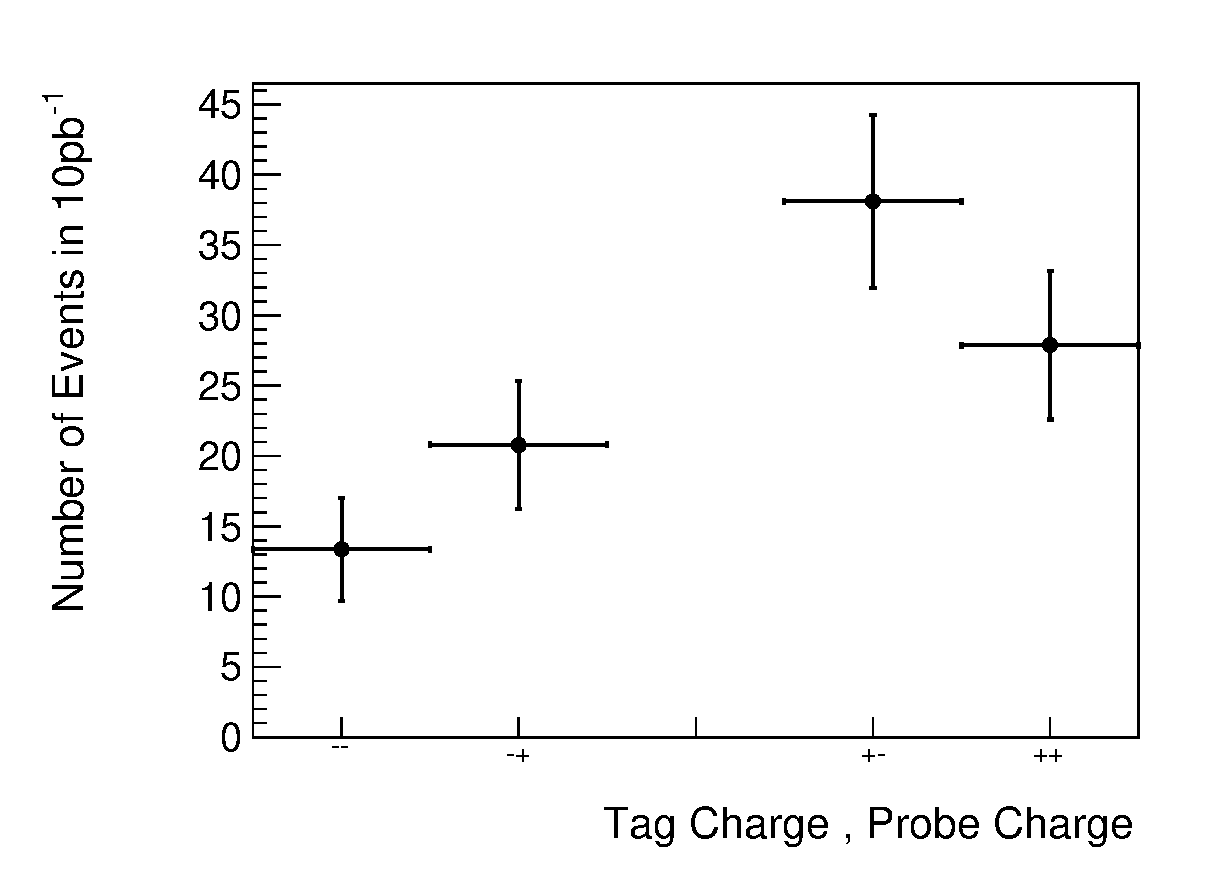
\includegraphics[width=0.6\textwidth]{plots/WenuChargeCorrelation_TagAndProbe.eps} 
    \caption{The distribution of the charge of the tag electron and the probe electron for \W\To\E\Nu$+$jets events. The first charge in the bin label indicates the charge of the tag electron, while the second charge indicates the charge of the probe electron. }
    \label{fig:WenuChargeCorrelation_TagAndProbe}
  \end{center}
\end{figure}

\begin{figure}[htb]
  \begin{center}
    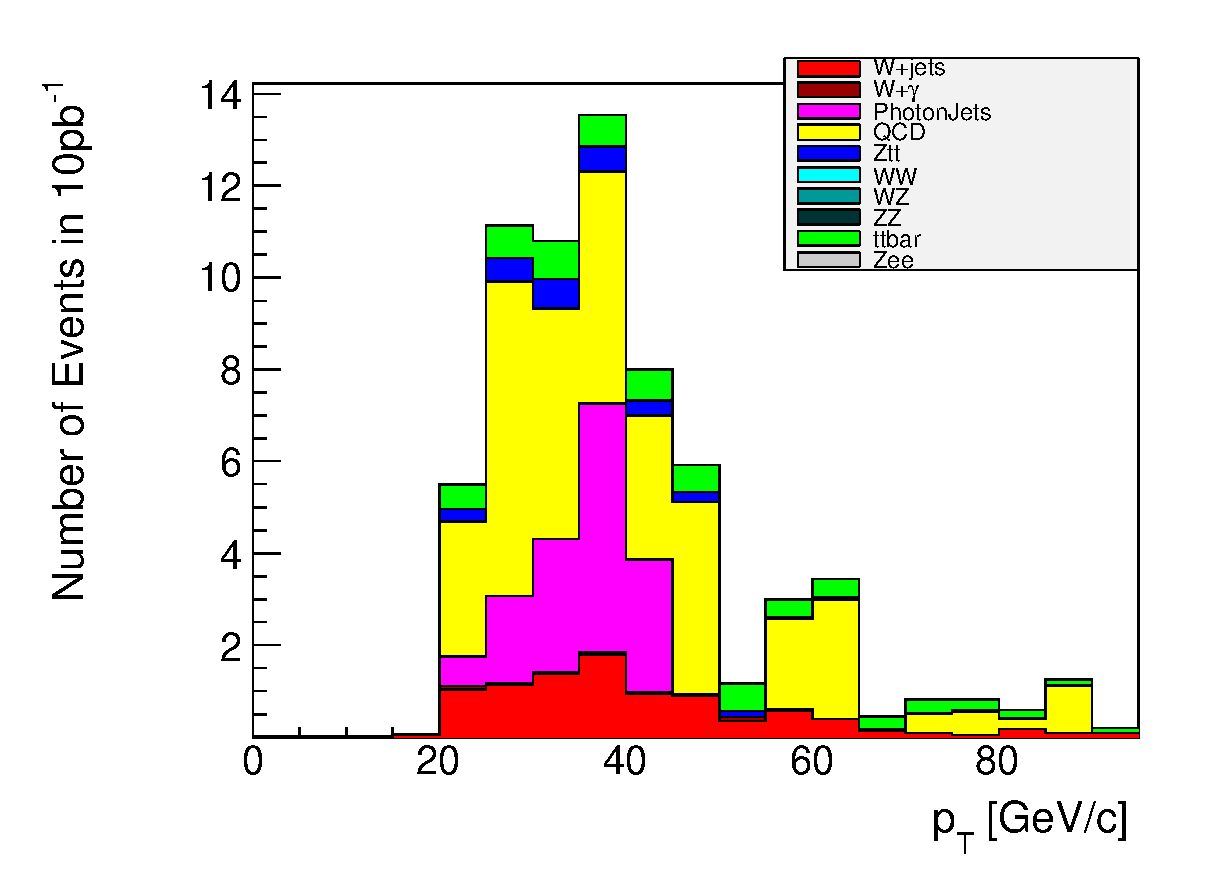
\includegraphics[width=0.6\textwidth]{plots/Efficiency_Isolation_Numerator_Stack_mcBkg_Pt.eps} 
    % From macro: ComputeTagAndProbeElectronEfficiency_MakeDetailedPlots.C
    \caption{The transverse momentum distribution of the numerator for the electron isolation efficiency measurement, where contributions from the various background processes have been shown separately. }
    \label{fig:TagAndProbeElectronEfficiency_Isolation_Numerator_Stack_mcBkg_Pt}
  \end{center}
\end{figure}

The dilepton mass distribution for the same-sign sample and the opposite-sign sample are shown in Figure \ref{zeeDileptonMass_HadBkg_Stack}, separating the contributions from the different hadronic background processes. A comparison of the hadronic background event yield prediction for the \Z\To\Ep\Em event selection obtained from the Monte Carlo simulation and that obtained using the same-sign method is shown in Figure \ref{zeeDileptonMass_HadBkg_MCVsSSMethod}. The two predictions agree to within statistical uncertainties and the difference is primarily due to having a lack of simulated events.

\begin{figure}[htb]
  \begin{center}
    \subfigure[]{\includegraphics[width=0.49\textwidth]{plots/zeeDileptonMass_HadBkg_SS_Stack.eps}} 
    \subfigure[]{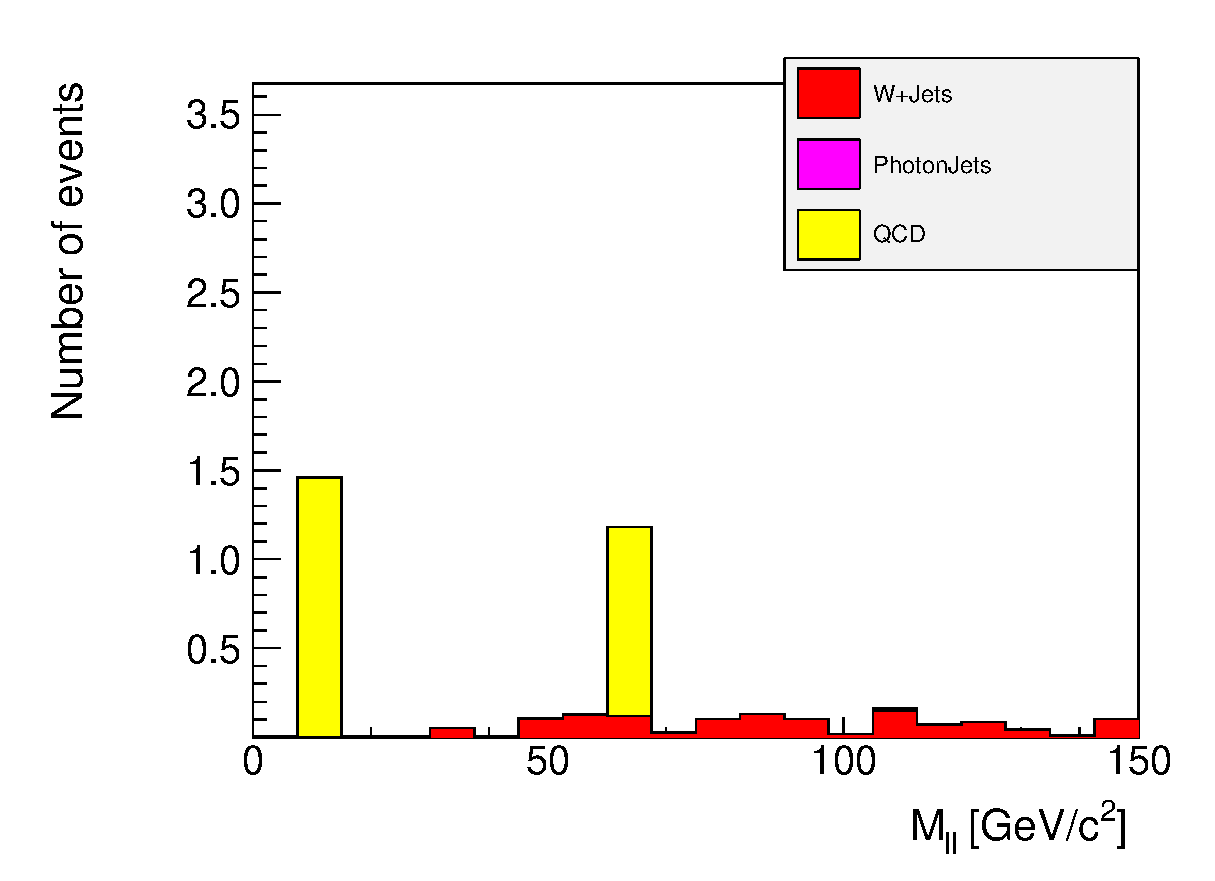
\includegraphics[width=0.49\textwidth]{plots/zeeDileptonMass_HadBkg_OS_Stack.eps}} 
    % from macro : ~/Tools/root/ZeeAnalysis/ZeeSameSignMethodPlots.C
    \caption{The Monte Carlo simulation dilepton mass distribution prediction for the hadronic background after the \Z\To\Ep\Em event selection for events where both leptons have the same sign (a) and events where the two leptons have opposite signs (b) for $10\ \ipb$ of data. Contributions from the different hadronic background processes are shown separately and stacked on top of each other.}
    \label{zeeDileptonMass_HadBkg_Stack}
  \end{center}
\end{figure}


\begin{figure}[htb]
  \begin{center}
    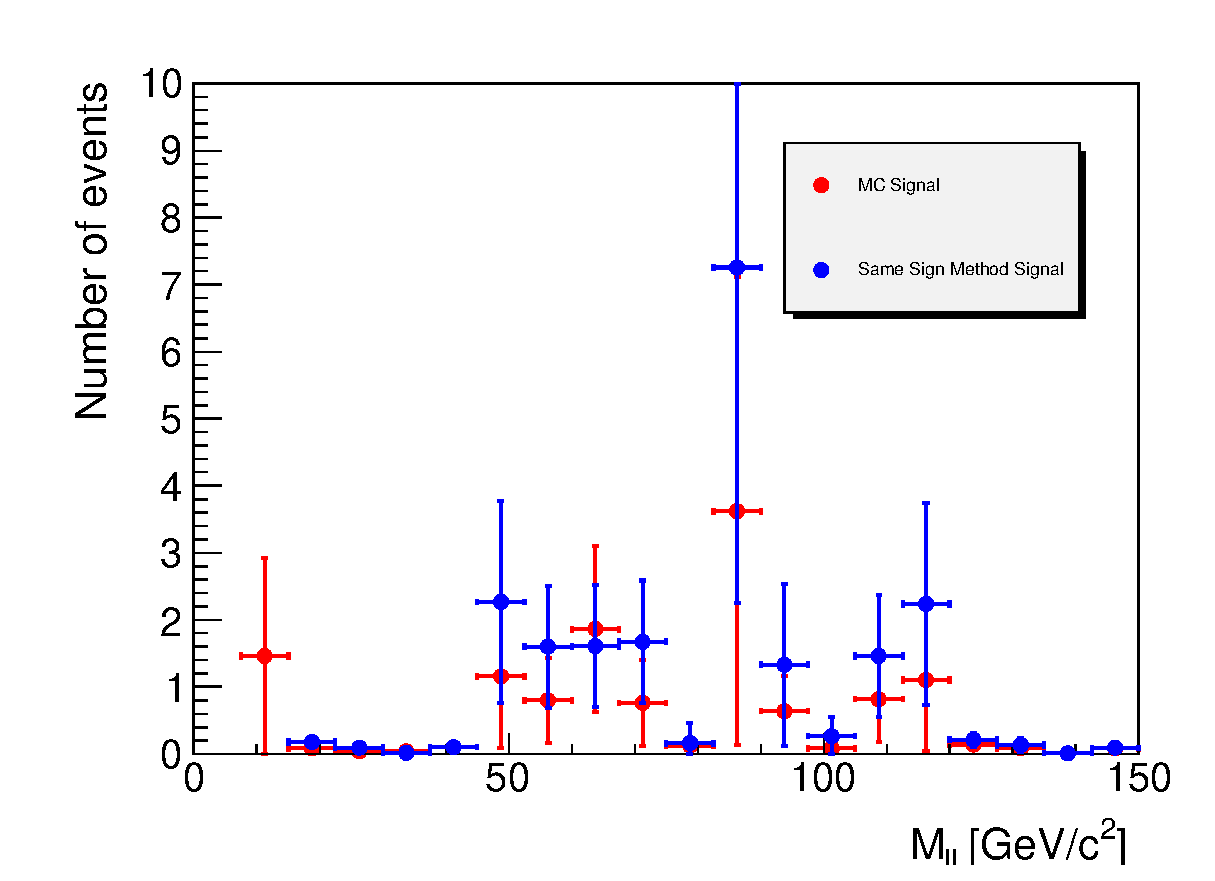
\includegraphics[width=0.49\textwidth]{plots/zeeDileptonMass_HadBkg_MCVsSSMethod.eps} 
    \caption{A comparison of the dilepton mass distribution prediction for the hadronic backgrounds for the \Z\To\Ep\Em event selection obtained from the Monte Carlo simulation and from the same-sign method. }
    \label{zeeDileptonMass_HadBkg_MCVsSSMethod}
  \end{center}
\end{figure}



\begin{table}[!ht]
\begin{center}
\begin{tabular}{|c|c|c|}
\hline
 Process & Same-Sign Method Event Yield for $10\ \ipb$ & Monte Carlo Simulation Event Yield for $10\ \ipb$\\
\hline
\hline
 QCD multijet               & ---             &  $0.6 \pm 0.7$ \\
 $\gamma+$jet               & ---             &  $4.8 \pm 2.2$ \\
 W+jet                      & ---             &  $0.7 \pm 0.7$ \\
 Total                      & $12.2 \pm 5.3$  &  $5.9 \pm 2.4$  \\

\hline
\end{tabular}
\caption{The hadronic background event yield for $10\ \ipb$ after all \Z\To\Ep\Em event selection cuts obtained using the same-sign background estimation technique compared with the event yield from the Monte Carlo simulation prediction.\label{tab:zeeHadBckSameSignMethod}}
\end{center}
\end{table}


\customSubsubsection{Fake Rate Method}
An alternative method for predicting the fake lepton backgrounds can be used where one extrapolates from the event yield for a sample of loose leptons to the event yield for the sample of tight leptons\cite{FakeRateNote}. One defines some looser criteria than the final lepton selection requirements, typically denoted as the denominator object, and measures the efficiency ($\epsilon_{fake}$) with which these loose leptons, originating from jets, pass the full lepton selection cuts. This efficiency must be measured in a data sample that is highly enriched in fake leptons. We define two such fake lepton enriched samples. One sample is defined by events passing a jet trigger, which is enriched in QCD multijet events, and the other sample is defined by events passing a high momentum photon trigger, which is enriched in $\gamma$+jet events. This efficiency is measured as a function of $p_T$ and $\eta$ in order to account for any dependance on these kinematic quantities. 

Having measured this efficiency, one then takes an extrapolation sample defined to be the set of data events where one and only one lepton passes the full lepton selection criteria with any number of denominator objects. For each denominator object, one artifically promotes it to a tight lepton and gives a weight to the lepton plus denominator object pair equal to $\epsilon_{fake}$ evaluated at the $p_T$ and $\eta$ of the denominator. The ensemble of all such weighted pairs defines the prediction for the fake lepton backgrounds.

One-dimensional projections of the $\epsilon_{fake}$ measurement in the Monte Carlo simulation are shown in Figure \ref{fig:electronFakeRate}. The dilepton mass distribution of the background prediction using this technique in the dielectron final state is shown in Figure \ref{fig:zeeDileptonMass_FakeRatePrediction}, separately for the QCD multijet, $\gamma+$jet, W+jet processes, respectively. Figure \ref{fig:zeeDileptonMass_FakeRatePrediction_Total} shows the prediction for the sum of all these contributions. 


\begin{figure}[htb]
  \begin{center}
    \subfigure[]{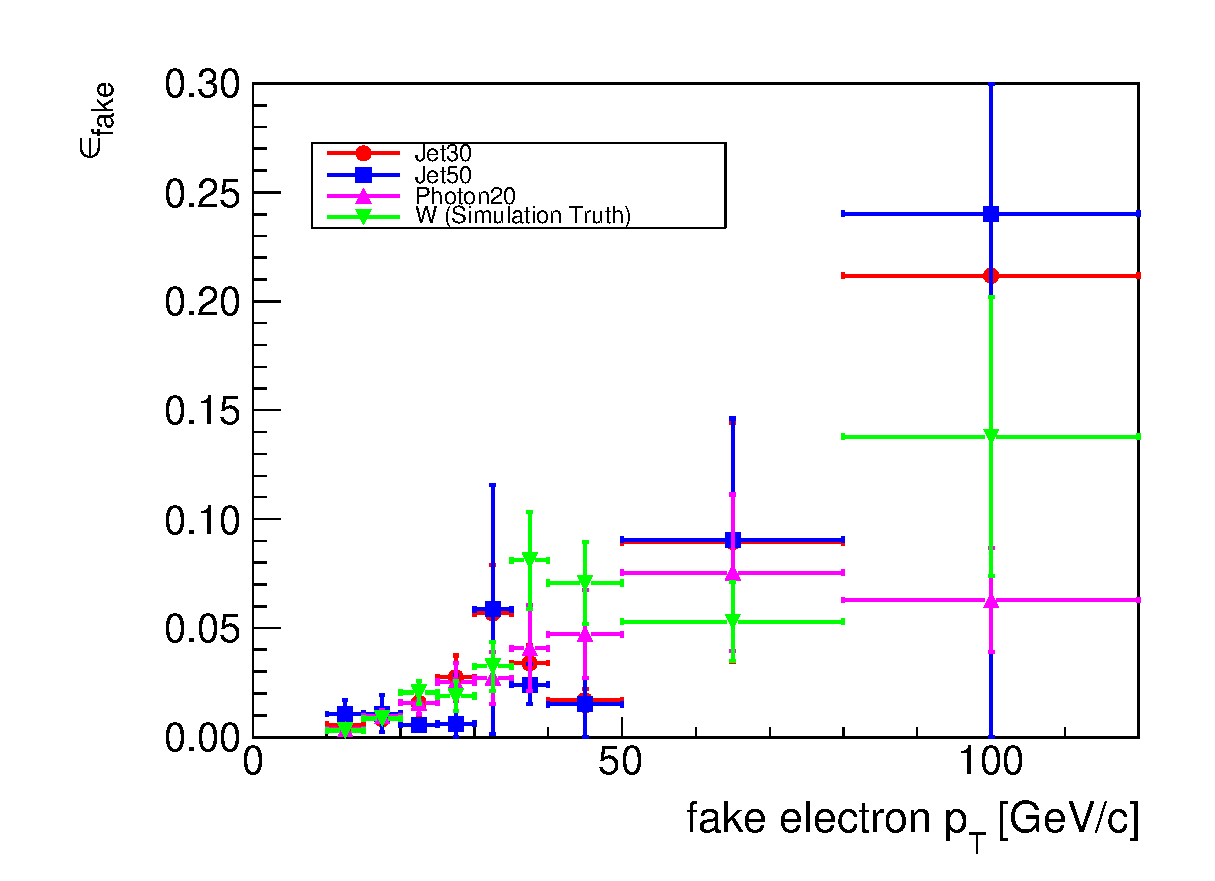
\includegraphics[width=0.49\textwidth]{plots/RecoElectronFakeRatePt.eps}} 
    \subfigure[]{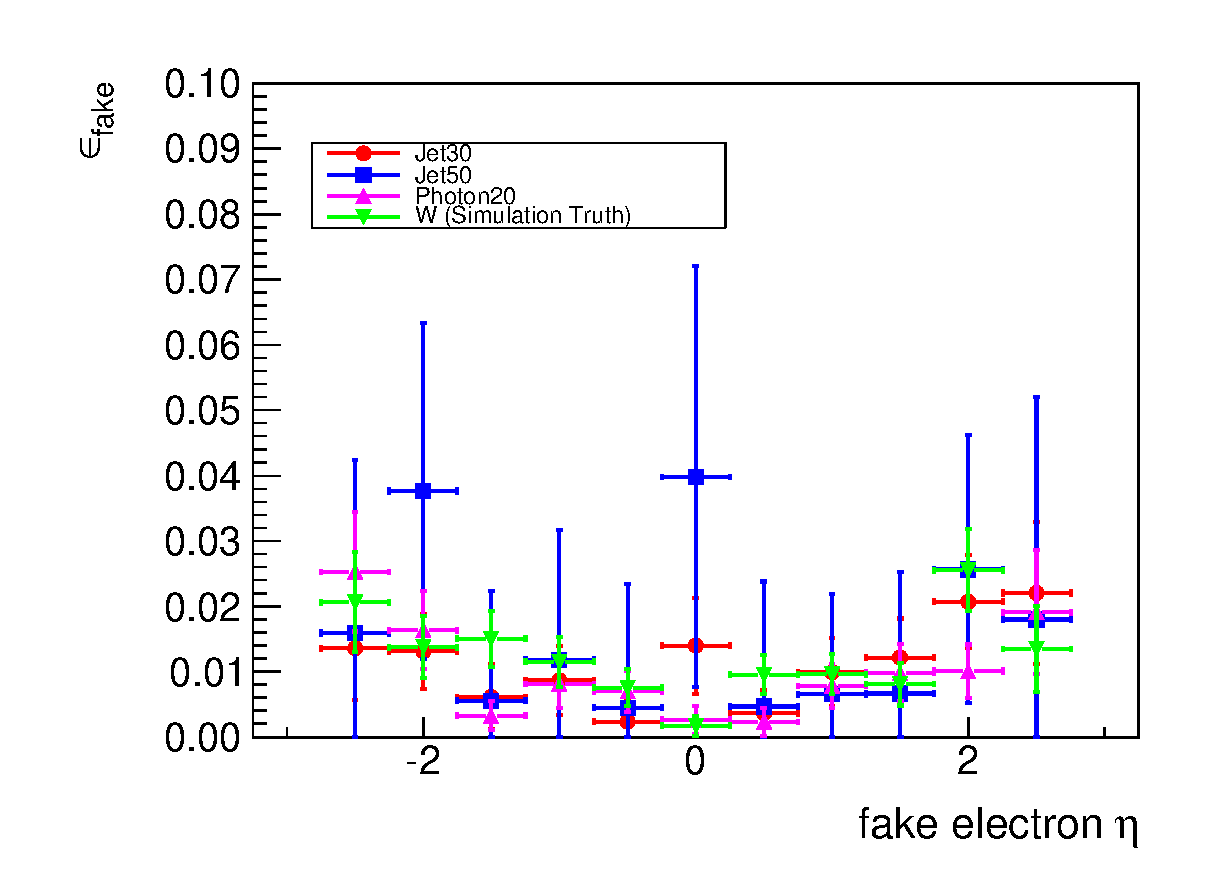
\includegraphics[width=0.49\textwidth]{plots/RecoElectronFakeRateEta.eps}}
    
    \caption{One-dimensional projections of the electron fake rate ($\epsilon_{fake}$) as a function of $p_{T}$ and $\eta$. Measurements in two jet trigger samples, one photon trigger sample, and the W+jet sample are shown. }
    \label{fig:electronFakeRate}
  \end{center}
\end{figure}

\begin{figure}[htb]
  \begin{center}
    \subfigure[]{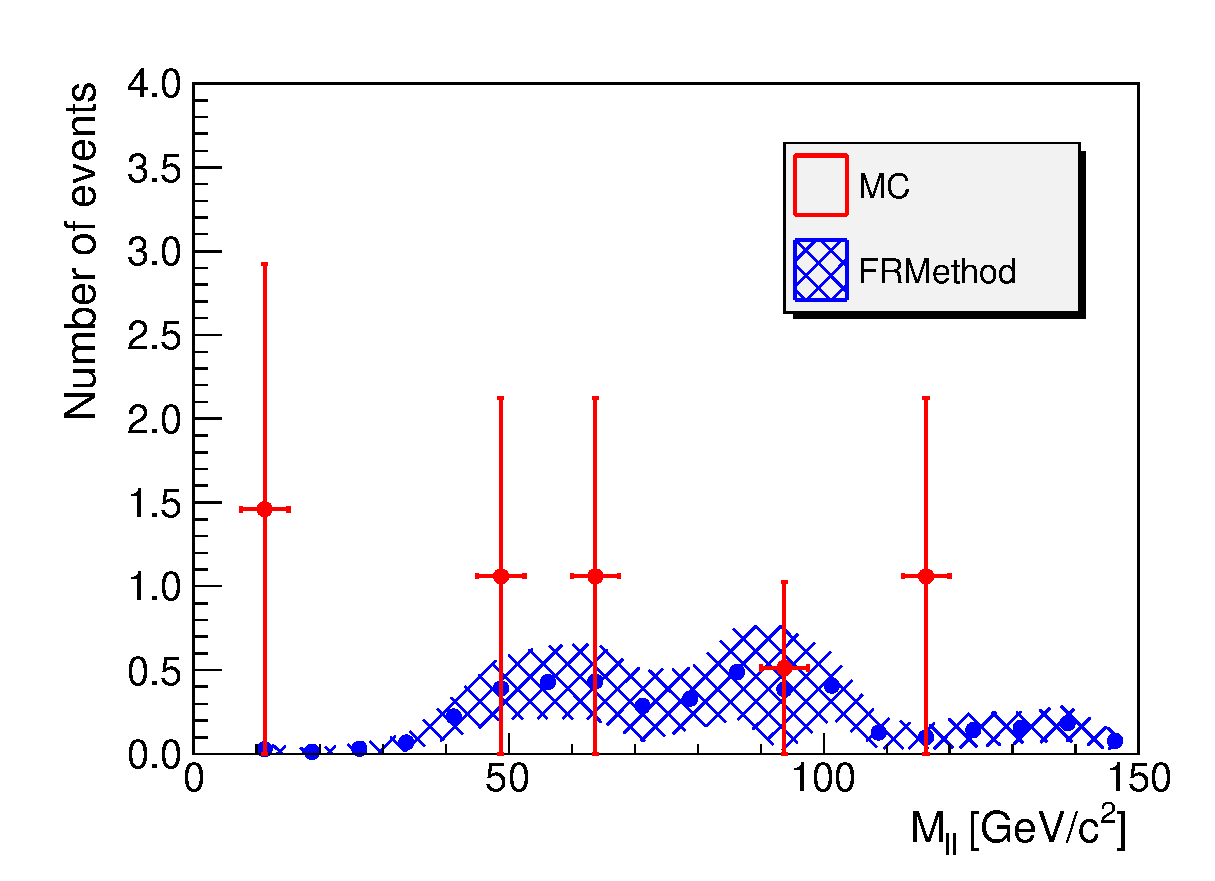
\includegraphics[width=0.49\textwidth]{plots/zeeDileptonMass_FakeRatePrediction_QCD.eps}}     
    \subfigure[]{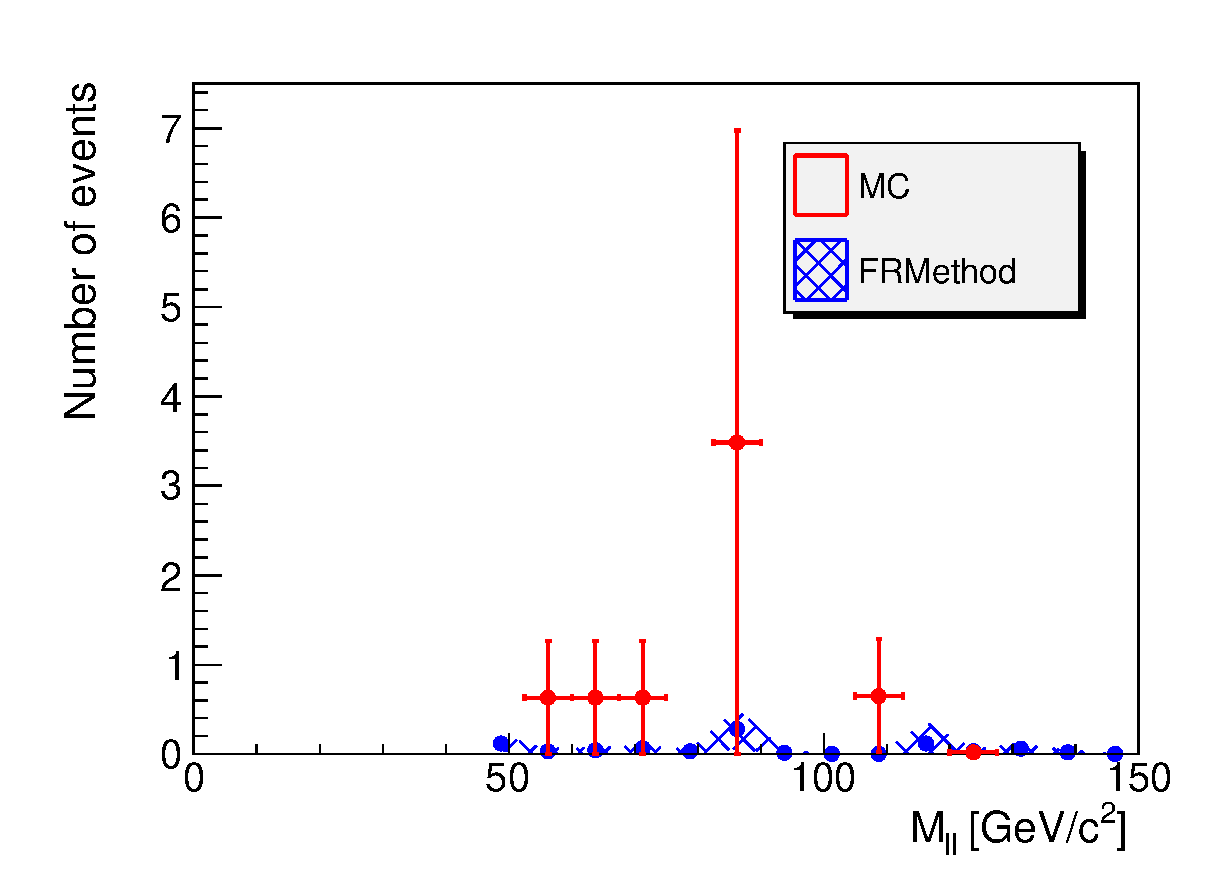
\includegraphics[width=0.49\textwidth]{plots/zeeDileptonMass_FakeRatePrediction_PhotonJets.eps}}     
    \subfigure[]{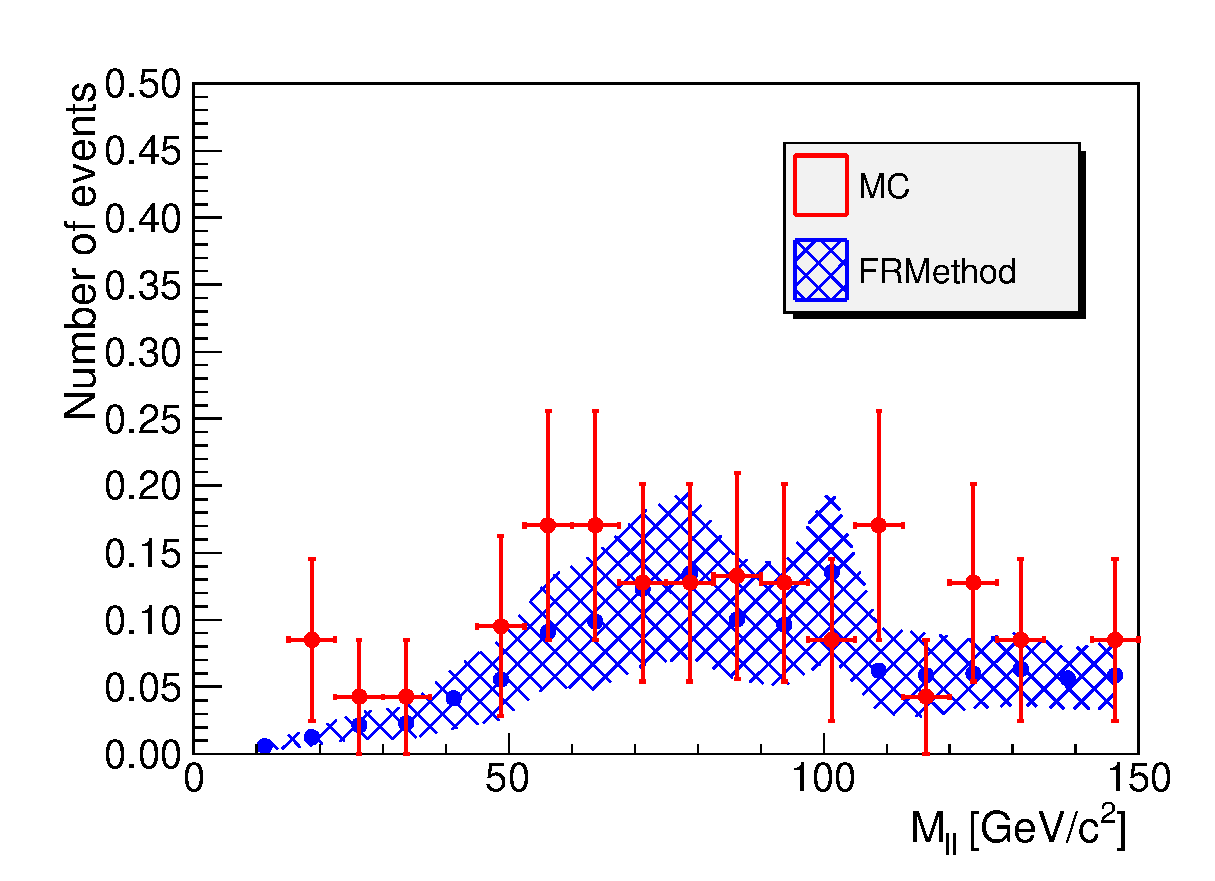
\includegraphics[width=0.49\textwidth]{plots/zeeDileptonMass_FakeRatePrediction_WJets.eps}}     
    \caption{A comparison of the dielectron mass distribution from the Monte Carlo simulation prediction and the prediction using the fake rate method, shown separately for the QCD multijet process (a), the $\gamma$+jets process (b), and the $\W+$jets process (c). The shaded region represents the estimated systematic uncertainties of the fake rate method prediction.}
    \label{fig:zeeDileptonMass_FakeRatePrediction}
  \end{center}
\end{figure}


\begin{figure}[htb]
  \begin{center}
    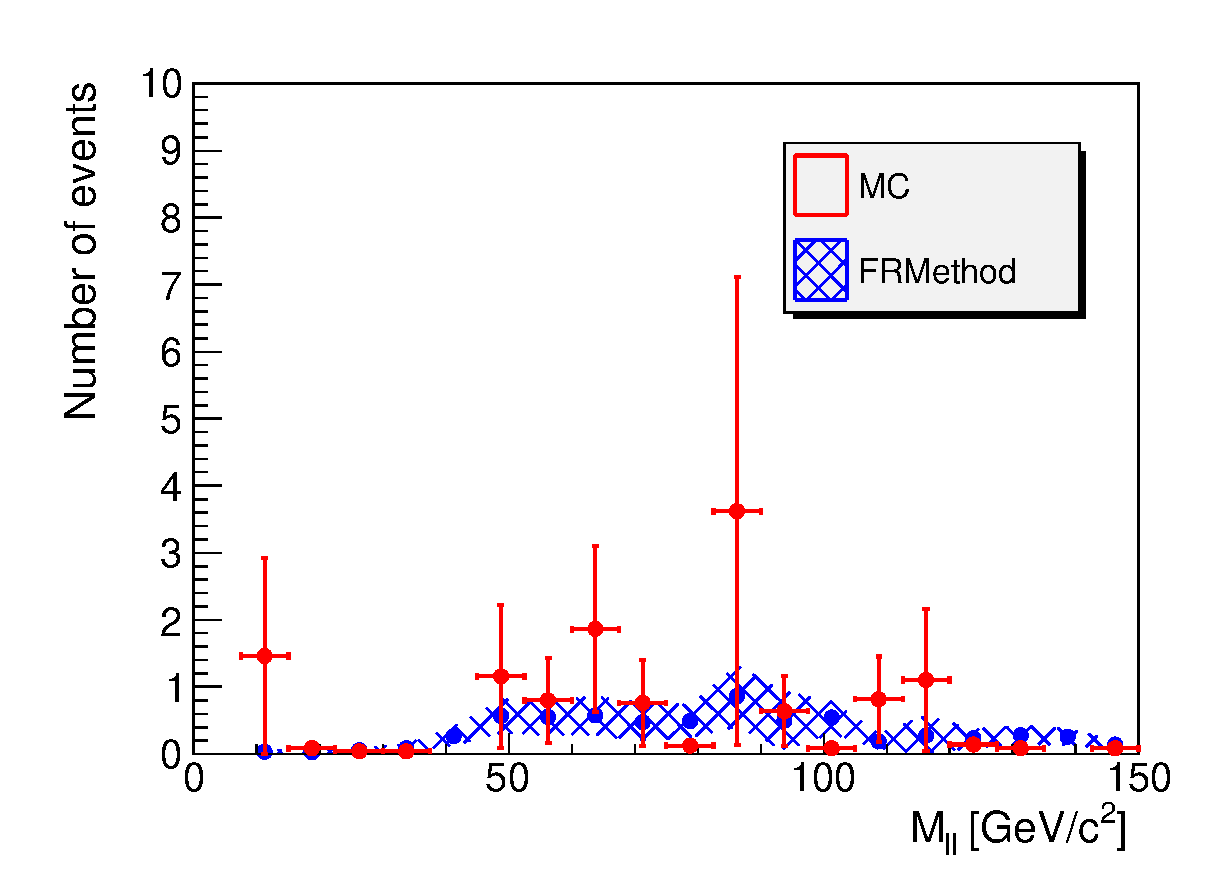
\includegraphics[width=0.49\textwidth]{plots/zeeDileptonMass_FakeRatePrediction_Total.eps}     
    \caption{A comparison of the dielectron mass distribution from the Monte Carlo simulation prediction and the prediction using the fake rate method for the sum of all fake lepton backgrounds. The shaded region represents the estimated systematic uncertainties of the fake rate method prediction. }
    \label{fig:zeeDileptonMass_FakeRatePrediction_Total}
  \end{center}
\end{figure}


The hadronic background prediction obtained using the fake rate method is summarized in Table \ref{tab:zeeHadBckFakeRateMethod}.

\begin{table}[!ht]
\begin{center}
\begin{tabular}{|c|c|c|}
\hline
 Process & Fake Rate Method Event Yield for $10\ \ipb$ & Monte Carlo Simulation Event Yield for $10\ \ipb$\\
\hline
\hline
 QCD multijet               & $2.6 \pm 1.7$ & $0.5 \pm 0.7$  \\
 $\gamma+$jet               & $0.7 \pm 0.8$ & $4.8 \pm 2.2$  \\
 W+jet                      & $0.7 \pm 0.8$ & $0.6 \pm 0.8$  \\

\hline
\end{tabular}
\caption{The hadronic background event yield for $10\ \ipb$ after all \Z\To\Ep\Em event selection cuts obtained using the same-sign background estimation technique compared with the event yield from the Monte Carlo simulation prediction.\label{tab:zeeHadBckFakeRateMethod}}
\end{center}
\end{table}


\customSection{Systematic Uncertainties}
\label{sec:systematics}
There are four main areas of systematic uncertainties for this measurement, resulting from the four main components of this analysis. The uncertainties come from the integrated luminosity measurement, the detector acceptance of the $\Z$ boson signal events, the measurement of the event selection efficiencies, and the estimate of the background contribution. Each component will be discussed separately below.

\customSubsection{Luminosity Measurement}
The luminosity measurement for this analysis is primarily obtained from the first measurements performed by the LHC machine. Current estimates of the uncertainty of this measurement show a large variation, ranging from $10\%$ to $20\%$.

\customSubsection{Signal Acceptance}
\label{sec:pdfSystematic}
There are a number of theoretical aspects related to the production of a $\Z$ boson in proton-proton collisions that have inherent uncertainties. All of these uncertainties affect the prediction for the number of $\Z$ boson events that are produced and their kinematic properties. Due to the effect of limited geometric acceptance of the detector apparatus, these uncertainties lead to uncertainties on the cross section measurement. Furthermore, since the signal acceptance must be obtained from Monte Carlo simulation, there are certain experimental uncertainties that are not necessarily modelled perfectly in the detector simulation, which also affect the cross section measurement. These effects will be described in detail below.

\customSubsubsection{Parton Distribution Function Model}
The momentum distribution of quarks and gluons inside the proton are modelled by parton distribution functions obtained from fits to previous experimental data. There are inherent uncertainties to these PDF sets from theoretical uncertainties and the uncertainties from the input measurements. These functions are used as inputs to the Monte Carlo simulation and a change in their parameters lead to changes in the kinematics predicted for the $\Z$ boson event. In particular, the choice of a PDF has a significant effect on the shape of the $\Z$ boson rapidity distribution, which in turn has an effect on the signal acceptance. 

In order to estimate the systematic uncertainty due to the choice of a PDF, we select the set of PDF's which have $1\sigma$ high or low fluctuations of the diagonalized parameters. For each such variation, we compare the difference in the signal acceptance to the default median PDF provided. For this study, events are generated using the NLO event generator POWHEG with the NLO parton distribution function set CTEQ66. In the case of a leading order event generator using a leading order parton distribution function, the PDF systematic uncertainty can be studied by using a reweighting procedure, since the differential cross section is linear in the parton distribution function values. In the next-to-leading-order case, the situation is made more complex by the presence of higher order terms that are no longer linear in the parton distribution functions. To study the magnitude of the effect of the non-linear terms we compare the acceptance values obtained using the reweighting method and those obtained from separate Monte Carlo samples produced using the different parton distribution functions of the CTEQ66 PDF set. 

We begin by briefly summarizing the PDF reweighting method. Given a Monte Carlo sample generated using the best fit parton distribution function of a particular PDF set, $f_{0}(x,Q)$, we obtain a set of weights $w_{k}$ intended to match the kinematic behavior of a Monte Carlo sample generated using another PDF in the set, $f_{k}(x,Q)$, through the following relation:

\begin{eqnarray}
  w^{i}_{k} = \frac{f^{a_{i}}_{k}(x^{i}_{1},Q^{i})f^{b_{i}}_{k}(x^{i}_{2},Q^{i})}{f^{a_{i}}_{0}(x^{i}_{1},Q^{i})f^{b_{i}}_{0}(x^{i}_{2},Q^{i})}
  \label{eqn:PDFReweighting}  
\end{eqnarray}

where  $a_{i}$ is the flavor of the first parton, $b_{i}$ is the flavor of the second parton, and the $i$'s label the events. Kinematic distributions and the acceptance corresponding to the k'th PDF is computed using the same events with the set of weights $w_{k}$. The acceptance for the each PDF is compared to the acceptance for the nominal PDF. An asymetric systematic uncertainty is obtained by adding all the positive deviations from the nominal PDF in quadrature for the positive systematic uncertainty, and all the negative deviations from the nominal PDF in quadrature for the negative systematic uncertainty. 

Figure \ref{fig:PDFSystematicsReweightingMethod} summarizes the comparison between the acceptances computed using the reweighting method described above, and the acceptances computed from entirely different Monte Carlo samples produced using the different PDF's of the CTEQ66 set and the MSTW2008 set. We observe that for the majority of PDF's in the CTEQ66 set, the deviation between the acceptance computed using the reweighting method and the acceptance computed from the Monte Carlo sample produced using that PDF is less than $0.1\%$. Only a handful of PDF's exhibit deviation on the order of $0.1\%$. However, we note that the acceptances computed using the reweighting method is smaller than the acceptances computed from the generated Monte Carlo samples for a number of PDF's. This results in systematic uncertainties which are larger in the positive direction than the negative direction when the actual Monte Carlo samples are used. The differences in the acceptance calcualted from the different members of the MSTW2008 PDF set is significantly less than the differences in the acceptances calculated from the CTEQ66 set. To summarize, for the CTEQ66 PDF set, the reweighting method yields asymmetric systematic uncertainties of $^{+1.4 \%}_{- 1.4 \%}$ , while the actual Monte Carlo samples yield systematic uncertainties of $^{+1.7 \%}_{- 1.3 \%}$.  For the MSTW2008 PDF set, we observe systematic uncertainties of $^{+0.5 \%}_{- 0.4 \%}$ using the reweighting method, and $^{+0.6 \%}_{- 0.6 \%}$ using the consistently generated Monte Carlo samples. Finally, the acceptance calculated from the best fit PDF of the CTEQ66 set is $0.3\%$ lower than the acceptance calculated from the best fit PDF of the MSTW2008 set.


\begin{figure}[htb]
  \begin{center}
    \subfigure[]{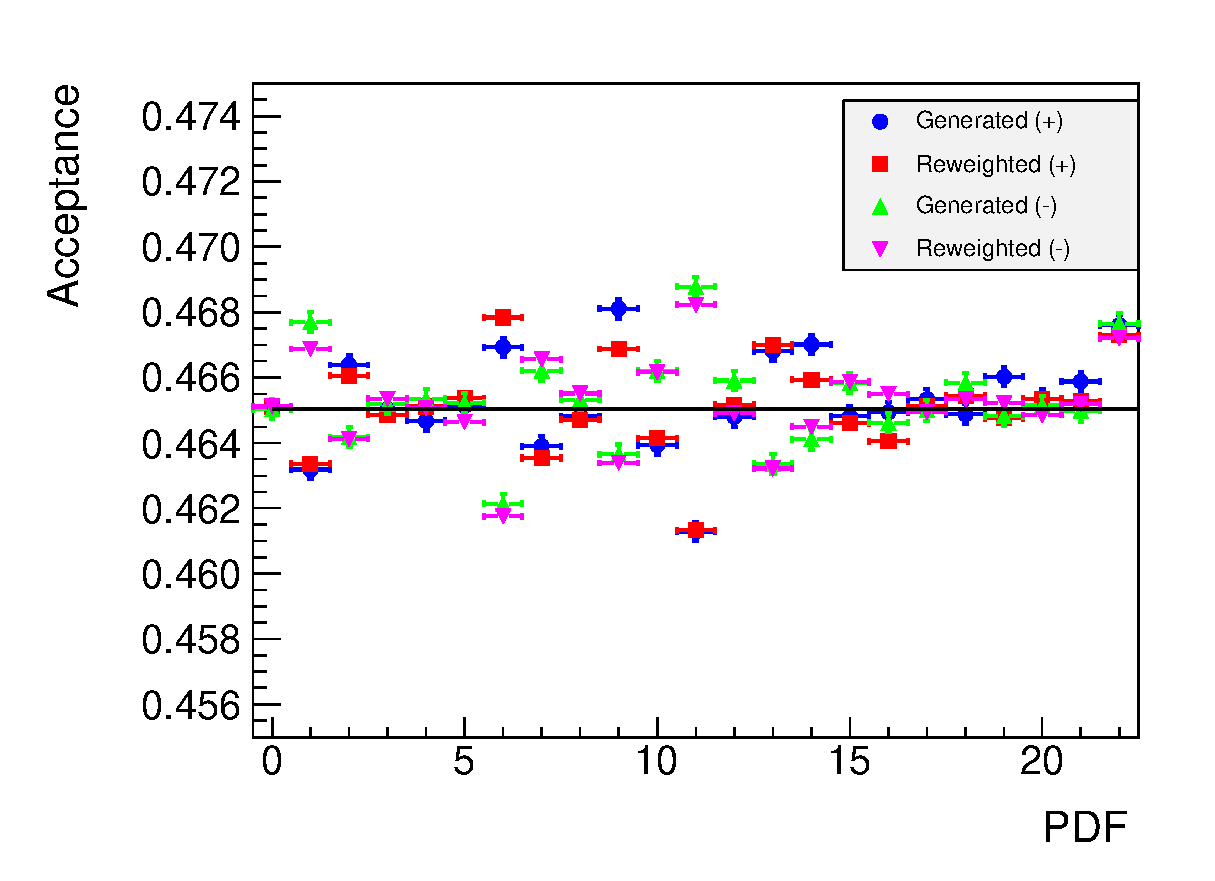
\includegraphics[width=0.49\textwidth]{plots/PDFSystematics_ReweightVsGenerate_CTEQ66.eps}} 
    \subfigure[]{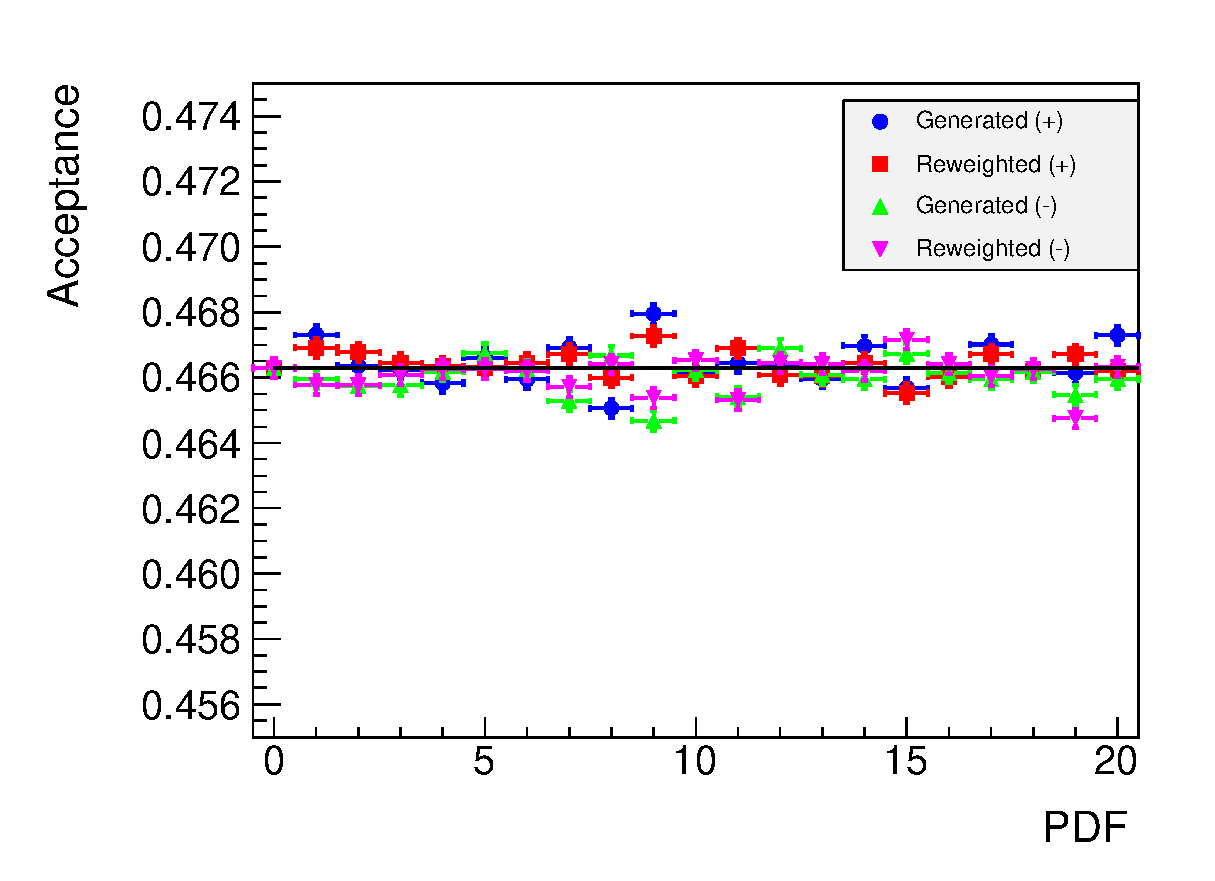
\includegraphics[width=0.49\textwidth]{plots/PDFSystematics_ReweightVsGenerate_MSTW2008.eps}}     
    %This one shows fractional differences to the nominal PDF
    %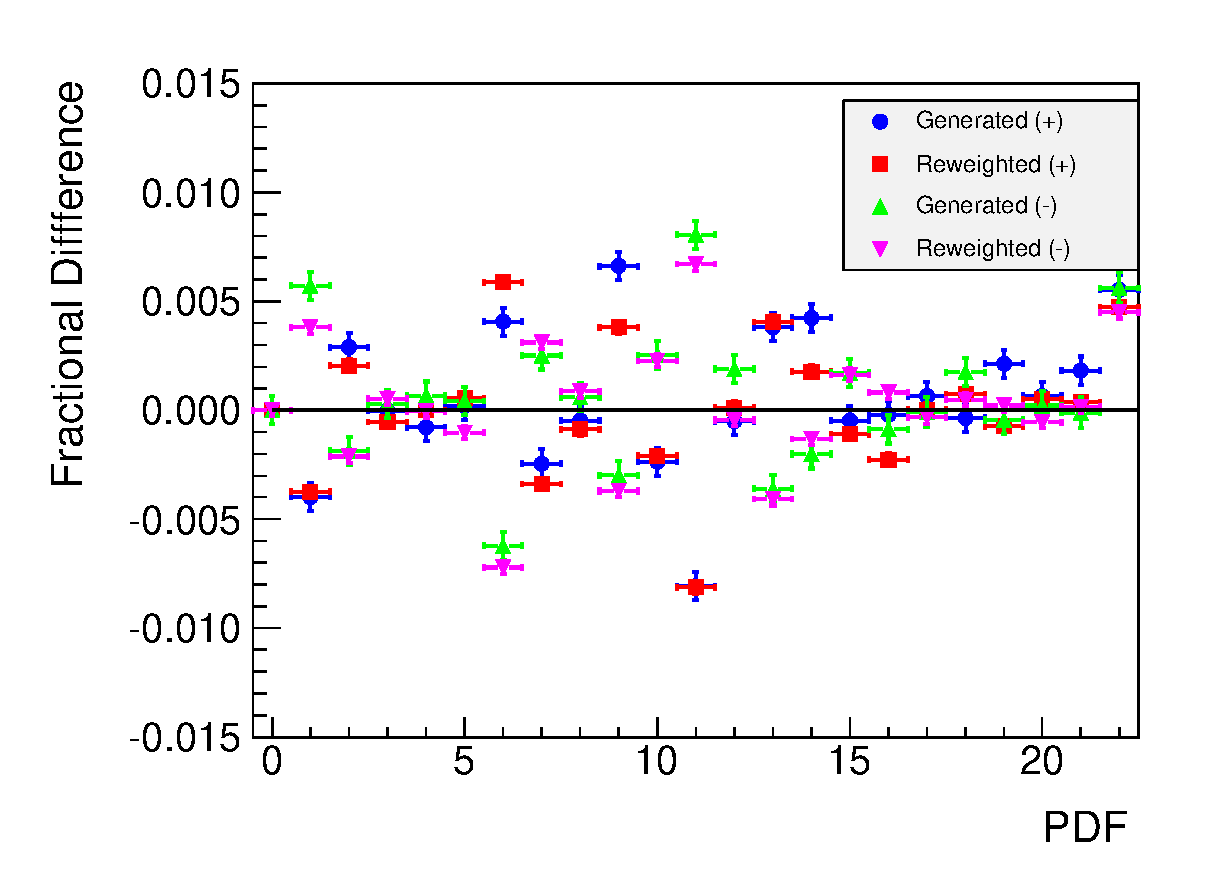
\includegraphics[width=0.60\textwidth]{plots/PDFSystematics_ReweightVsGenerate_FractionalDifferences_CTEQ66.eps}  
    %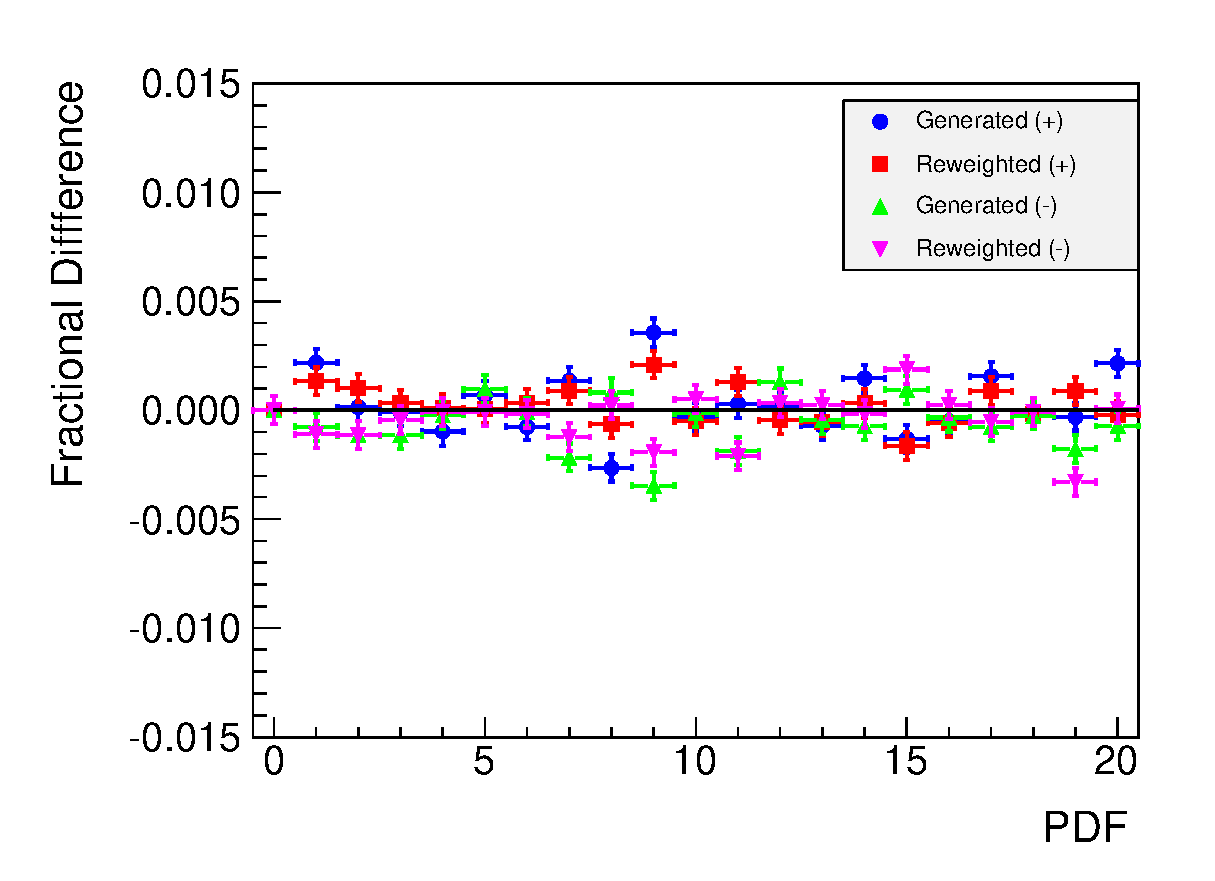
\includegraphics[width=0.60\textwidth]{plots/PDFSystematics_ReweightVsGenerate_FractionalDifferences_MSTW2008.eps}  
    \caption{A comparison of the acceptances computed using the reweighting method and the acceptances from separately generated Monte Carlo samples using each of the individual PDFs in the CTEQ66 (a) and MSTW2008 $68\%$ confidence level (b) PDF sets. The acceptance values are separated into PDF's with positive variation of the PDF parameter (+) and negative variation of the PDF parameter (-). The acceptance values computed using the reweighting method are shown in blue and green, for the positive and negative variations respectively, while the acceptance values computed from the separately generated Monte Carlo samples are shown in red and magenta, for the positive and negative variations respectively. The acceptance computed using the best fit PDF is shown in the black line. }
    \label{fig:PDFSystematicsReweightingMethod}
  \end{center}
\end{figure}

In order to account for possible effects of reconstruction and detector resolution on the kinematic differences due to different parton distribution functions, it is desirable to estimate the systematic uncertainty using fully reconstructed objects and applying the full event selection. Therefore, for the final systematic uncertainty estimate, we evaluate the effect of the PDF fit parameter variation on the full event selection efficiency defined to be the acceptance multiplied by the object reconstruction efficiencies and the event selection cut efficiencies. Figure \ref{fig:PDFSystematicsFullEventSelection} shows a comparison of the fractional difference in the full event selection efficiency relative to the best fit PDF, and the fractional difference in the generator level acceptance relative to the best fit PDF for each of the PDFs in the CTEQ66 set in events generated using POWHEG, and computed using the reweighting method. The Monte Carlo sample is not completely compatible since the only full simulation sample available was one generated using the CTEQ6M PDF and showered using the CTEQ6L PDF. Nevertheless, we see that the differences between the acceptance level systematic uncertainties and the full event selection level systematic uncertainties are less than $0.1\%$. The asymmetric systematic uncertainty obtained using the full event selection efficiency is $^{+1.5\%}_{-1.5\%}$, while by comparison the asymmetric systematic uncertainty calculated using the generator level acceptance is $^{+1.4\%}_{-1.4\%}$, for the sample sample of events.

\begin{figure}[htb]
  \begin{center}
    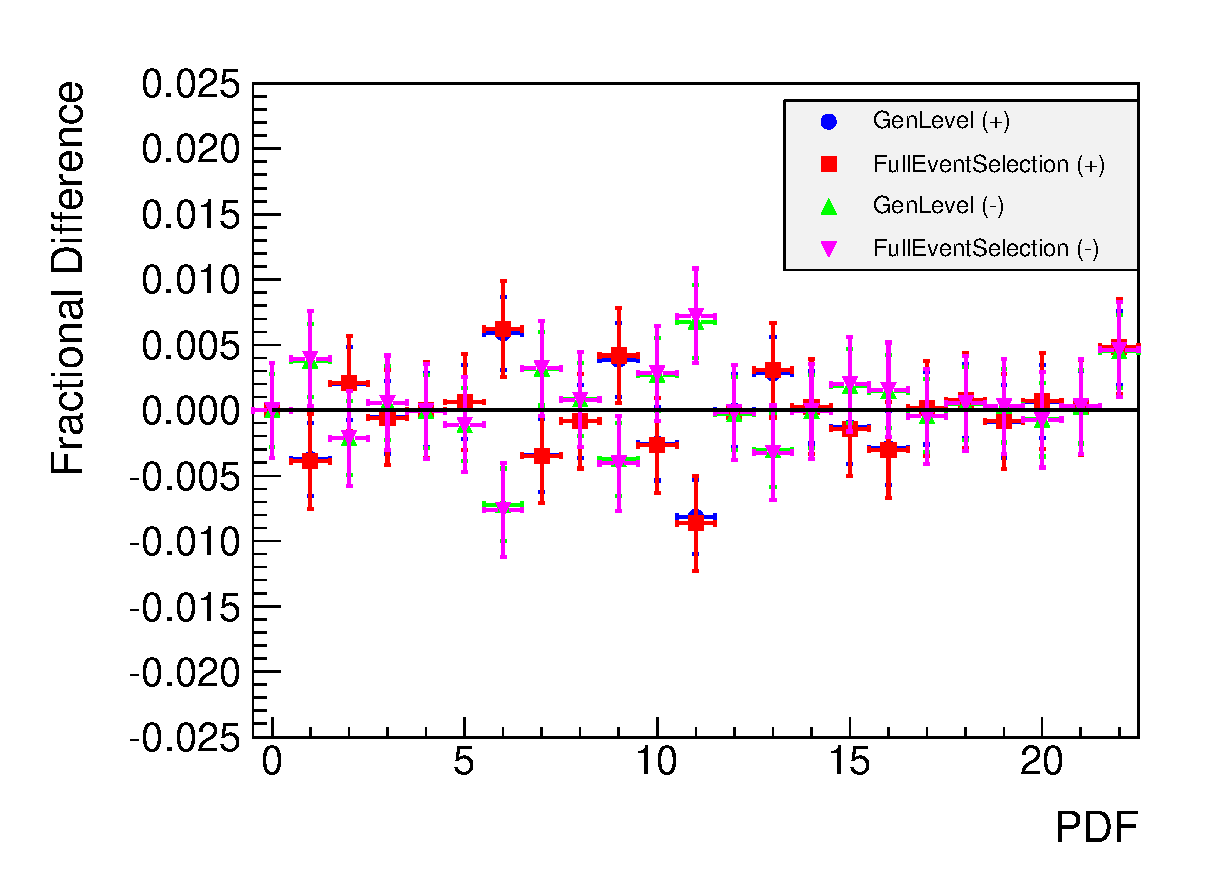
\includegraphics[width=0.60\textwidth]{plots/PDFSystematics_GenLevelVsFullEventSelection_CTEQ66_s09-zeem20-7-mc3.eps} 
    \caption{A comparison of the fractional differences in the acceptance computed at generator acceptance level, shown in blue and green, and the efficiency of the full event selection, shown in red and magenta, for each of the PDF's in the PDF set using the reweighting method relative to the best fit PDF. }
    \label{fig:PDFSystematicsFullEventSelection}
  \end{center}
\end{figure}


In the future, the final systematic uncertainty should be computed using a fully simulated POWHEG Monte Carlo sample produced and showered using the CTEQ66 PDF. Ideally, one should perform the study by generating separate samples for each of the PDF's in the PDF set, however this requires too much computational resources if it is done at the full simulation level. One can, instead, correct the systematic uncertainties calculated at full events selection level by the difference between the reweighting method and the separately generated result at generator acceptance given in Figure \ref{fig:PDFSystematicsReweightingMethod}, where an implicit assumption is made that the differences observed at the generator acceptance level largely propagates through to the full event selection level. 



\customSubsubsection{Higher Order QCD and Electroweak Corrections}
Next-to-leading order (NLO) and next-to-next-to-leading order (NNLO) perturbative QCD corrections, as well as soft non-perturbative QCD corrections can have a significant effect on the rapidity and transverse momentum of the $\Z$ bosons produced. Electroweak NLO corrections can have significant effects on the rate of final state radiation which affects the transverse momentum distribution of the leptons. All of these corrections can have significant effects on the acceptance for $\Z$ boson events. The results of similar studies for the W boson can be found in reference \cite{HigherOrderQCDSystematicsForW}.

To evaluate the effect of the soft non-perturbative QCD corrections, we compare the acceptance evaluated using the Resbos program\cite{Resbos}, an integrator program which uses a resummation procedure accurate to next-to-next-to-leading-log order, to the acceptance evaluated using a full NLO event generator POWHEG\cite{Powheg} interfaced with PYTHIA. Figure \ref{fig:ResbosVsPowheg_ZRapidityPt} shows a comparison of the $\Z$ boson rapidity distribution and the $\Z$ boson transverse momentum distribution predicted by Resbos and POWHEG. Figure \ref{fig:ResbosVsPowheg_LeptonRapidityPt} shows the analogous comparison for the transverse momentum and rapidity distribution of the leptons resulting from the $\Z$ boson decay. The fractional difference in the acceptance computed using Resbos and the acceptance computed using POWHEG is shown to be $0.6\%$. Without a study of the relevent distributions in data, this represents the current best estimate of the systematic uncertainty due to soft non-perturbative QCD effects.

%% \begin{figure}[htb]
%%   \begin{center}
%%     \subfigure[]{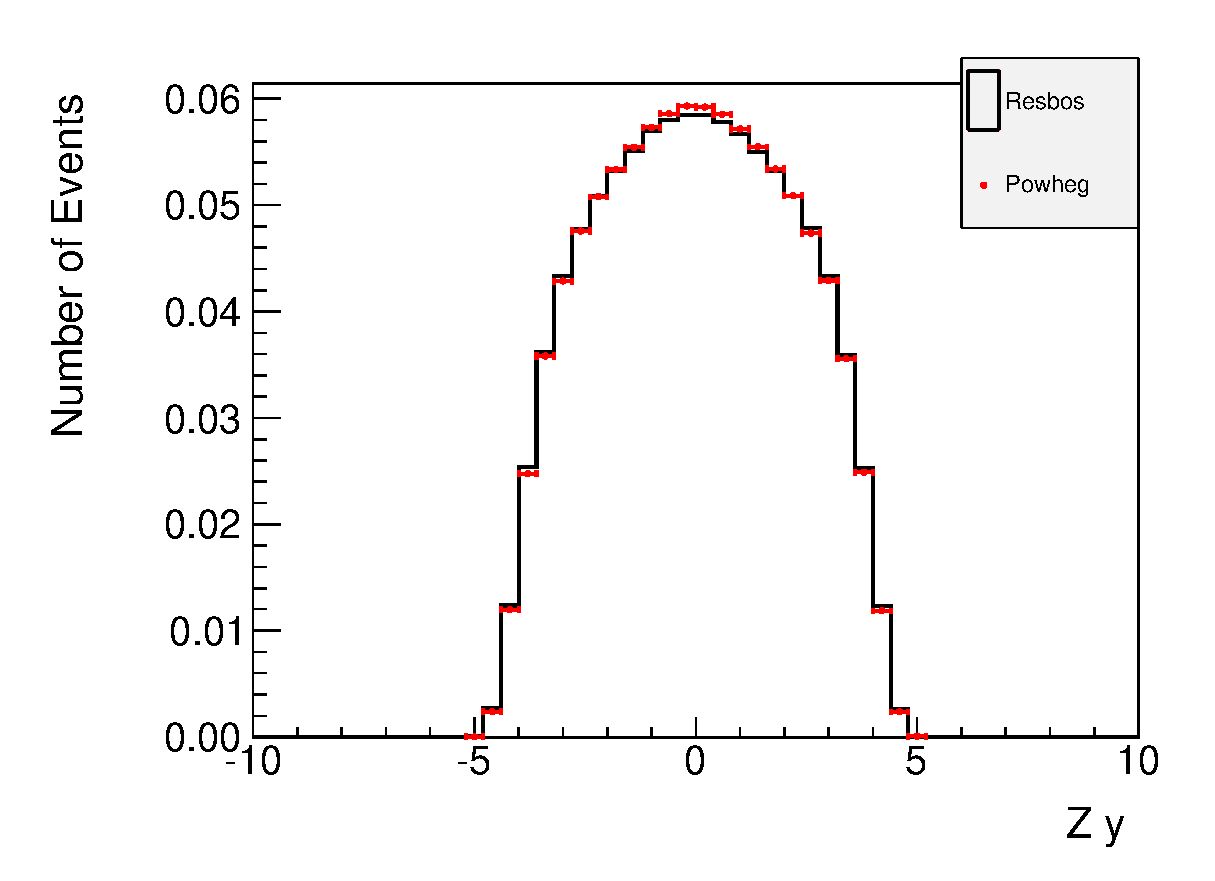
\includegraphics[width=0.49\textwidth]{plots/ZRapidity_ResbosVsPowheg_14TeV.eps}} 
%%     \subfigure[]{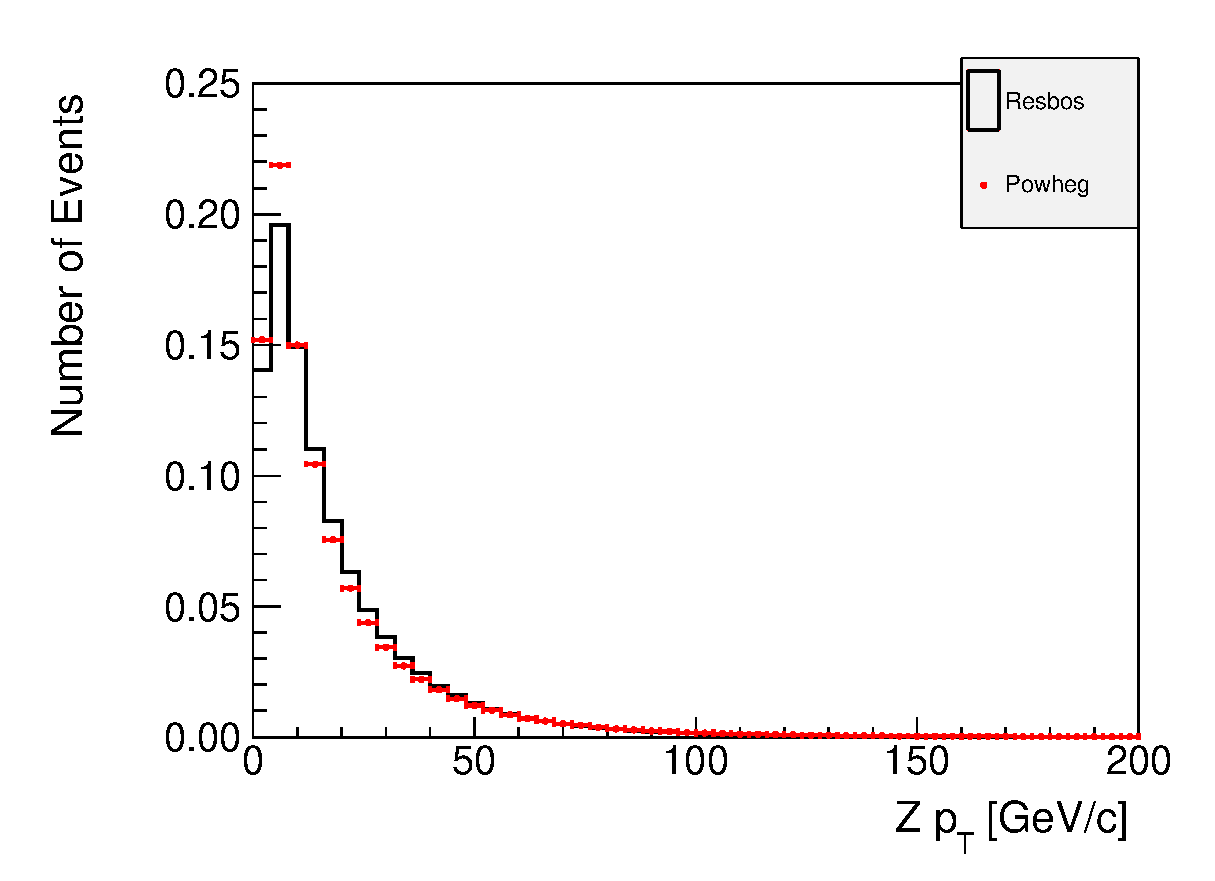
\includegraphics[width=0.49\textwidth]{plots/ZPt_ResbosVsPowheg_14TeV.eps}} 
%%     \subfigure[]{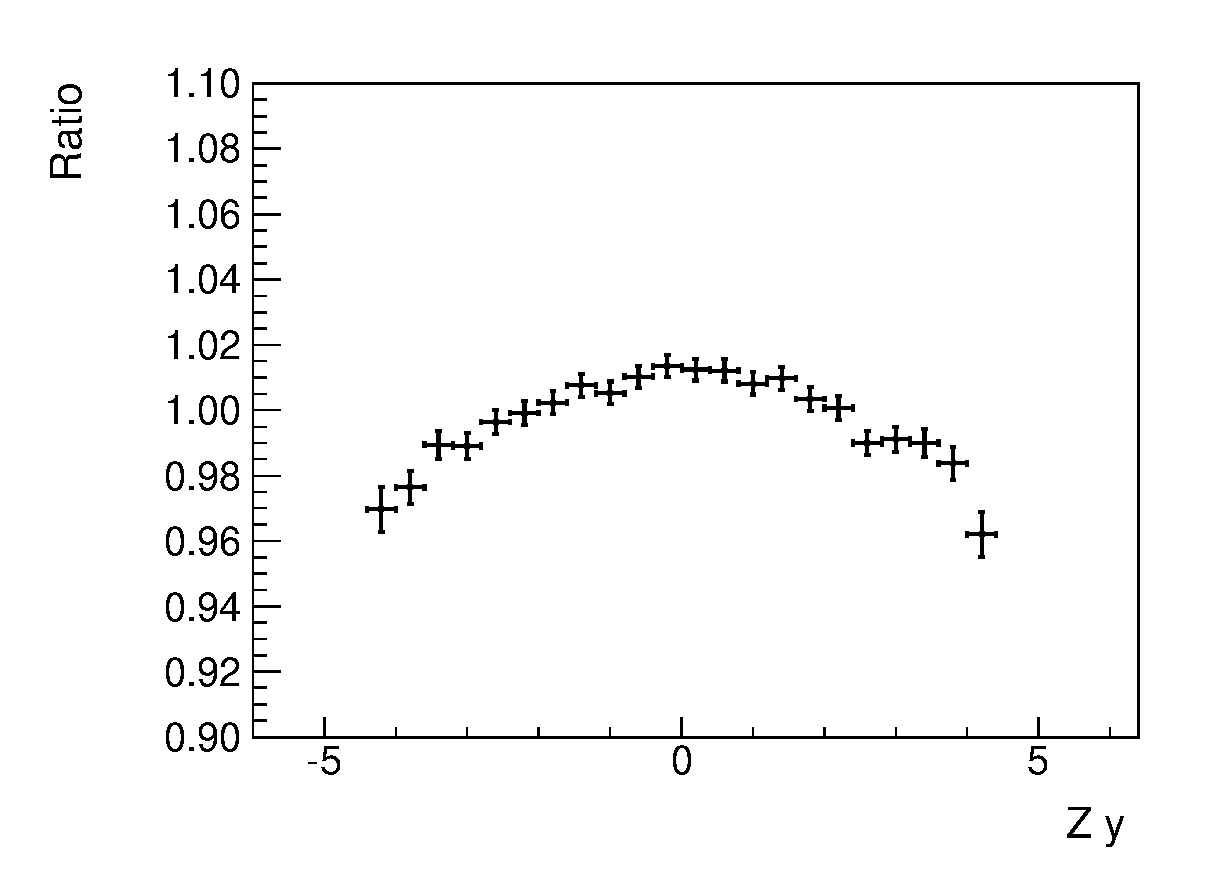
\includegraphics[width=0.49\textwidth]{plots/ZRapidityRatio_ResbosVsPowheg_14TeV.eps}} 
%%     \subfigure[]{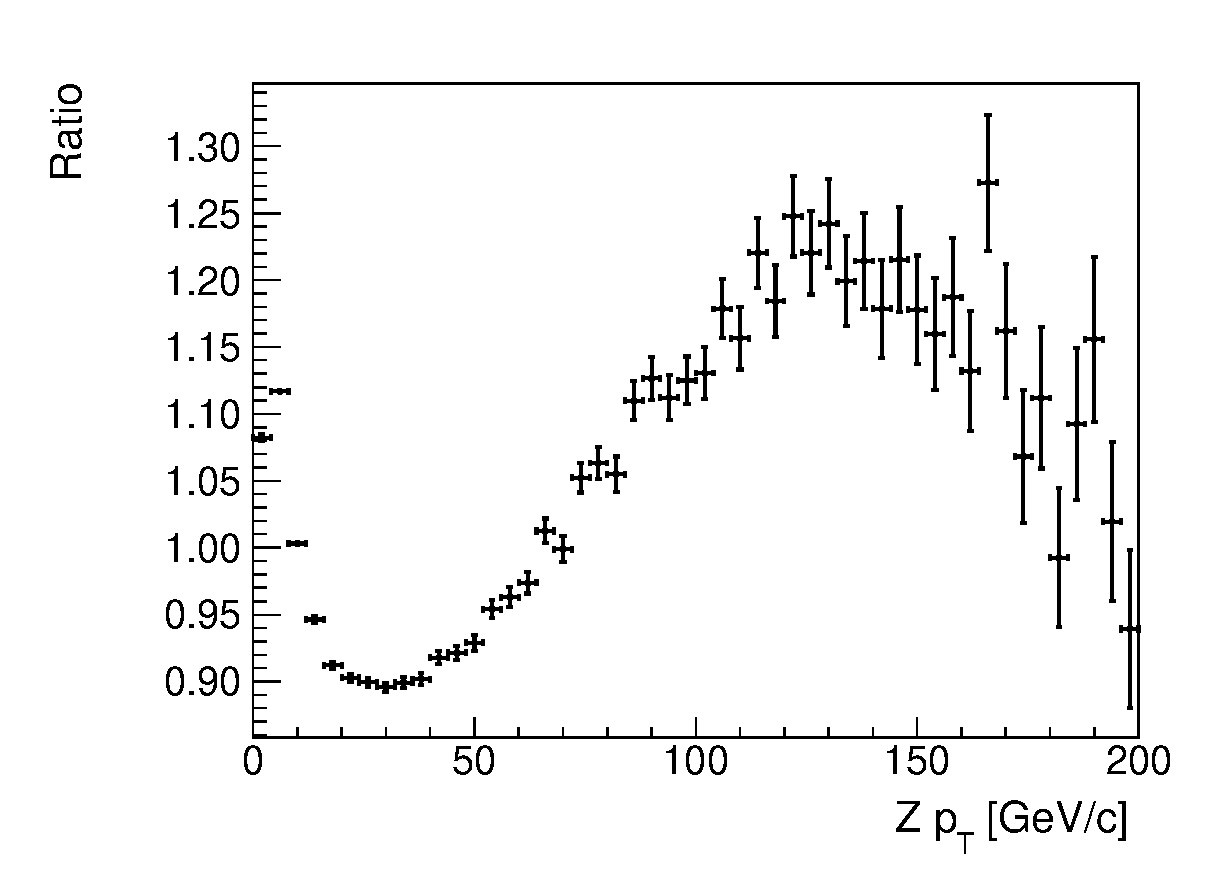
\includegraphics[width=0.49\textwidth]{plots/ZPtRatio_ResbosVsPowheg_14TeV.eps}} 
%%     \caption{A comparison of the rapidity (a) and transverse momentum (b) distributions of the $\Z$ boson produced by Resbos and POWHEG. The ratio of POWHEG prediction to the Resbos prediction is shown in (c) for the $\Z$ boson rapidity, and in (d) for the $\Z$ boson transverse momentum.}
%%     \label{fig:ResbosVsPowheg_ZRapidityPt}
%%   \end{center}
%% \end{figure}

%% \begin{figure}[htb]
%%   \begin{center}
%%     \subfigure[]{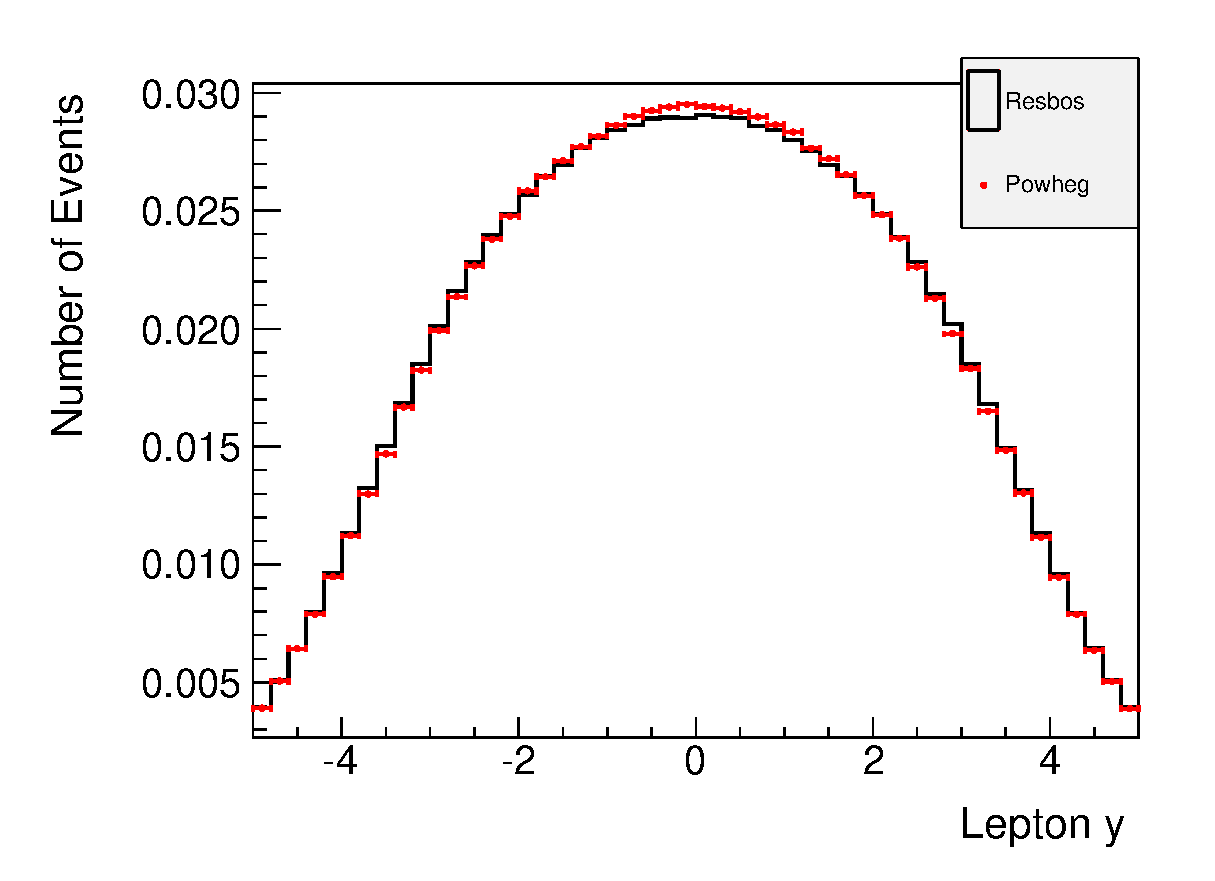
\includegraphics[width=0.49\textwidth]{plots/Lepton1Y_ResbosVsPowheg_14TeV.eps}} 
%%     \subfigure[]{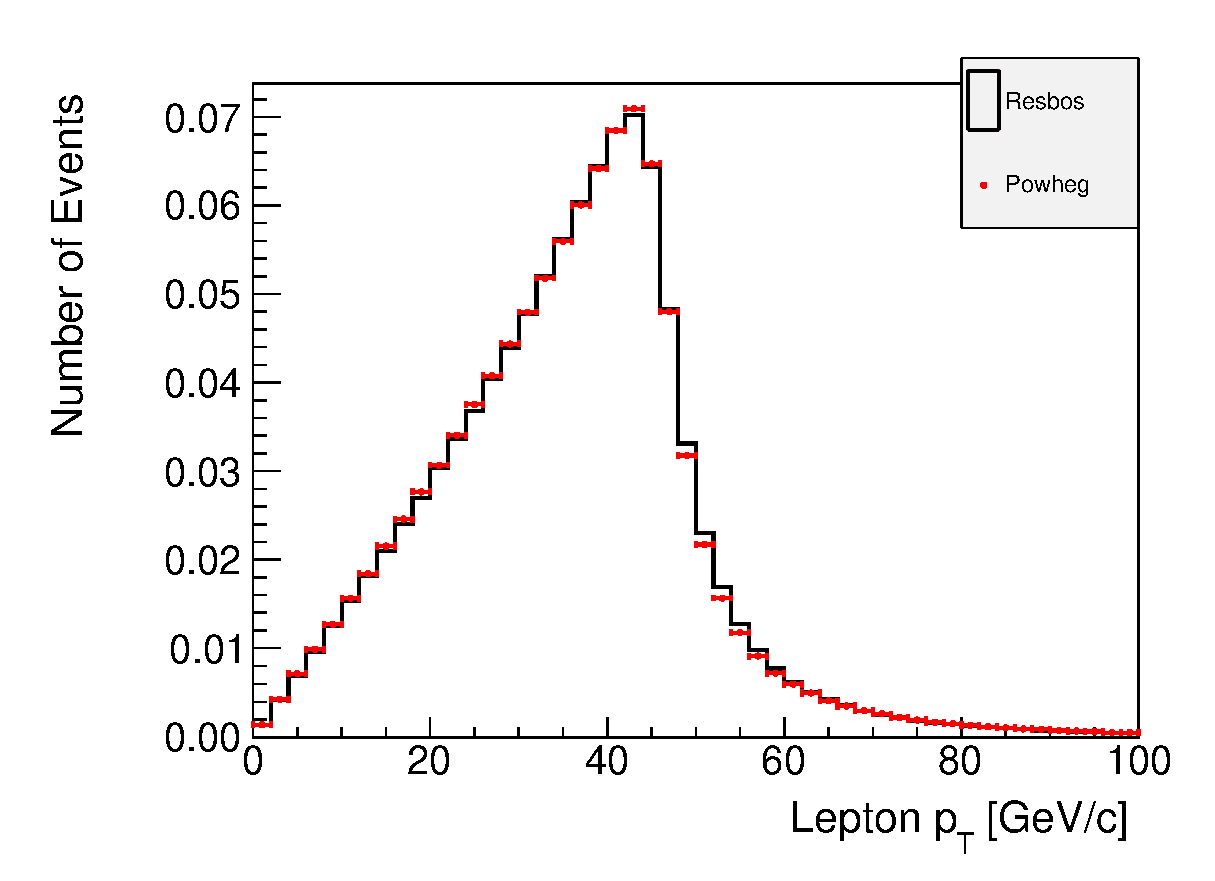
\includegraphics[width=0.49\textwidth]{plots/Lepton1Pt_ResbosVsPowheg_14TeV.eps}} 
%%     \subfigure[]{\includegraphics[width=0.49\textwidth]{plots/ZLepton1YRatio_ResbosVsPowheg_14TeV.eps}} 
%%     \subfigure[]{\includegraphics[width=0.49\textwidth]{plots/ZLepton1PtRatio_ResbosVsPowheg_14TeV.eps}} 
%%     \caption{A comparison of the rapidity (a) and transverse momentum (b) distributions of the leptons from the $\Z$ boson decay as predicted by Resbos and POWHEG. The ratio of the POWHEG prediction to the Resbos prediction is shown in (c) for the lepton rapidity, and in (d) for the lepton transverse momentum.}
%%     \label{fig:ResbosVsPowheg_LeptonRapidityPt}
%%   \end{center}
%% \end{figure}

\begin{figure}[htb]
  \begin{center}
    \subfigure[]{\includegraphics[width=0.49\textwidth]{plots/ZRapidity_ResbosVsPowheg_7TeV.eps}} 
    \subfigure[]{\includegraphics[width=0.49\textwidth]{plots/ZPt_ResbosVsPowheg_7TeV.eps}} 
    \subfigure[]{\includegraphics[width=0.49\textwidth]{plots/ZRapidityRatio_ResbosVsPowheg_7TeV.eps}} 
    \subfigure[]{\includegraphics[width=0.49\textwidth]{plots/ZPtRatio_ResbosVsPowheg_7TeV.eps}} 
    \caption{A comparison of the rapidity (a) and transverse momentum (b) distributions of the $\Z$ boson produced by Resbos and POWHEG. The ratio of POWHEG prediction to the Resbos prediction is shown in (c) for the $\Z$ boson rapidity, and in (d) for the $\Z$ boson transverse momentum.}
    \label{fig:ResbosVsPowheg_ZRapidityPt}
  \end{center}
\end{figure}

\begin{figure}[htb]
  \begin{center}
    \subfigure[]{\includegraphics[width=0.49\textwidth]{plots/Lepton1Y_ResbosVsPowheg_7TeV.eps}} 
    \subfigure[]{\includegraphics[width=0.49\textwidth]{plots/Lepton1Pt_ResbosVsPowheg_7TeV.eps}} 
    \subfigure[]{\includegraphics[width=0.49\textwidth]{plots/ZLepton1YRatio_ResbosVsPowheg_7TeV.eps}} 
    \subfigure[]{\includegraphics[width=0.49\textwidth]{plots/ZLepton1PtRatio_ResbosVsPowheg_7TeV.eps}} 
    \caption{A comparison of the rapidity (a) and transverse momentum (b) distributions of the leptons from the $\Z$ boson decay as predicted by Resbos and POWHEG. The ratio of the POWHEG prediction to the Resbos prediction is shown in (c) for the lepton rapidity, and in (d) for the lepton transverse momentum.}
    \label{fig:ResbosVsPowheg_LeptonRapidityPt}
  \end{center}
\end{figure}



The systematic uncertainties due to perturbative higher order QCD corrections can be evaluated by varying the renormalization and factorization scale of a particular process and computing the differences observed in the final event selection efficiency. Due to the high computational demand of the detector simulation, we perform this study at the generator acceptance level. Two different approaches are pursued. In the first approach we produce Monte Carlo samples using POWHEG where the factorization scale and renormalization set has been set to $2\times M_{\mathrm{Z}}$ and $M_{\mathrm{Z}}/2$ and evaluate the difference in the acceptance computed using these two samples. Figure \ref{fig:PowhegScaleVariation_ZRapidityPt} compares the rapidity and transverse momentum distribution of the $\Z$ boson for the two scale variations and the reference. Figure \ref{fig:PowhegScaleVariation_LeptonRapidityPt} shows the analogous comparison for the rapidity and transverse momentum distribution of one of the leptons in the $\Z$ boson decay. The acceptances and the fractional differences for this scale variation is summarized in Table \ref{tab:PowhegScaleVariation}. The systematic uncertainty due to this effect is $0.3\%$. 

\begin{figure}[htb]
  \begin{center}
    %\subfigure[]{\includegraphics[width=0.49\textwidth]{plots/ZRapidity_Powheg_ScaleVariation_7TeV.eps}} 
    %\subfigure[]{\includegraphics[width=0.49\textwidth]{plots/ZPt_Powheg_ScaleVariation_7TeV.eps}} 
    \subfigure[]{\includegraphics[width=0.49\textwidth]{plots/ZRapidityRatio_Powheg_ScaleVariation_7TeV.eps}} 
    \subfigure[]{\includegraphics[width=0.49\textwidth]{plots/ZPtRatio_Powheg_ScaleVariation_7TeV.eps}} 
    \caption{A comparison of the ratio of the rapidity (a) and transverse momentum (b) distributions of the $\Z$ boson predicted by POWHEG with the renormalization and factorization scales varied to the POWHEG default.}
    \label{fig:PowhegScaleVariation_ZRapidityPt}
  \end{center}
\end{figure}

\begin{figure}[htb]
  \begin{center}
    %\subfigure[]{\includegraphics[width=0.49\textwidth]{plots/Lepton1Y_Powheg_ScaleVariation_7TeV.eps}} 
    %\subfigure[]{\includegraphics[width=0.49\textwidth]{plots/Lepton1Pt_Powheg_ScaleVariation_7TeV.eps}} 
    \subfigure[]{\includegraphics[width=0.49\textwidth]{plots/ZLepton1YRatio_Powheg_ScaleVariation_7TeV.eps}} 
    \subfigure[]{\includegraphics[width=0.49\textwidth]{plots/ZLepton1PtRatio_Powheg_ScaleVariation_7TeV.eps}} 
    \caption{A comparison of the ratio of the rapidity (a) and transverse momentum (b) distributions of one of the leptons from the $\Z$ boson decay predicted by POWHEG with the renormalization and factorization scales varied to the POWHEG default.}
    \label{fig:PowhegScaleVariation_LeptonRapidityPt}
  \end{center}
\end{figure}


\begin{table}[!ht]
\begin{center}
\begin{tabular}{|c|c|c|}
\hline
Sample &  Acceptance & Fractional Difference To Reference \\
\hline   
Scale = $M_{\mathrm{Z}}$                   & $0.4650 \pm 0.0005$  &  - \\
Scale = $2\times M_{\mathrm{Z}}$           & $0.4663 \pm 0.0005$  & $ +0.3\% \pm 0.2\%$  \\
Scale = $M_{\mathrm{Z}} / 2$               & $0.4638 \pm 0.0005$  & $ -0.3\% \pm 0.1\%$  \\
\hline
\end{tabular}
\caption{The acceptance predicted by POWHEG with a variation of the renormalization and factorization scale. \label{tab:PowhegScaleVariation}}
\end{center}
\end{table}

The second approach to quantifying higher order pertubative QCD effects is to compare the acceptance computed using an NNLO calculation and the acceptance computed using an NLO calculation. This is done by using Resbos with grid files that include NNLO effects in the high transverse momentum region of phase space. The NNLO acceptance is compared against the NLO result that has already been presented above. Figure \ref{fig:ResbosNNLO_ZRapidityPt} compares the rapidity and transverse momentum distribution of the $\Z$ boson obtained from the Resbos NNLO calculation and the Resbos NLO calculation. Figure \ref{fig:ResbosNNLO_LeptonRapidityPt} shows the analogous comparison for the rapidity and transverse momentum distribution of one of the leptons in the $\Z$ boson decay. Due to the fact that the Resbos NNLO grid files did not include the photon term or the interference term, the comparison is made only for the distributions produced by the $\Z$ term. Once the additional grid files are available, the study will be performed in full, including the effect of the other two terms. We observe a difference in the acceptance of $0.4\%$. In principle, to complete the study one should study the effect of scale variation at the NNLO order on the acceptance. This study will be performed in the future.

\begin{figure}[htb]
  \begin{center}
    %\subfigure[]{\includegraphics[width=0.49\textwidth]{plots/ZRapidity_ResbosNNLOVsNLO_14TeV.eps}} 
    %\subfigure[]{\includegraphics[width=0.49\textwidth]{plots/ZPt_ResbosNNLOVsNLO_14TeV.eps}} 
    \subfigure[]{\includegraphics[width=0.49\textwidth]{plots/ZRapidityRatio_ResbosNNLOVsNLO_14TeV.eps}} 
    \subfigure[]{\includegraphics[width=0.49\textwidth]{plots/ZPtRatio_ResbosNNLOVsNLO_14TeV.eps}} 
    \caption{The ratio of the Resbos NLO prediction to the Resbos NNLO prediction for the $\Z$ boson rapidity (a) and transverse momentum (b) distributions at a center of mass energy of $14$ TeV.}
    \label{fig:ResbosNNLO_ZRapidityPt}
  \end{center}
\end{figure}

\begin{figure}[htb]
  \begin{center}
    %\subfigure[]{\includegraphics[width=0.49\textwidth]{plots/Lepton1Y_ResbosNNLOVsNLO_14TeV.eps}} 
    %\subfigure[]{\includegraphics[width=0.49\textwidth]{plots/Lepton1Pt_ResbosNNLOVsNLO_14TeV.eps}} 
    \subfigure[]{\includegraphics[width=0.49\textwidth]{plots/ZLepton1YRatio_ResbosNNLOVsNLO_14TeV.eps}} 
    \subfigure[]{\includegraphics[width=0.49\textwidth]{plots/ZLepton1PtRatio_ResbosNNLOVsNLO_14TeV.eps}} 
    \caption{The ratio of the Resbos NLO prediction to the Resbos NNLO prediction for the rapidity (a) and transverse momentum (b) distributions of one of the leptons from the $\Z$ boson decay at a center of mass energy of $14$ TeV.}
    \label{fig:ResbosNNLO_LeptonRapidityPt}
  \end{center}
\end{figure}

An alternative approach to the NNLO calculation is a integration program called FEWZ \cite{FEWZ}, which performs the calculation of the $\Z$ boson cross section, allowing the possibility to impose our kinematic cuts, at NLO and NNLO precision. Table \ref{tab:FEWZScaleVariation} summarizes the results of the calculation at NLO and NNLO, with the renormalization and factorization scales varied as above. We observe that the FEWZ NNLO prediction for the acceptance is $0.9\% \pm 0.4\%$ higher than the analogous NLO prediction, where the uncertainty is the statistical uncertainty from the integration computation.  The systematic uncertainty due to the scale variation at NNLO, defined by taking one half of the maximum difference among the three values, is $ 0.7\% \pm 0.4\%$. The total systematic uncertainty for higher order perturbative corrections, obtained by combining the difference between the FEWZ NNLO and NLO predictions and the scale variation at NNLO, is $1.1\%$. 

%The scale variation at NLO gives a systematic uncertainty of $0.4\% \pm 0.1\%$, consistent with the prediction of POWHEG. 

\begin{table}[!ht]
\begin{center}
\begin{tabular}{|c|c|c|c|c|}
\hline
\multicolumn{5}{|c|}{FEWZ NLO Prediction} \\
\hline
Sample &  Cross section & Cross section & Acceptance & Fractional Difference\\
       &  with cuts & without cuts &  & to reference\\
\hline 
Scale = $M_{\mathrm{Z}}$                   & $442.9 \pm 0.1$   & $959.0 \pm 0.1$  & $0.4619 \pm 0.0002$  & - \\
Scale = $2\times M_{\mathrm{Z}}$           & $450.8 \pm 0.1$   & $973.3 \pm 0.1$  & $0.4631 \pm 0.0002$  & +0.3\% +- 0.04 \%\\
Scale = $M_{\mathrm{Z}} / 2$               & $437.1 \pm 0.1$   & $947.8 \pm 0.1$  & $0.4612 \pm 0.0002$  & -0.2\% +- 0.04 \%\\
\hline 
\multicolumn{5}{|c|}{FEWZ NNLO Prediction} \\
\hline
Sample &  Cross section & Cross section & Acceptance & Fractional Difference\\
       &  with cuts & without cuts &  & to reference\\
\hline
Scale =  $M_{\mathrm{Z}}$                  & $457.0 \pm 1.7$   & $980.8 \pm 2.9$  & $0.4659 \pm 0.0022$  & - \\
Scale = $2\times M_{\mathrm{Z}}$           & $454.2 \pm 1.7$   & $988.1 \pm 2.9$  & $0.4597 \pm 0.0021$  & -1.3\% +- 0.5 \%\\
Scale = $M_{\mathrm{Z}} / 2$               & $455.9 \pm 2.4$   & $981.5 \pm 2.9$  & $0.4645 \pm 0.0028$  & -0.3\% +- 0.5 \%\\
\hline
\end{tabular}
\caption{The acceptance predicted by FEWZ with a variation of the renormalization and factorization scale. The MSTW2008 NLO and NNLO PDF sets have been used for the NLO and NNLO calculations, respectively. The given uncertainties refer to the uncertainty from the integration computation. \label{tab:FEWZScaleVariation}}
\end{center}
\end{table}


Finally, there are effects of higher order electroweak corrections which are not accounted for by the default Monte Carlo generator that is used to estimate the acceptance. A parton shower type algorithm is used to describe real photon emission in PYTHIA. Effects of virtual loop corrections involving electroweak bosons are missing from the description. Furthermore, there are certain deficiencies in the shower type description of real photon emission implemented PYTHIA. To estimate this effect we produce Monte Carlo events generated using the HORACE event generator \cite{HORACE}, which includes the full $O(\alpha)$ NLO electroweak diagrams. This includes the effect of virtual one loop corrections, and a proper description of real photon emission. The systematic uncertainty due to these effects is estimated by comparing the acceptance obtained from the HORACE prediction and the acceptance from the standard PYTHIA prediction. We can further investigate these effects by attempting to disentangle the effect of one loop virtual corrections and the effect of the showering approximation implemented in PYTHIA. The systematic uncertainty due to the effect of the one loop virtual corrections can be obtained by comparing the acceptance calculated from the full HORACE prediction and the acceptance calculated from PYTHIA, interfaced to the PHOTOS program\cite{PHOTOS}, which implements a more accurate final state radiation description. The systematic uncertainty due to the PYTHIA shower approximation can be estimated by comparing the acceptance predicted by HORACE where only the real photon emission is included, and the acceptance predicted by PYTHIA. This study is in progress and the final results will be reported in an update to this note.



\customSubsubsection{Energy and Momentum Scale Resolution}
Since the acceptance is computed using the Monte Carlo simulation, it is important to quantify the accuracy with which the electron energy scale and the tracking momentum scale are described by the simulation. These are obtained primarily from the calibrations of the electromagnetic calorimeter, and the tracking calibrations using various resonances such as the \pizero, the \JPSI, and the \UPSI. The energy scale and momentum scale can be further constrained by electrons and muons coming from a \Z~ boson decay itself by comparing the reconstructed dilepton mass to the nominal value of the \Z~ boson mass. Finally, a variation of the energy scale and momentum scale within the uncertainties determined by the calibrations, yields an estimate of the systematic uncertainties. The study will need to be performed once a sufficient data sample has been collected.

\customSubsubsection{Detector Material Model}
One important input to the simulation is the exact material model of the CMS detector. The exact material composition of the detector is not precisely known and represents only the best approximation to the actual material of the detector. The detector material model input to the simulation has important consequences for the amount of bremstrahlung and the rate of conversions for \Z\To\Ep\Em events. As a result, it affects our definition of the acceptance. One method for estimating this effect is to modify the detector material in the simulation by adding a cylindrical layer of material and obtaining the difference that one sees in the acceptance. A variation of the thickness of the extra material within a reasonable range constrained by comparisons of data and Monte Carlo for conversion yield, for example, produces an estimate of the systematic uncertainty on the acceptance for \Z\To\Ep\Em events. Details of some preliminary studies that have been performed can be found in reference \cite{MaterialModelSystematics}.


\customSubsubsection{Summary}
We summarize the estimate of the systematic uncertainty on the acceptance in Table \ref{tab:AcceptanceSystematics}. 

\begin{table}[!ht]
\begin{center}
\begin{tabular}{|c|c|}
\hline
Effect & Systematic Uncertainty \\
\hline 
 & \\[1pt]
 Parton Distribution Function               & $^{+1.7 \%}_{-1.3 \%}$ \\
 & \\[1pt]
 Soft Non-perturbative QCD Corrections      & $\pm 0.6 \%$ \\
 & \\[1pt]
 Higher Order Perturbative QCD Corrections  & $\pm 1.1 \%$ \\
 & \\[1pt]
 Electroweak Corrections                    & Not available  yet  \\
 & \\[1pt]
\hline
 & \\[1pt]
 Total                                      & $^{+1.8 \%}_{-1.5 \%}$ \\
 & \\[1pt]
\hline

\end{tabular}
\caption{A summary of the acceptance systematic uncertainty estimates. \label{tab:AcceptanceSystematics}}
\end{center}
\end{table}



\customSubsection{Efficiency Measurement}
\label{efficiencySystematicUncertainties}
The systematic uncertainty for the efficiency measurement has two components. The first component is the statistical uncertainty for the measurement of the efficiency scale factors. These statistical uncertainties are highly correlated with the statistical uncertainty of the event yield, and thus the assumption of zero correlation leads to over estimated uncertainty \cite{EfficiencyUncertaintyCorrelation}. This effect will be ignored for the moment. The uncertainty on the efficiency scale factor measurements due to statistical uncertainty of the tag and probe sample are summarized in Table \ref{tab:ElectronEfficiencyScalefactorSystematicsFromStatistics}.

\begin{table}[!ht]
\begin{center}
\begin{tabular}{|c|c|c|c|c|}
\hline
 & \multicolumn{4}{|c|}{Electron Selection Efficiency Systematic Uncertainties} \\
\hline
 Selection Requirements & EBEB & EBEE & EEEE & Total \\
\hline
\hline
 GSFTrack Reconstruction             & $- 0.3\% + 0.3\%$  & $- 0.4\% + 0.4\%$ & $- 1.0\% + 0.8\%$ & $- 0.2\% + 0.2\%$ \\
 GSFElectron Reconstruction          & $- 0.2\% + 0.2\%$  & $- 0.2\% + 0.3\%$ & $- 0.6\% + 0.7\%$ & $- 0.2\% + 0.2\%$ \\
 Impact Parameter Cut                & $- 0.2\% + 0.1\%$  & $- 0.4\% + 0.4\%$ & $- 0.9\% + 1.1\%$ & $- 0.2\% + 0.2\%$ \\
 Conversion Veto Filter              & $- 0.2\% + 0.2\%$  & $- 0.3\% + 0.4\%$ & $- 1.0\% + 0.9\%$ & $- 0.2\% + 0.2\%$ \\
 Electron Isolation Cut              & $- 0.3\% + 0.2\%$  & $- 0.4\% + 0.4\%$ & $- 0.3\% + 0.5\%$ & $- 0.2\% + 0.2\%$ \\
 Electron ID Cuts                    & $- 0.4\% + 0.4\%$  & $- 0.5\% + 0.6\%$ & $- 1.0\% + 1.1\%$ & $- 0.3\% + 0.3\%$ \\
\hline                               
 Total Efficiency                    & $- 0.7\% + 0.6\%$  & $- 1.0\% + 1.0\%$ & $- 2.0\% + 2.1\%$   & $- 0.5\% + 0.5\%$ \\
\hline
\end{tabular}
\caption{The component of the systematic uncertainties of the electron efficiency scale factor measurement for each individual electron selection cut resulting from the stastical uncertainty of the tag and probe sample. The systematic uncertainties are given separately for the EBEB sample, the EBEE sample, the EEEE sample, and the full sample. \label{tab:ElectronEfficiencyScalefactorSystematicsFromStatistics}}
\end{center}
\end{table}


The second component results from an uncertainty in the background subtraction for the tag and probe method. For the measurements using the same-sign background subtraction technique, the main source of uncertainty is from the signal subtraction in the same-sign sample. This uncertainty can be estimated using data driven techniques presented in reference \cite{SameSignNote}. Since the event yield for the same-sign sample is small, there are large uncertainties in this background estimate. An alternative approach is to study the robustness of the Monte Carlo simulation in predicting the number of same-sign \Z\ boson events. These events primarily result from an electron undergoing a hard bremstrahlung followed by an asymmetric conversion in material. Therefore understanding the material model and its effects on the bremstrahlung and conversion process is most important. These studies are planned for the future. 

For the \Z\To\Ep\Em analysis, one can adopt an alternative approach requiring only that one has a sufficiently large number of events in each $p_{T}$ and $\eta$ bin. Using the well known line shape of the \Z\ boson, one can fit the dielectron mass distributions with some reasonable model of the background. The method was described in more detail in Section \ref{sec:MassFitMethod}. For the simplest background model, the two parameters defining the linear background model are independantly fluctuated upwards and downwards according to the fit uncertainties. Half of the difference between the upward and downward fluctuation is taken as the systematic uncertainty on the background estimate. Since the number of events in $10\ \ipb$ binned in $p_{T}$ and $\eta$ will likely be insufficient for a well converged fit, we present the result of this method by fitting the entire sample together.  The summary of the background uncertainties obtained using this method are summarized in Table \ref{tab:ElectronEfficiencySystematicsFromMassFit} for the fit of the total sample, and in Table \ref{tab:ElectronEfficiencySystematicsFromSSOSSimultaneousFit} for the simultaneous fit of the same-sign and opposite-sign sample. The simultaneous fit is able to constrain the background more and therefore yields smaller systematic uncertainties. 

\begin{table}[!ht]
\begin{center}
\begin{tabular}{|c|c|c|}
\hline
 \multicolumn{3}{|c|}{Systematic uncertainty from the background estimate expressed in percentage of the signal count.} \\
\hline
 Selection Requirements & Numerator Uncertainty & Denominator Uncertainty  \\
\hline
\hline
 GSFTrack Reconstruction              & $ 0.4\%$  & $ 0.4\%$  \\
 GSFElectron Reconstruction           & $ 1.0\%$  & $ 1.1\%$  \\
 Impact Parameter Cut                 & $ 1.1\%$  & $ 1.1\%$  \\
 Conversion Veto Filter               & $ 1.1\%$  & $ 1.1\%$  \\
 Electron Isolation Cut               & $ 0.6\%$  & $ 1.1\%$  \\
 Electron ID Cuts                     & $ 0.6\%$  & $ 0.7\%$  \\
\hline                               
 Total Electron Selection Efficiency  & $ 2.1\%$  & $ 2.3\%$  \\
\hline                               
\end{tabular}
\caption{The systematic uncertainties due to the background estimate for the electron efficiency scale factor measurements. The uncertainties are estimated from upward and downward fluctuations of the linear background model parameters obtained from a fit to the dielectron mass distribution. The uncertainty is quoted as a percentage of the signal count for each particular efficiency measurement. \label{tab:ElectronEfficiencySystematicsFromMassFit}}
\end{center}
\end{table}


\begin{table}[!ht]
\begin{center}
\begin{tabular}{|c|c|c|}
\hline
 \multicolumn{3}{|c|}{Systematic uncertainty from the background estimate expressed in percentage of the signal count.} \\
\hline
 Selection Requirements & Numerator Uncertainty & Denominator Uncertainty \\
\hline
\hline
 GSFElectron Reconstruction           & $ 0.7\%$  & $ 0.7\%$  \\
 Impact Parameter Cut                 & $ 0.7\%$  & $ 0.8\%$  \\
 Conversion Veto Filter               & $ 0.7\%$  & $ 0.7\%$  \\
 Electron Isolation Cut               & $ 0.2\%$  & $ 0.7\%$  \\
 Electron ID Cuts                     & $ 0.1\%$  & $ 0.2\%$  \\
\hline                               
 Total Electron Selection Efficiency  & $ 1.3\%$  & $ 1.5\%$  \\
\hline                               
\end{tabular}
\caption{The systematic uncertainties due to the background estimate for the electron efficiency scale factor measurements. The uncertainties are estimated from upward and downward fluctuations of the linear background model parameters obtained from a simultaneous fit to the dielectron mass distribution of the same-sign and opposite-sign sample. The uncertainty is quoted as a percentage of the signal count for each particular efficiency measurement. \label{tab:ElectronEfficiencySystematicsFromSSOSSimultaneousFit}}
\end{center}
\end{table}





\customSubsection{Background Estimate} 
There are two main types of systematic uncertainties for the background estimate. The estimate of the electroweak background, dominated by $\ttbar$ and diboson production, is provided by the Monte Carlo simulation. Systematic uncertainties for the background yield of these processes can be estimated by extrapolating the expected total uncertainty of the cross section measurements for these various processes in a $10$\ipb data sample. For the standard \ttbar\ dilepton analysis we expect $18$ events, and for the \Z\To\Taup\Taum\ analysis in the electron-muon final state we expect $43$ events. This produces normalization uncertainties of $24\%$ and $15\%$, respectively, for our background estimate. The diboson background normalization uncertainty can be estimated from theoretical calculations, and give approximately $10\%$ uncertainties. Table \ref{tab:ewkBkgSystematics} summarizes the systematic uncertainties to the these background estimates.

\begin{table}[!ht]
\begin{center}
\begin{tabular}{|c|c|c|}
\hline
\multicolumn{3}{|c|}{$\Z\To\Ep\Em$ Event Selection} \\
\hline
 Process & Total Event Yield for $10\ \ipb$ & Total Event Yield Uncertainty \\
\hline
 $\Z \To \Taup\Taum$        & $0.7 $ & $0.1 $  \\
 \ttbar                     & $2.5 $ & $0.6 $  \\
 WW                         & $0.4 $ & $0.04 $ \\
 WZ                         & $2.3 $ & $0.2 $  \\
 ZZ                         & $1.4 $ & $0.1 $  \\
\hline

\end{tabular}
\caption{The systematic uncertainty due to the uncertainty of the normalization for the electroweak backgrounds. \label{tab:ewkBkgSystematics}}
\end{center}
\end{table}


The estimate of the $\W+$jets, $\gamma+$jets, and QCD multijet background are given using a number of complimentary data driven methods. The fake rate method predicts uncertainties on the order of $30\%$, primarily resulting from an uncertainty of the fake rate. In this note, the uncertainty is obtained from the largest difference in the fake rate measurements from the jet triggered calibration sample, the photon triggered calibration sample, and the $\W +$ jets Monte Carlo simulation sample. In the data, we will also perform cross checks using calibration samples obtained from a number of different jet triggers. A summary of the uncertainties from the fake lepton
backgrounds is given in Table \ref{tab:hadBkgSystematics}.

\begin{table}[!ht]
\begin{center}
\begin{tabular}{|c|c|c|}
\hline
\multicolumn{3}{|c|}{\Z\To\Ep\Em Event Selection} \\
\hline
 Method & Total Event Yield for $10\ \ipb$ & Total Event Yield Uncertainty \\
\hline
 Same-Sign Method        & $12.2 $ & $5.3 $ \\
 Fake Rate Method        & $4.0 $ & $3.3 $ \\
\hline

\end{tabular}
\caption{The systematic uncertainty of the hadronic background estimate. \label{tab:hadBkgSystematics}}
\end{center}
\end{table}

The total systematic uncertainty from the background estimate is $0.2\%$.




\customSection{Cross Section Measurement}
\label{sec:crossSectionMeasurement}
The cross section measurement involves the measurement and estimation of four quantities: the event yield for the given event selection criteria ($N_{\mathrm{data}}$), the estimate of the background contribution ($N_{\mathrm{bkg}}$), the measurement of the total signal efficiency ($\epsilon$), and the estimation of the total signal acceptance (A). The expected signal and background event yields for the \Z\To\Ep\Em selection after collecting $10\ \ipb$ of data is shown in in Tables \ref{tab:zeeEBEBEventYieldSummary}, \ref{tab:zeeEBEEEventYieldSummary}, and \ref{tab:zeeEEEEEventYieldSummary} for barrel-barrel (EBEB), barrel-endcap (EBEE), and endcap-endcap (EEEE) categories, respectively. The hadronic background has been estimated using the fake rate method and the electroweak backgrounds have been estimated using Monte Carlo simulation. Figure \ref{fig:zeeDileptonMass_Prediction} shows the dilepton mass distribution for the signal and all components of the background after all other cuts for the \Z\To\Ep\Em event selection.

 
 \begin{figure}[htb]
   \begin{center}
     \subfigure[]{\includegraphics[width=0.49\textwidth]{plots/Distribution_MC_7TeV_HwwCuts_FakeRateMethod_EBEB_dileptonmass_logY.eps}}     
     \subfigure[]{\includegraphics[width=0.49\textwidth]{plots/Distribution_MC_7TeV_HwwCuts_FakeRateMethod_EBEE_dileptonmass_logY.eps}}     
     \subfigure[]{\includegraphics[width=0.49\textwidth]{plots/Distribution_MC_7TeV_HwwCuts_FakeRateMethod_EEEE_dileptonmass_logY.eps}}     
     \caption{The dilepton mass distribution comparing the signal and the various background contributions stacked on top of each other for $10\ \ipb$, separated into the EBEB (a), EBEE (b), and EEEE (c) categories. }
     \label{fig:zeeDileptonMass_Prediction}
   \end{center}
 \end{figure}


\begin{table}[!ht]
\begin{center}
\begin{tabular}{|c|c|}
\hline
\multicolumn{2}{|c|}{Events with both electrons in the ECAL Barrel (EBEB)} \\
\hline
 Process & Event Yield for $10\ \ipb$ \\
\hline
 \Z\To\Ep\Em                & $1549  \pm 39$ \\
\hline
 $\Z \To \Taup\Taum$        & $0.5 \pm 0.7$  \\
 \ttbar                     & $2.3 \pm 1.5$  \\
 WW                         & $0.4 \pm 0.6$  \\
 WZ                         & $1.7 \pm 1.3$  \\
 ZZ                         & $1.0 \pm 1.0$  \\
 QCD multijet               & $0.8 \pm 0.9$  \\
 $\gamma+$jet               & $0.1 \pm 0.4$ \\
 W+jet                      & $0.2 \pm 0.5$ \\
 W+$\gamma$                 & $0.1 \pm 0.3$ \\
\hline
 Total Background           & $7.1  \pm 2.7$  \\
\hline
 Total                      & $1556  \pm 39$ \\
\hline
\end{tabular}
\caption{The total signal and background event yield for $10\ \ipb$ after all \Z\To\Ep\Em event selection cuts for EBEB type events. \label{tab:zeeEBEBEventYieldSummary}}
\end{center}
\end{table}


\begin{table}[!ht]
\begin{center}
\begin{tabular}{|c|c|}
\hline
\multicolumn{2}{|c|}{Events with one electron in the ECAL Barrel and one in the ECAL Endcap (EBEE)} \\
\hline
 Process & Event Yield for $10\ \ipb$ \\
\hline
 \Z\To\Ep\Em                & $992 \pm 31$ \\
\hline
 $\Z \To \Taup\Taum$        & $0.3  \pm 0.5$  \\
 \ttbar                     & $0.7  \pm 0.9$  \\
 WW                         & $0.3 \pm 0.5$  \\
 WZ                         & $0.6  \pm 0.8$  \\
 ZZ                         & $0.4  \pm 0.7$  \\
 QCD multijet               & $0.6 \pm 0.8$   \\
 $\gamma+$jet               & $0.2 \pm 0.5$   \\
 W+jet                      & $0.2 \pm 0.5$   \\
 W+$\gamma$                 & $0.1 \pm 0.3$   \\
\hline
 Total Background           & $3.4  \pm 1.9$  \\
\hline
 Total                      & $994  \pm 32$ \\
\hline
\end{tabular}
\caption{The total signal and background event yield for $10\ \ipb$ after all \Z\To\Ep\Em event selection cuts for EBEE type events. \label{tab:zeeEBEEEventYieldSummary}}
\end{center}
\end{table}


\begin{table}[!ht]
\begin{center}
\begin{tabular}{|c|c|}
\hline
\multicolumn{2}{|c|}{Events with both electrons in the ECAL Endcap (EEEE)} \\
\hline
 Process & Event Yield for $10\ \ipb$ \\
\hline
 \Z\To\Ep\Em                & $277 \pm 17$    \\
\hline
 $\Z \To \Taup\Taum$        & $0.1  \pm 0.3$  \\
 \ttbar                     & $0.1  \pm 0.3$  \\
 WW                         & $0.02 \pm 0.1$  \\
 WZ                         & $0.3  \pm 0.5$  \\
 ZZ                         & $0.1  \pm 0.4$  \\
 QCD multijet               & $0.0  \pm 0.1$  \\
 $\gamma+$jet               & $0.3  \pm 0.5$  \\
 W+jet                      & $0.1  \pm 0.3$  \\
 W+$\gamma$                 & $0.0  \pm 0.1$  \\
\hline
 Total Background           & $1.0  \pm 1.0$  \\
\hline
 Total                      & $278  \pm 17$ \\
\hline
\end{tabular}
\caption{The total signal and background event yield for $10\ \ipb$ after all \Z\To\Ep\Em event selection cuts for EEEE type events. \label{tab:zeeEEEEEventYieldSummary}}
\end{center}
\end{table}


The total efficiency measurement using the tag and probe methods described in Section \ref{sec:efficiency} were summarized in Table \ref{tab:electronEfficiencies}, and the signal acceptance estimate was given in Section \ref{sec:acceptance}. Using these estimates, we compute the cross section for \Z\To\Ep\Em production, summarized in Table \ref{tab:zeeXSectionMeasurement}. Separate measurements of the \Z\To\Ep\Em cross section for the EBEB, EBEE, and EEEE samples are shown in Tables \ref{tab:zeeXSectionMeasurement_EBEB} , \ref{tab:zeeXSectionMeasurement_EBEE}, and \ref{tab:zeeXSectionMeasurement_EEEE}. We have omitted the luminosity uncertainty in all cases.


% Tables \ref{tab:zeeSectionMeasurement} and \ref{tab:zmmSectionMeasurement}.

\begin{table}[!ht]
\begin{center}
\begin{tabular}{|c|c|}
\hline
\multicolumn{2}{|c|}{\Z\To\Ep\Em}                      \\
\hline
 Measurement & Value                                   \\
\hline
 $N_{\mathrm{data}}$         & $2827$                  \\
 $N_{\mathrm{bkg}}$          & $10.2 \pm 3.3$          \\
 & \\[1pt]
 Acceptance                  & $0.434$ $^{+0.008}_{-0.007}$ (sys) \\
 & \\[1pt]
 Efficiency                  & $0.743 \pm 0.004$ (stat) $\pm 0.011$ (sys) \\
 & \\[1pt]
 Cross Section               & $874$ pb $\pm$ $16$ (stat) pb $^{+21}_{-19}$ (sys) pb  \\
 & \\[1pt]
\hline
 Input Cross Section         & 870 pb                  \\ 
\hline
\end{tabular}
\caption{Summary table of the quantities relevant for the cross section measurement for \Z\To\Ep\Em production. The luminosity uncertainty is omitted from this table. \label{tab:zeeXSectionMeasurement}}
\end{center}
\end{table}


\begin{table}[!ht]
\begin{center}
\begin{tabular}{|c|c|}
\hline
\multicolumn{2}{|c|}{\Z\To\Ep\Em}                      \\
\hline
 Measurement & Value                                   \\
\hline
 $N_{\mathrm{data}}$         & $1556$                  \\
 $N_{\mathrm{bkg}}$          & $7.1 \pm 2.7$           \\
 & \\[1pt]
 Acceptance                  & $0.2180$ $^{+0.004}_{-0.003}$ (sys)\\
 & \\[1pt]
 Efficiency                  & $0.828 \pm 0.005$ (stat) $\pm 0.012$ (sys)          \\
 & \\[1pt]
 Cross Section               & $858$ pb $\pm$ $22$ (stat) pb $^{+21}_{-19}$ (sys) pb  \\
 & \\[1pt]
\hline
 Input Cross Section         & 870 pb                  \\ 
\hline
\end{tabular}
\caption{Summary table of the quantities relevant for the cross section measurement for \Z\To\Ep\Em production using the EBEB sample. The luminosity uncertainty is omitted from this table. \label{tab:zeeXSectionMeasurement_EBEB}}
\end{center}
\end{table}

\begin{table}[!ht]
\begin{center}
\begin{tabular}{|c|c|}
\hline
\multicolumn{2}{|c|}{\Z\To\Ep\Em}                      \\
\hline
 Measurement & Value                                   \\
\hline
 $N_{\mathrm{data}}$         & $994$                  \\
 $N_{\mathrm{bkg}}$          & $1.7 \pm 1.3$           \\
 & \\[1pt]
 Acceptance                  & $0.1657$ $^{+0.003}_{-0.002}$ (sys)                         \\
 & \\[1pt]
 Efficiency                  & $0.690 \pm 0.007$ (stat) $\pm 0.010$ (sys)       \\
 & \\[1pt]
 Cross Section               & $868$ pb $\pm$ $28$ (stat) pb $^{+22}_{-20}$ (sys) pb  \\
 & \\[1pt]
\hline
 Input Cross Section         & 870 pb                  \\ 
\hline
\end{tabular}
\caption{Summary table of the quantities relevant for the cross section measurement for \Z\To\Ep\Em production using the EBEE sample. The luminosity uncertainty is omitted from this table.\label{tab:zeeXSectionMeasurement_EBEE}}
\end{center}
\end{table}


\begin{table}[!ht]
\begin{center}
\begin{tabular}{|c|c|}
\hline
\multicolumn{2}{|c|}{\Z\To\Ep\Em}                      \\
\hline
 Measurement & Value                                   \\
\hline
 $N_{\mathrm{data}}$         & $278$                  \\
 $N_{\mathrm{bkg}}$          & $1.4 \pm 1.4$           \\
 & \\[1pt]
 Acceptance                  & $0.0503$ $^{+0.001}_{-0.001}$       \\
 & \\[1pt]
 Efficiency                  & $0.621 \pm 0.012$ (stat) $\pm 0.009$ (sys)  \\
 & \\[1pt]
 Cross Section               & $886$ pb $\pm$ $53$ (stat) pb $^{+27}_{-26}$ (sys) pb  \\
 & \\[1pt]
\hline
 Input Cross Section         & 870 pb                  \\ 
\hline
\end{tabular}
\caption{Summary table of the quantities relevant for the cross section measurement for \Z\To\Ep\Em production using the EEEE sample. The luminosity uncertainty is omitted from this table.\label{tab:zeeXSectionMeasurement_EEEE}}
\end{center}
\end{table}



\customSection{Measurement Using $1\ \ipb$ of Integrated Luminosity }
\label{sec:1InvPbAnalysis}
A strategy for a statistically limited cross section measurement using $1\ \ipb$ of integrated luminosity is presented in this section. The theoretical uncertainty due to the parton distribution function model remains $3\%$ as estimated in Section \ref{sec:pdfSystematic}. Since the statistical uncertainties dominate, the most important aspect of the analysis is the efficiency measurement presented below. The background has a negligible effect on the analysis.

\customSubsection{Lepton Selection Efficiency}
In the absence of a large sample of signal events, it is not possible to measure the lepton selection efficiencies in many bins of the transverse momentum and the pseudorapidity. Thus, we measure the efficiencies using the tag and probe method for the entire sample. There are differences in the $p_{T}$ and $\eta$ distributions between the sample obtained after requiring one tag lepton and the sample where no such requirement is made. An example of such differences is shown in Figure \ref{eleIsoCutEfficiency_Denominator_ComparisonTagAndProbeVsUnbiased}, where we show the comparison between the $p_{T}$ and $\eta$ distributions for reconstructed electrons obtained from a sample where one tag is required and a sample where no such requirement is made. A comparison of the GSF electron reconstruction efficiency measurement from the tag and probe sample and an unbiased \Z\To\Ep\Em sample from Monte Carlo simulation is shown in Figure \ref{eleIsoCutEfficiency_Efficiency_ComparisonTagAndProbeVsUnbiased}. The difference is negligible compared with the statistical uncertainty of the measurement and the systematic uncertainty due to the background estimation. The magnitude of this bias due to the tag requirement is similar for all of the other electron selection efficiency measurements.

\begin{figure}[htb]
  \begin{center}
    \subfigure[]{\includegraphics[width=0.49\textwidth]{plots/ComparisonTagAndProbeVsUnbiased_Efficiency_GsfElectron_Denominator_Pt.eps}} 
    \subfigure[]{\includegraphics[width=0.49\textwidth]{plots/ComparisonTagAndProbeVsUnbiased_Efficiency_GsfElectron_Denominator_Eta.eps}} 
    \caption{The transverse momentum and pseudorapidity distributions for a sample obtained using the tag and probe and an unbiased \Z\To\Ep\Em sample are compared.}
    \label{eleIsoCutEfficiency_Denominator_ComparisonTagAndProbeVsUnbiased}
  \end{center}
\end{figure}

\begin{figure}[htb]
  \begin{center}
    \subfigure[]{\includegraphics[width=0.49\textwidth]{plots/ComparisonTagAndProbeVsUnbiased_Efficiency_GsfElectron_Efficiency_Pt.eps}} 
    \subfigure[]{\includegraphics[width=0.49\textwidth]{plots/ComparisonTagAndProbeVsUnbiased_Efficiency_GsfElectron_Efficiency_Eta.eps}} 
    \caption{A comparison of the electron isolation requirement efficiency measurement from the tag and probe sample and an unbiased \Z\To\Ep\Em sample.}
    \label{eleIsoCutEfficiency_Efficiency_ComparisonTagAndProbeVsUnbiased}
  \end{center}
\end{figure}

The lepton selection efficiencies are measured using the same methods described in Section \ref{sec:efficiency}. The results are presented in Table \ref{tab:electronEfficiencies1InvPb}. The systematic uncertainty of the efficiency measurement due to the background uncertainty is estimated using the mass fit method. The summary of the uncertainties are given in Table \ref{tab:ElectronEfficiencySystematicsFromMassFit1InvPb} for the full sample fit and Table \ref{tab:ElectronEfficiencySystematicsFromSSOSSimultaneousFit1InvPb} for the simultaneous fit of the same-sign and opposite-sign samples.


\begin{table}[!ht]
\begin{center}
\begin{tabular}{|c|r|l|}
\hline
 \multicolumn{3}{|c|}{Electron Selection Efficiency} \\
\hline
 Selection Requirements & Efficiency Measurement & Statistical Uncertainty \\
\hline
\hline
 & & \\[1pt]
 GSFTrack Reconstruction             & $97.7\%$  & $^{+ 0.7\%}_{- 0.9\%}$  \\
 & & \\[1pt]
 GSFElectron Reconstruction          & $98.8\%$  & $^{+ 0.4\%}_{- 0.6\%}$  \\
 & & \\[1pt]
 Impact Parameter Cut                & $97.6\%$  & $^{+ 0.6\%}_{- 0.8\%}$  \\
 & & \\[1pt]
 Conversion Veto Filter              & $98.1\%$  & $^{+ 0.5\%}_{- 0.7\%}$  \\
 & & \\[1pt]
 Electron Isolation Cut              & $97.0\%$  & $^{+ 0.7\%}_{- 0.8\%}$  \\
 & & \\[1pt]
 Electron ID Cuts                    & $94.5\%$  & $^{+ 0.9\%}_{- 1.1\%}$  \\
 & & \\[1pt]
\hline                               
 Total Electron Selection Efficiency & $84.7\%$  & $^{+ 1.6\%}_{- 2.0\%}$  \\
\hline
\end{tabular}
\caption{The efficiency measurement for each individual electron selection cut, for all selected \Z\To\Ep\Em events assuming a scale factor of 1. The uncertainties shown include only statistical uncertainties in the tag and probe sample. \label{tab:electronEfficiencies1InvPb}}
\end{center}
\end{table}

\begin{table}[!ht]
\begin{center}
\begin{tabular}{|c|c|c|}
\hline
 \multicolumn{3}{|c|}{systematic uncertainty from the background estimate expressed in percentage of the signal count.} \\
\hline
 Selection Requirements & Systematic Uncertainty of the Numerator & Systematic Uncertainty of the Denominator  \\
\hline
\hline
 GSFTrack Reconstruction              & $ 1.3\%$  & $ 1.3\%$  \\
 GSFElectron Reconstruction           & $ 3.2\%$  & $ 3.6\%$  \\
 Impact Parameter Cut                 & $ 3.3\%$  & $ 3.3\%$  \\
 Conversion Veto Filter               & $ 2.4\%$  & $ 2.4\%$  \\
 Electron Isolation Cut               & $ 2.1\%$  & $ 3.3\%$  \\
 Electron ID Cuts                     & $ 1.9\%$  & $ 2.1\%$  \\
\hline                               
 Total Electron Selection Efficiency & $6.0\%$  & $6.8\% $  \\
\hline
\end{tabular}
\caption{The systematic uncertainties due to the background estimate for the electron efficiency scale factor measurements. The uncertainties are estimated from upward and downward fluctuations of the linear background model parameters obtained from a fit to the dielectron mass distribution. The uncertainty is quoted as a percentage of the signal count for each particular efficiency measurement. \label{tab:ElectronEfficiencySystematicsFromMassFit1InvPb}}
\end{center}
\end{table}

\begin{table}[!ht]
\begin{center}
\begin{tabular}{|c|c|c|}
\hline
 \multicolumn{3}{|c|}{systematic uncertainty from the background estimate expressed in percentage of the signal count.} \\
\hline
 Selection Requirements & Systematic Uncertainty of the Numerator & Systematic Uncertainty of the Denominator  \\
\hline
\hline
 GSFTrack Reconstruction              & $ - $     & $ - $     \\
 GSFElectron Reconstruction           & $ 2.1\%$  & $ 2.4\%$  \\
 Impact Parameter Cut                 & $ 2.3\%$  & $ 2.5\%$  \\
 Conversion Veto Filter               & $ 2.3\%$  & $ 2.3\%$  \\
 Electron Isolation Cut               & $ 0.8\%$  & $ 2.3\%$  \\
 Electron ID Cuts                     & $ 0.3\%$  & $ 0.8\%$  \\
\hline                               
 Total Electron Selection Efficiency & $4.2\%$  & $5.0\% $  \\
\hline                               
\end{tabular}
\caption{The systematic uncertainties due to the background estimate for the electron efficiency scale factor measurements. The uncertainties are estimated from upward and downward fluctuations of the linear background model parameters obtained from a simultaneous fit to the dielectron mass distribution of the same-sign and opposite-sign sample. The uncertainty is quoted as a percentage of the signal count for each particular efficiency measurement. The total systematic uncertainty has been computed by adding the systematic uncertainty of each cut in quadrature, where the systematic uncertainty for the GSFTrack Reconstruction efficiency has been taken from Table \ref{tab:ElectronEfficiencySystematicsFromMassFit1InvPb}. \label{tab:ElectronEfficiencySystematicsFromSSOSSimultaneousFit1InvPb}}
\end{center}
\end{table}

\customSubsection{Background Estimate}

As already mentioned above, the expected background for $1\ \ipb$ is essentially negligible. The estimate of the electroweak backgrounds from Monte Carlo simulation is summarized in Table \ref{tab:zeeEwkBkg1InvPb}. The estimate of the fake lepton backgrounds using the methods described in section \ref{sec:Backgrounds} are summarized in Table \ref{tab:zeeFakeLeptonBkg1InvPb}. We estimate a total background of $1.4$ events in $1\ \ipb$.

\begin{table}[!ht]
\begin{center}
\begin{tabular}{|c|c|}
\hline
 Process & Event Yield for $1\ \ipb$ \\
\hline
 $\Z \To \Taup\Taum$        & $0.1 \pm 0.1$  \\
 \ttbar                     & $0.3 \pm 0.2$  \\
 WW                         & $0.1 \pm 0.1$  \\
 WZ                         & $0.3 \pm 0.2$  \\
 ZZ                         & $0.2 \pm 0.1$  \\
\hline
\hline

\end{tabular}
\caption{The electroweak background event yield for $1\ \ipb$ after all \Z\To\Ep\Em event selection cuts. These backgrounds are estimated from Monte Carlo simulation. \label{tab:zeeEwkBkg1InvPb}}
\end{center}
\end{table}

\begin{table}[!ht]
\begin{center}
\begin{tabular}{|c|c|c|}
\hline
\multicolumn{2}{|c|}{\Z\To\Ep\Em Event Selection} \\
\hline
 Method & Total Event Yield for $1\ \ipb$ & Total Event Yield Uncertainty \\
\hline
 Same-Sign Method        & $1.2 $ & $0.5 $ \\
 Fake Rate Method        & $0.4 $ & $0.3 $ \\
\hline

\end{tabular}
\caption{The estimate of the fake lepton background for $1\ \ipb$ and the estimates uncertainties. \label{tab:zeeFakeLeptonBkg1InvPb}}
\end{center}
\end{table}

\customSubsection{Cross Section Measurement}

The measured quantities relevant for the final cross section measurement are summarized in Table \ref{tab:zeeXSectionMeasurement1InvPb}. We achieve a statistical uncertainty of $6\%$ and a systematic uncertainty of $5\%$.

\begin{table}[!ht]
\begin{center}
\begin{tabular}{|c|c|}
\hline
\multicolumn{2}{|c|}{\Z\To\Ep\Em}                      \\
\hline
 Measurement & Value                                   \\
\hline
 $N_{\mathrm{data}}$         & $283$                  \\
 $N_{\mathrm{bkg}}$          & $1.0 \pm 0.3$          \\
 & \\[1pt]
 Acceptance                  & $0.434$ $^{+0.008}_{-0.007}$ (sys)   \\
 & \\[1pt]
 Efficiency                  & $0.743 \pm 0.015$ (stat) $\pm 0.04$ (sys)       \\
 & \\[1pt]
 Cross Section               & $873$ pb $\pm 52$ pb (stat) $^{+48}_{-47}$ pb (sys)   \\
 & \\[1pt]
\hline
 Input Cross Section         & 870 pb                  \\ 
\hline
\end{tabular}
\caption{Summary table of the quantities relevant for the cross section measurement for \Z\To\Ep\Em production with $1\ \ipb$ of integrated luminosity.\label{tab:zeeXSectionMeasurement1InvPb}}
\end{center}
\end{table}



\customSection{Conclusions}
A strategy for the measurement of the cross section for inclusive production of $\Z$ bosons in the dielectron decay channel using $10\ \ipb$ at $\SQS = 7$ TeV has been presented. Current estimates of statistical and systematic uncertainties achieved using Monte Carlo simulations indicate a statistical uncertainty of $2\%$ and a systematic uncertainty of $2\%$, primarily dominated by the systematic uncertainty due to the parton distribution function model. The systematic uncertainties due to the background estimate for the GSF tracking and GSF electron reconstruction efficiency measurement are also significant since the backgrounds remain relatively large with no further cuts on the probe leg. Finally, the limiting factor for the cross section measurement will be the uncertainty on the measured integrated luminosity which is expected to be between $10\%$ and $20\%$. In addition, a statistically limited measurement using $1\ \ipb$ has also been presented, where statistical and systematic uncertainties of $6\%$ and $5\%$ respectively are achieved. The analogous measurement in the dimuon channel is in preparation and will be added as an update to this note soon. 


\pagebreak

\vspace*{-0.2cm}
\thebibliography{12}

\bibitem{ZCrossSectionNote14TeV}
 CMS AN-2007/026, ``Towards a Measurement of the Inclusive W$\rightarrow$ev and Z$\rightarrow$ee Cross Section in pp Collisions at sqrt(s) = 14 TeV.'', N. Adam \textit{et al.}

\bibitem{ZCrossSectionNote10TeV}
 CMS AN-2009/098, ``Towards a Measurement of the Inclusive Wev and Zee Cross Sections in pp Collisions at sqrt(s) = 10 TeV.'', N. Adam \textit{et al.}

\bibitem{PythiaReference}
 T. Sjostrand, S. Mrenna and P. Skands, ``PYTHIA 6.4 Physics and Manual'', JHEP 0605, 026 (2006).

%\bibitem{MSTW2008Reference}
% A.D. Martin, W.J. Stirling, R.S.Thorne, G. Watt, ``Parton distributions for the LHC'', Eur.Phys.J.C63:189-285 (2009), arXiv:0901.0002v3. 

\bibitem{MCFMReference}
 John Campbell, Keith Ellis ``MCFM - Monte Carlo for FeMtobarn processes'', http://mcfm.fnal.gov/ .

%another reference : http://www.sciencedirect.com/science?_ob=ArticleURL&_udi=B6TVD-4M2X57F-16&_user=107896&_rdoc=1&_fmt=&_orig=search&_sort=d&_docanchor=&view=c&_searchStrId=1166484422&_rerunOrigin=google&_acct=C000008398&_version=1&_urlVersion=0&_userid=107896&md5=a96cb0f5dcc98f0b1ffb59b6c1c616c2

 
\bibitem{HLTReference}
 CMS Collaboration, ``CMS High Level Trigger'', CERN/LHCC 2007-021 (June 2007) 57pp.

\bibitem{VVXsectionNote}
 CMS AN-2009/172, ``Analysis Strategy for Measurements of the $WW$ and $WZ$ Production Cross-Section at $\SQS$ = 10 TeV'',
G. Bauer \textit{et al.}.

\bibitem{SameSignNote}
 CMS AN-2009/162, ``Study of Same-Sign Lepton Events at $\SQS = 10$ TeV Using CMSSW\_3\_X'',
G. Bauer \textit{et al.}.

\bibitem{FakeRateNote}
 CMS AN-2009/120, ``Study of Data-Driven Methods For Estimation of Fake Lepton Backgrounds'',
G. Bauer \textit{et al.}.

\bibitem{HigherOrderQCDSystematicsForW}
 CMS AN-2009/183, ``QCD effects in the W cross section measurement.'',
G. Bauer \textit{et al.}.

\bibitem{Resbos}
 C. Balazs and C.P. Yuan, Phys.Rev.D56(1997) 5558-5583

\bibitem{Powheg}
 S.Alioli, P.Nason, C.Oleari and E.Re, ``NLO vector-boson production matched with shower in POWHEG'', (arXiv:0805.4802 [hep-ph])

\bibitem{FEWZ}
 K. Melnikov and F. Petriello Phys. Rev. Lett, vol. 96, p. 231803, 2006.

\bibitem{HORACE}
C.M. Carloni Calame, G. Montagna, O. Nicrosini and A. Vicini, "Precision electroweak calculation of the production of a high transverse-momentum lepton pair at hadron colliders", JHEP 0710:109,2007 (arXiv:0710.1722 [hep-ph])

\bibitem{PHOTOS}
 E. Barberio, B. van Eijk, Z.Was, Comput. Phys. Commun. 66, 115 (1991)

\bibitem{MaterialModelSystematics}
O. Atramentov \textit{et al.}, http://indico.cern.ch/getFile.py/access?contribId=0\&resId=0\&materialId=slides\&confId=83145

\bibitem{EfficiencyUncertaintyCorrelation}
 CMS AN-2007/026, ``Towards a Measurement of the Inclusive $\W\rightarrow$e$\nu$ and $\Z\rightarrow$ee Cross Section in pp Collisions at $\SQS = 14$ TeV.'',
N. Adam \textit{et al.}.




\newpage

\clearpage


%\appendix 

%\customSection{Appendix Section 1} 
%\label{app:section1}
%Appendix 1








\end{document}

